% !TeX program = pdflatex
% !TeX root = main.tex
\documentclass[12pt, a4paper, oneside]{article}
\usepackage[utf8]{inputenc}
\usepackage[T5]{fontenc}
\usepackage[vietnamese]{babel}
\usepackage[top = 2.5cm, bottom = 2.5cm, left = 1.5cm, right = 1cm]{geometry}
\usepackage{amsmath,amsfonts,amssymb}
\usepackage{indentfirst,enumitem}
\usepackage{graphicx}
\usepackage{multicol}
\usepackage{multirow}
\usepackage{setspace}
\usepackage{hyperref}
\usepackage{listings}
\usepackage{tabularx}
\usepackage{hyperref}
\usepackage{xcolor}
\usepackage{scrextend}
\usepackage{comment}
\usepackage{soul}
\usepackage{tipa}
\usepackage{subcaption}
\usepackage{caption}
\usepackage{booktabs}
\usepackage{array}
\usepackage{fancyhdr}
\usepackage{algorithm2e}
\usepackage{float}
\usepackage[most]{tcolorbox}
\usepackage{pdfpages}
\usepackage{import}
\graphicspath{ {figures/} }
\usepackage{titlesec}
\usepackage{listingsutf8}

\lstset{
    inputencoding=utf8,
    extendedchars=true,
    literate=
        {á}{{\'a}}1 {à}{{\`a}}1 {ả}{{\?a}}1 {ã}{{\~a}}1 {ạ}{{\.a}}1
}

\titleformat{\paragraph}
{\normalfont\normalsize\bfseries}
{\theparagraph}{1em}{}

\titlespacing*{\paragraph}
{0pt}{3ex plus 1ex minus .2ex}{1em}
\usepackage{float}
\usepackage{tikz}
\usetikzlibrary{calc, positioning, shapes.geometric}
\usetikzlibrary{circuits.logic.US, circuits.logic.IEC}

\captionsetup[figure]{labelfont=bf, textfont=it, font=small}

\hypersetup{
    colorlinks=true,
    linkcolor=black,
    filecolor=magenta,      
    urlcolor=black,
    pdftitle={TKHTN},
    pdfpagemode=FullScreen,
}

%\changefontsizes{13pt}
\renewcommand\thesection{\arabic{section}.}
\renewcommand\thesubsection{\arabic{section}.\arabic{subsection}}

\pagestyle{fancy}
\fancypagestyle{plain}{\fancyhf{}}
\fancyhead[r]{\textit{Bộ môn Điện tử}}
%\fancyhead[c]{\bfseries DSP}
\fancyhead[l]{\textit{Thiết kế vi mạch}}
\renewcommand{\headrulewidth}{0.2pt}
\setlength{\headheight}{10pt}


\def\mathrlap{\mathpalette\mathrlapinternal} 
\def\mathclap{\mathpalette\mathclapinternal}
\def\mathllapinternal#1#2{\llap{$\mathsurround=0pt#1{#2}$}}
\def\mathrlapinternal#1#2{\rlap{$\mathsurround=0pt#1{#2}$}}

%CHÈN ẢNH
\usepackage{pgfplots}
\pgfplotsset{compat=1.15}
\usepackage{mathrsfs}
\usetikzlibrary{arrows}
\usetikzlibrary[patterns]

%New colors defined below
\definecolor{codegreen}{rgb}{0,0.6,0}
\definecolor{codegray}{rgb}{0.5,0.5,0.5}
\definecolor{codepurple}{rgb}{0.58,0,0.82}
\definecolor{backcolour}{rgb}{0.95,0.95,0.92}

\input{verilogstyle}
\setlength{\headheight}{14.94pt}
\begin{document}
\thispagestyle{empty}
% Định nghĩa macro vẽ ký hiệu tam giác cho chân Clock
\def\clktriangle#1#2{
    \draw (#1, #2) ++(0, 0.15) -- ++(0.2, -0.15) -- ++(-0.2, -0.15);
}
\begin{titlepage}
%\SetWatermarkText{\includegraphics[width = 0.97\paperwidth,
%height = 0.97\paperheight]{bia.png}}
%\SetWatermarkAngle{0} 
%\SetWatermarkText{\includegraphics[scale=1]{hust.png}}
%\SetWatermarkAngle{0} 
\begin{tikzpicture}[remember picture,overlay,inner sep=0,outer sep=0]
     \draw[blue!70!black,line width=4pt] ([xshift=-1.5cm,yshift=-2cm]current page.north east) coordinate (A)--([xshift=1.5cm,yshift=-2cm]current page.north west) coordinate(B)--([xshift=1.5cm,yshift=2cm]current page.south west) coordinate (C)--([xshift=-1.5cm,yshift=2cm]current page.south east) coordinate(D)--cycle;

     \draw ([yshift=0.5cm,xshift=-0.5cm]A)-- ([yshift=0.5cm,xshift=0.5cm]B)--
     ([yshift=-0.5cm,xshift=0.5cm]B) --([yshift=-0.5cm,xshift=-0.5cm]B)--([yshift=0.5cm,xshift=-0.5cm]C)--([yshift=0.5cm,xshift=0.5cm]C)--([yshift=-0.5cm,xshift=0.5cm]C)-- ([yshift=-0.5cm,xshift=-0.5cm]D)--([yshift=0.5cm,xshift=-0.5cm]D)--([yshift=0.5cm,xshift=0.5cm]D)--([yshift=-0.5cm,xshift=0.5cm]A)--([yshift=-0.5cm,xshift=-0.5cm]A)--([yshift=0.5cm,xshift=-0.5cm]A);


     \draw ([yshift=-0.3cm,xshift=0.3cm]A)-- ([yshift=-0.3cm,xshift=-0.3cm]B)--
     ([yshift=0.3cm,xshift=-0.3cm]B) --([yshift=0.3cm,xshift=0.3cm]B)--([yshift=-0.3cm,xshift=0.3cm]C)--([yshift=-0.3cm,xshift=-0.3cm]C)--([yshift=0.3cm,xshift=-0.3cm]C)-- ([yshift=0.3cm,xshift=0.3cm]D)--([yshift=-0.3cm,xshift=0.3cm]D)--([yshift=-0.3cm,xshift=-0.3cm]D)--([yshift=0.3cm,xshift=-0.3cm]A)--([yshift=0.3cm,xshift=0.3cm]A)--([yshift=-0.3cm,xshift=0.3cm]A);

   \end{tikzpicture}
\begin{center}
    \vspace{7pt}
        \textbf{ĐẠI HỌC QUỐC GIA THÀNH PHỐ HỒ CHÍ MINH}
    
    \vspace{7pt}
    \textbf{TRƯỜNG ĐẠI HỌC BÁCH KHOA}
    
    \vspace{7pt}
    \textbf{KHOA ĐIỆN - ĐIỆN TỬ}
\end{center}
\vspace{10pt}
\begin{center}
    
\includegraphics[scale=0.3]{HCMUT.png}
    \vspace{10pt}
\end{center}

\begin{center}
    \fontsize{18pt}{17pt}\selectfont 
    \textbf{BÁO CÁO THÍ NGHIỆM}

    \textbf{MÔN:  THIẾT KẾ VI MẠCH}
\end{center}
\begin{center}
    \fontsize{15pt}{17pt}\selectfont 
    \textbf{\textrm{LAB 3: Synthesis and Standard Cell}}
\end{center}

\begin{center}
    \vspace{15pt}
    \textbf{Lớp: L03 - NHÓM: 5}
    
    \textbf{GVHD: ThS. Nguyễn Trung Hiếu}
\end{center}

\vspace{10pt}

\begin{table}[h!]
\centering
\begin{tabular}{|c|c|c|}
\hline
\textbf{MSSV} & \textbf{Họ và tên} & \textbf{Tỉ lệ phân công} \\ \hline
2311267 & Vũ Nhật Huy & 100\% \\ \hline
2313355 & Nguyễn Minh Thuận & 100\% \\ \hline
2313222 & Thái Đức Thiên & 100\% \\ \hline
\end{tabular}
\end{table}
\vfill
\centerline{\bf Thành phố Hồ Chí Minh, tháng 5 năm 2026}

\vspace{1cm}
\end{titlepage}
\newpage
\tableofcontents
\newpage

\section{Experiment 1: Timing analysis for combinational circuits after synthesis}

\subsection{Code RTL của mạch tổ hợp ALU}
\textit{Ghi chú: Chèn đoạn code HDL mô tả khối ALU tổ hợp vào đây.}

\subsection{Kịch bản tổng hợp (TCL) và Ràng buộc thời gian (SDC)}
Để thực hiện quá trình tổng hợp (synthesis) và phân tích thời gian tĩnh (STA) cho mạch tổ hợp, nhóm sử dụng kịch bản lệnh TCL cho công cụ Cadence Genus và thiết lập các ràng buộc trong file SDC như sau:

\textbf{File constraints.sdc:}
\begin{verbatim}
set_max_delay 0.1 -from [all_inputs] -to [all_outputs]
set_input_delay 0.0 -clock [get_clocks *] [all_inputs]
set_output_delay 0.0 -clock [get_clocks *] [all_outputs]
set timing_report_unconstrained true
\end{verbatim}
Ý nghĩa: Ràng buộc độ trễ tối đa từ tất cả ngõ vào đến ngõ ra là 0.1 ns. Tín hiệu vào/ra không có độ trễ bên ngoài (0.0 ns).

\textbf{File run\_synthesis.tcl:}
\begin{verbatim}
set_db init_lib_search_path {<đường_dẫn_đến_thư_viện>} 
set_db init_hdl_search_path {<đường_dẫn_đến_code_RTL>}
read_libs slow_vdd1v2_basicCells_hvt.lib
read_hdl -sv alu.sv
elaborate
read_sdc constraints.sdc

set_db syn_generic_effort medium
set_db syn_map_effort medium
set_db syn_opt_effort medium

syn_generic
syn_map
syn_opt

report_timing > 02_reports/timing.rpt
report_timing -nworst 10 > 02_reports/timing_10_path.rpt
report_power > 02_reports/power.rpt
report_area > 02_reports/area.rpt
write_hdl > 03_outputs/alu_netlist.sv
write_sdf -timescale ns -nonegchecks -recrem split -edges check_edge \
          -setuphold split > 03_outputs/delay.sdf
\end{verbatim}

\subsection{Phân tích Timing tại các Process Corners}
Trong phần này, quá trình tổng hợp (synthesis) được thực hiện với file \texttt{constraints.sdc} quy định \texttt{max\_delay} là 100 ps (0.1 ns). Kết quả phân tích Static Timing Analysis (STA) được ghi nhận trên 4 process corners khác nhau.

% ================= CORNER 1 =================
\subsubsection{Corner 1: Nhanh (FF) - 1.0V - HVT (\texttt{fast\_vdd1v0\_basicCells\_hvt.lib})}

\textbf{A. Phân tích đường truyền tới hạn (Đường truyền số 1)} \\
Dựa trên kết quả tổng hợp và phân tích STA, đường truyền có độ trễ lớn nhất được xác định với các thông số như sau: %[cite: 3]

\begin{figure}[H]
    \centering
    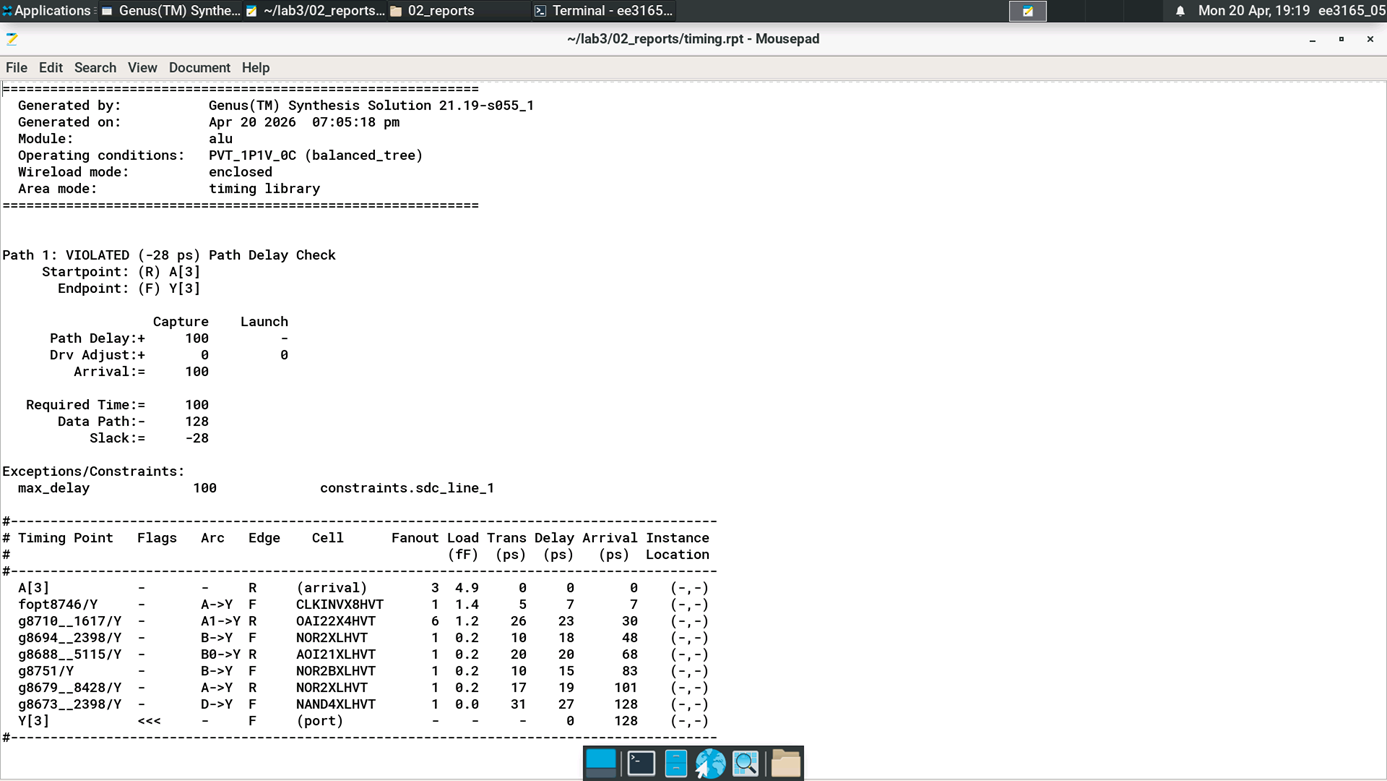
\includegraphics[width=0.8\linewidth]{figure/exp1_path1_report_corner1.png}
    \caption{Chi tiết báo cáo thời gian của đường truyền tới hạn (Path 1) tại góc Fast 1.0V HVT} %[cite: 3]
    \label{fig:exp1_path1_report}
\end{figure}

Đường truyền bắt đầu từ ngõ vào \texttt{A[3]} và kết thúc tại ngõ ra \texttt{Y[3]}. %[cite: 3]
\begin{itemize}
    \item \textbf{Đường đi tín hiệu:} A[3] $\rightarrow$ CLKINVX8HVT $\rightarrow$ OAI22X4HVT $\rightarrow$ NOR2XLHVT $\rightarrow$ AOI21XLHVT $\rightarrow$ NOR2BXLHVT $\rightarrow$ NOR2XLHVT $\rightarrow$ NAND4XLHVT $\rightarrow$ Y[3]. %[cite: 3]
    \item \textbf{Độ trễ đường truyền:} 128 ps.
    \item \textbf{Thời gian yêu cầu:} 100 ps.
    \item \textbf{Thời gian dư (Slack):} 100 ps - 128 ps = -28 ps (Vi phạm). %[cite: 3]
    \item \textbf{Kết luận:} Do thời gian dư mang giá trị âm, đường truyền này đã vi phạm nghiêm trọng yêu cầu về thời gian đặt ra ban đầu. %[cite: 3]
\end{itemize}

\begin{figure}[H]
    \centering
    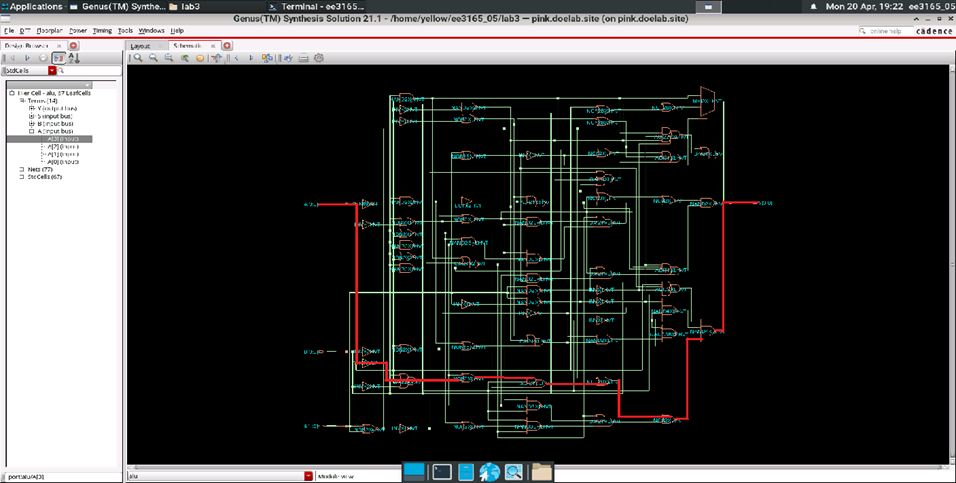
\includegraphics[width=0.8\linewidth]{figure/exp1_path1_schematic_corner1.png}
    \caption{Sơ đồ mạch hiển thị đường truyền tới hạn (Path 1)}
    \label{fig:exp1_path1_schematic}
\end{figure}

\textbf{B. Chi tiết báo cáo các đường truyền vi phạm khác (Từ 2 đến 10)} \\
Bên cạnh đường truyền tới hạn, 9 đường truyền có độ trễ cao tiếp theo cũng đều ghi nhận tình trạng vi phạm thời gian. Dưới đây là kết quả chi tiết trích xuất từ công cụ:

\begin{figure}[H]
    \centering
    \begin{minipage}{0.48\textwidth}
        \centering
        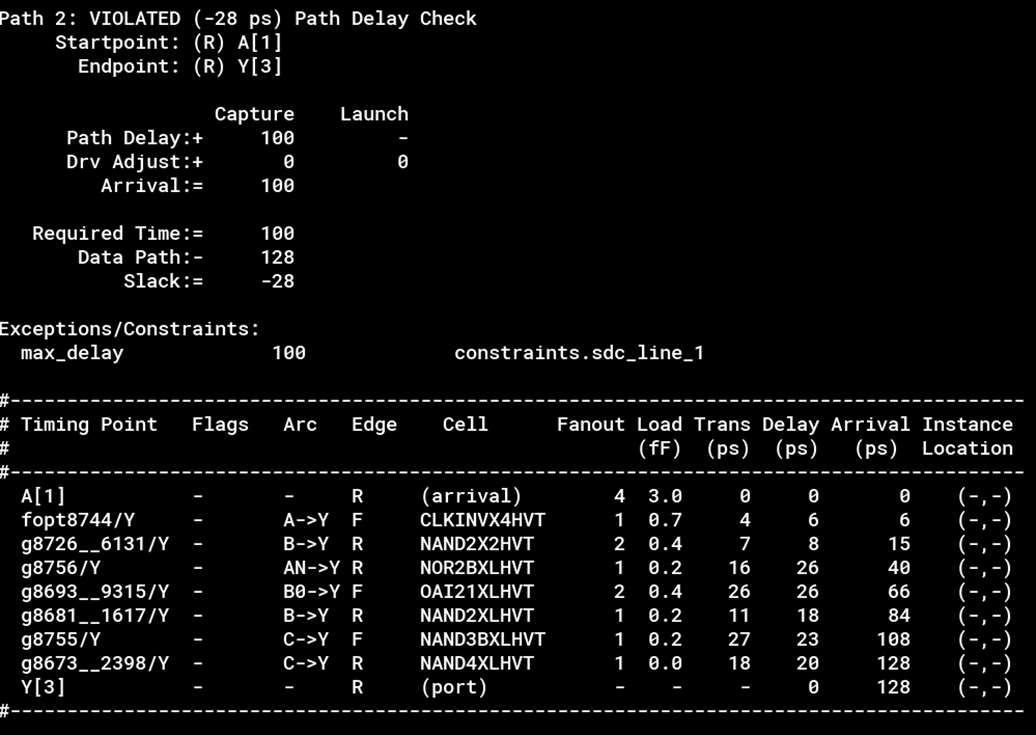
\includegraphics[width=\linewidth]{figure/exp1_path2_report_corner1.png}
        \caption{Báo cáo thời gian Path 2} 
    \end{minipage}\hfill
    \begin{minipage}{0.48\textwidth}
        \centering
        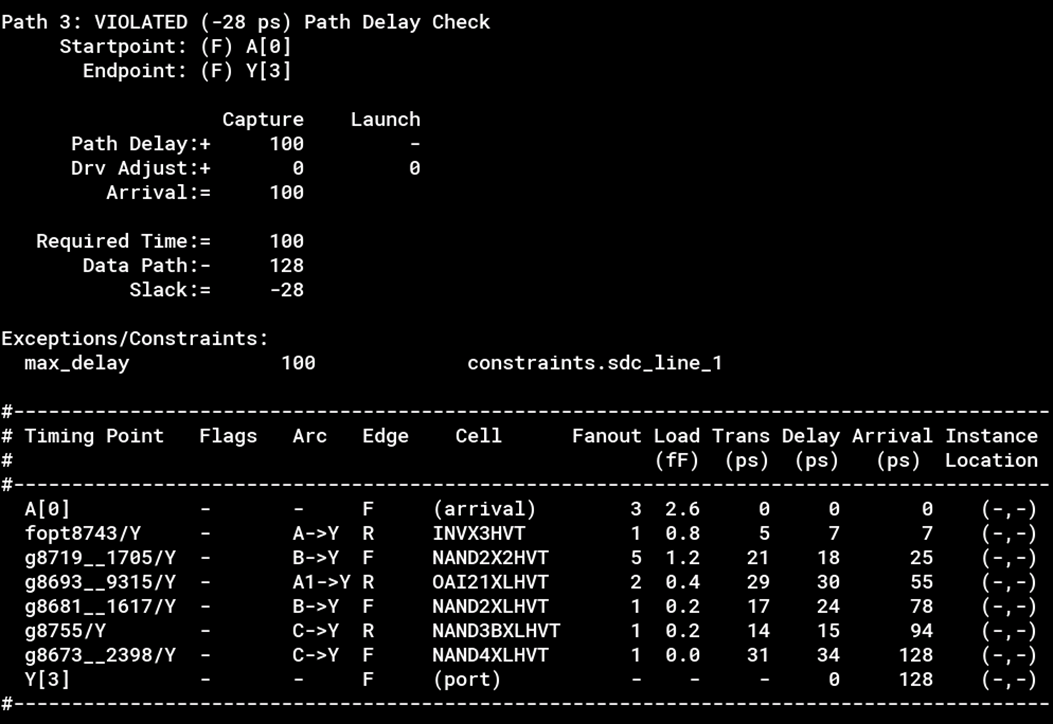
\includegraphics[width=\linewidth]{figure/exp1_path3_report_corner1.png}
        \caption{Báo cáo thời gian Path 3} 
    \end{minipage}
\end{figure}

\begin{figure}[H]
    \centering
    \begin{minipage}{0.48\textwidth}
        \centering
        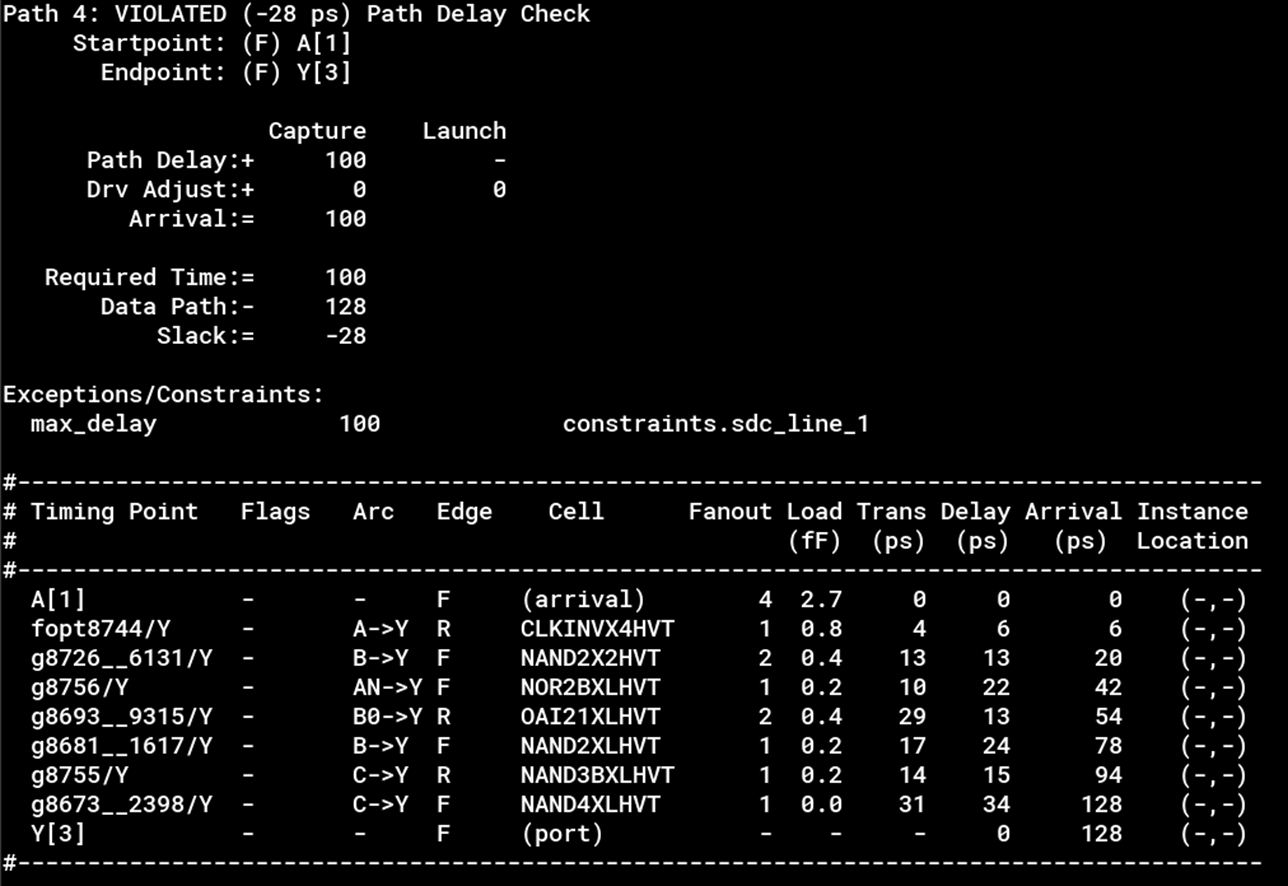
\includegraphics[width=\linewidth]{figure/exp1_path4_report_corner1.png}
        \caption{Báo cáo thời gian Path 4}
    \end{minipage}\hfill
    \begin{minipage}{0.48\textwidth}
        \centering
        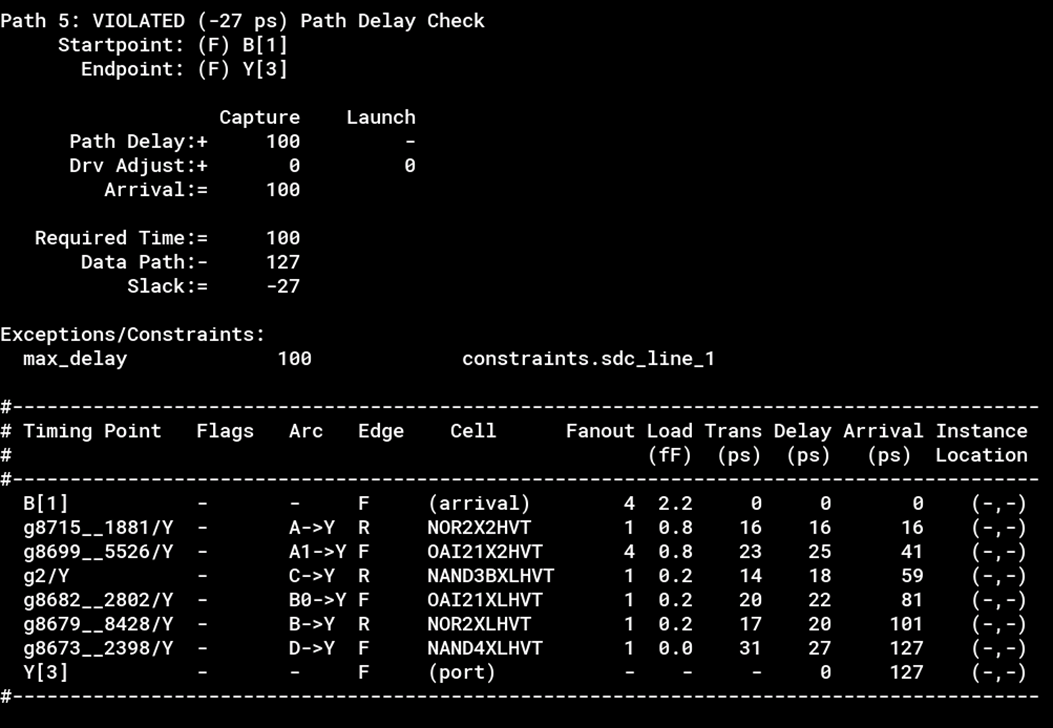
\includegraphics[width=\linewidth]{figure/exp1_path5_report_corner1.png}
        \caption{Báo cáo thời gian Path 5}
    \end{minipage}
\end{figure}

\begin{figure}[H]
    \centering
    \begin{minipage}{0.48\textwidth}
        \centering
        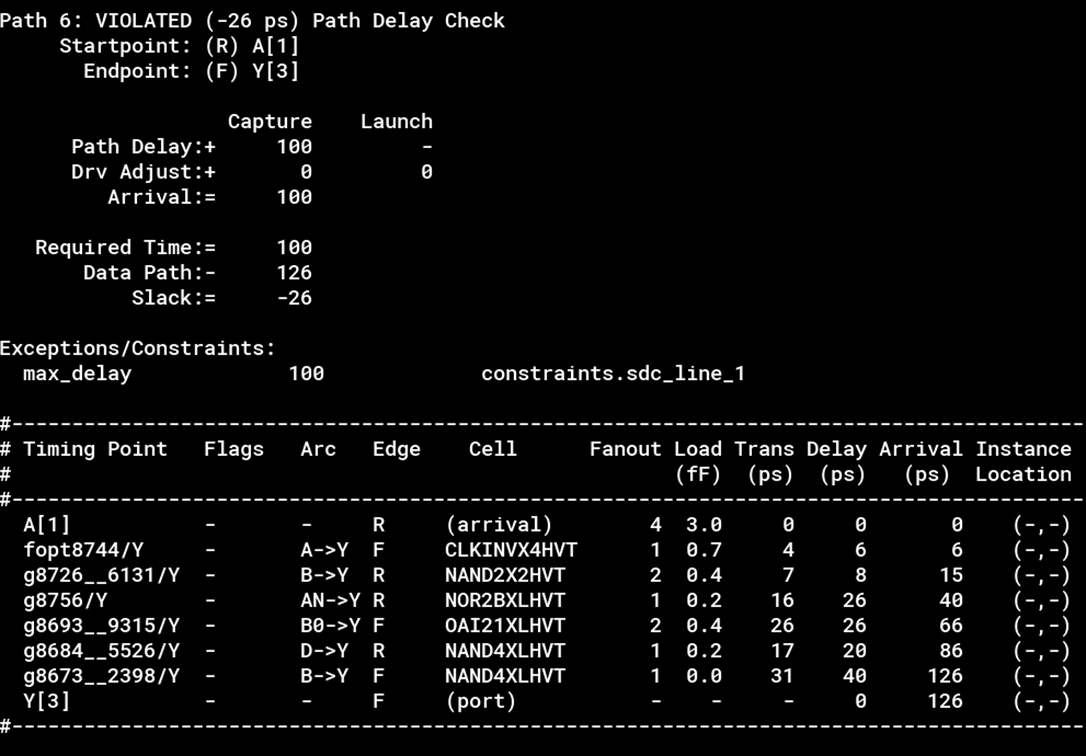
\includegraphics[width=\linewidth]{figure/exp1_path6_report_corner1.png}
        \caption{Báo cáo thời gian Path 6} 
    \end{minipage}\hfill
    \begin{minipage}{0.48\textwidth}
        \centering
        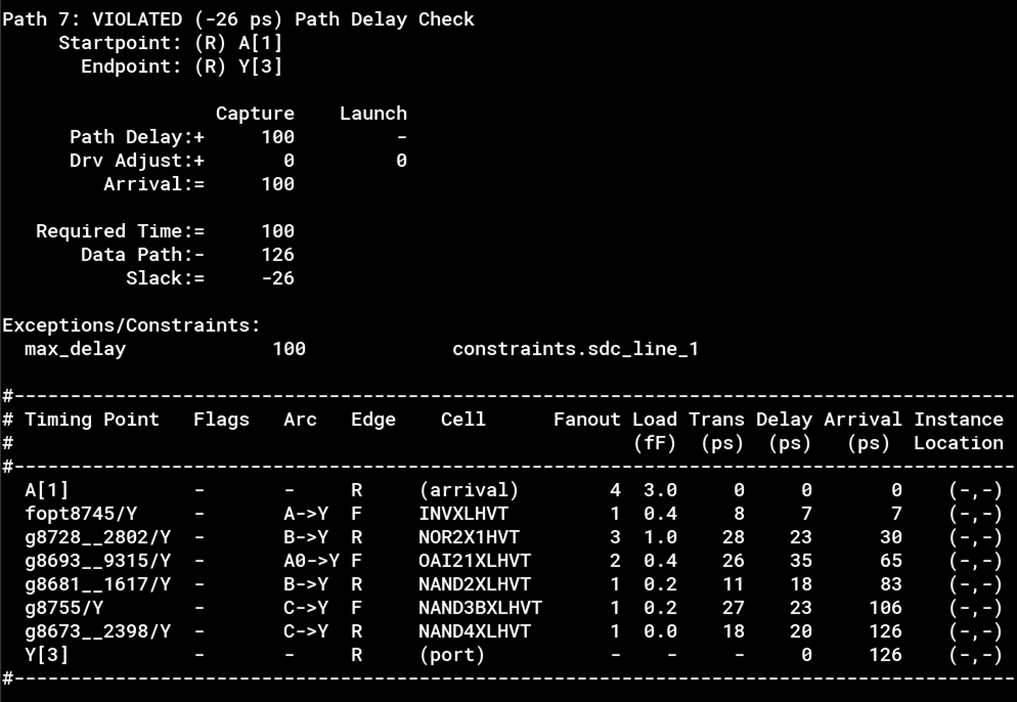
\includegraphics[width=\linewidth]{figure/exp1_path7_report_corner1.png
        }
        \caption{Báo cáo thời gian Path 7} 
    \end{minipage}
\end{figure}

\begin{figure}[H]
    \centering
    \begin{minipage}{0.48\textwidth}
        \centering
        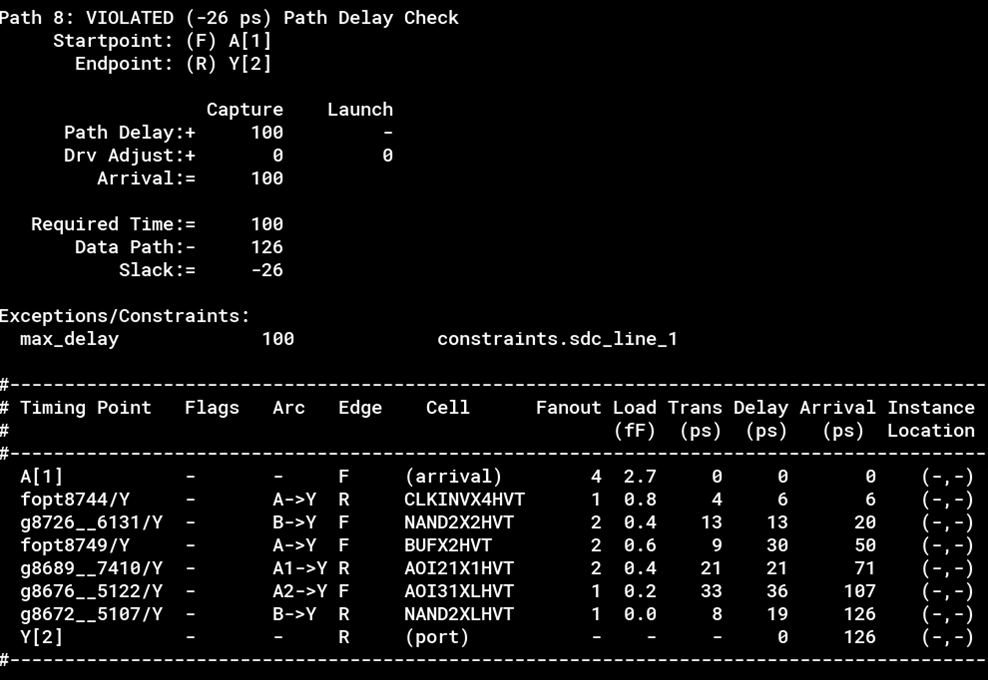
\includegraphics[width=\linewidth]{figure/exp1_path8_report_corner1.png}
        \caption{Báo cáo thời gian Path 8} 
    \end{minipage}\hfill
    \begin{minipage}{0.48\textwidth}
        \centering
        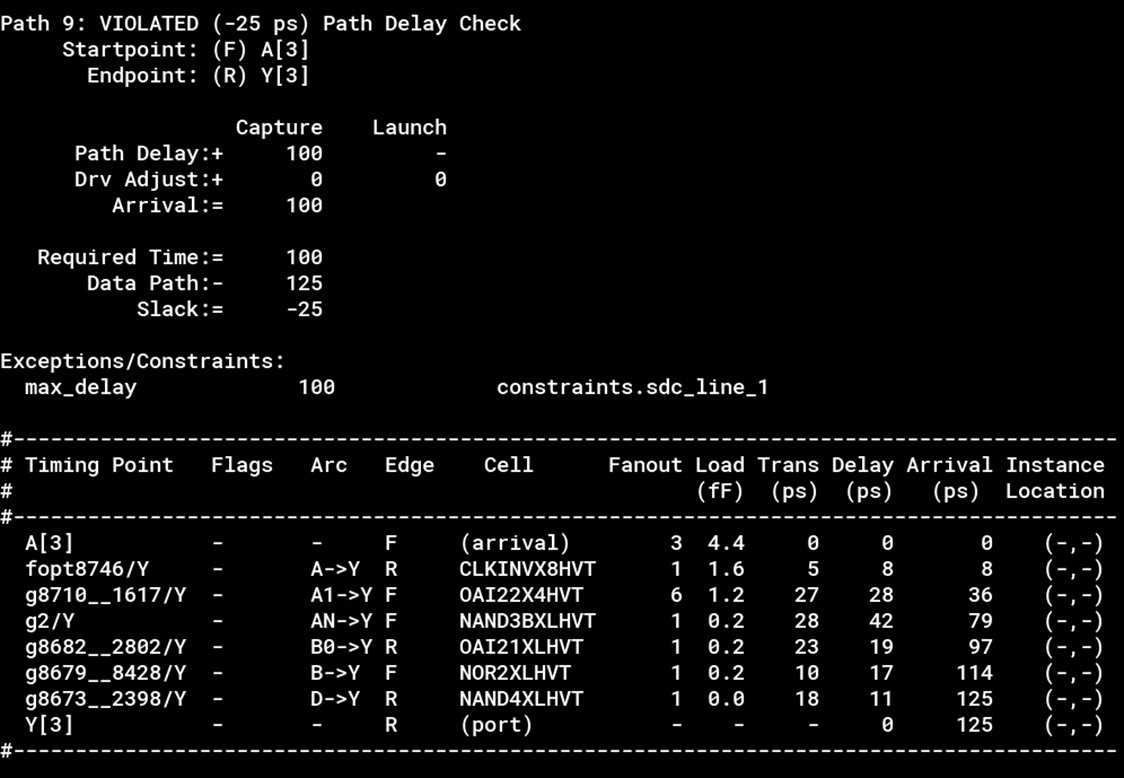
\includegraphics[width=\linewidth]{figure/exp1_path9_report_corner1.png}
        \caption{Báo cáo thời gian Path 9} 
    \end{minipage}
\end{figure}

\begin{figure}[H]
    \centering
    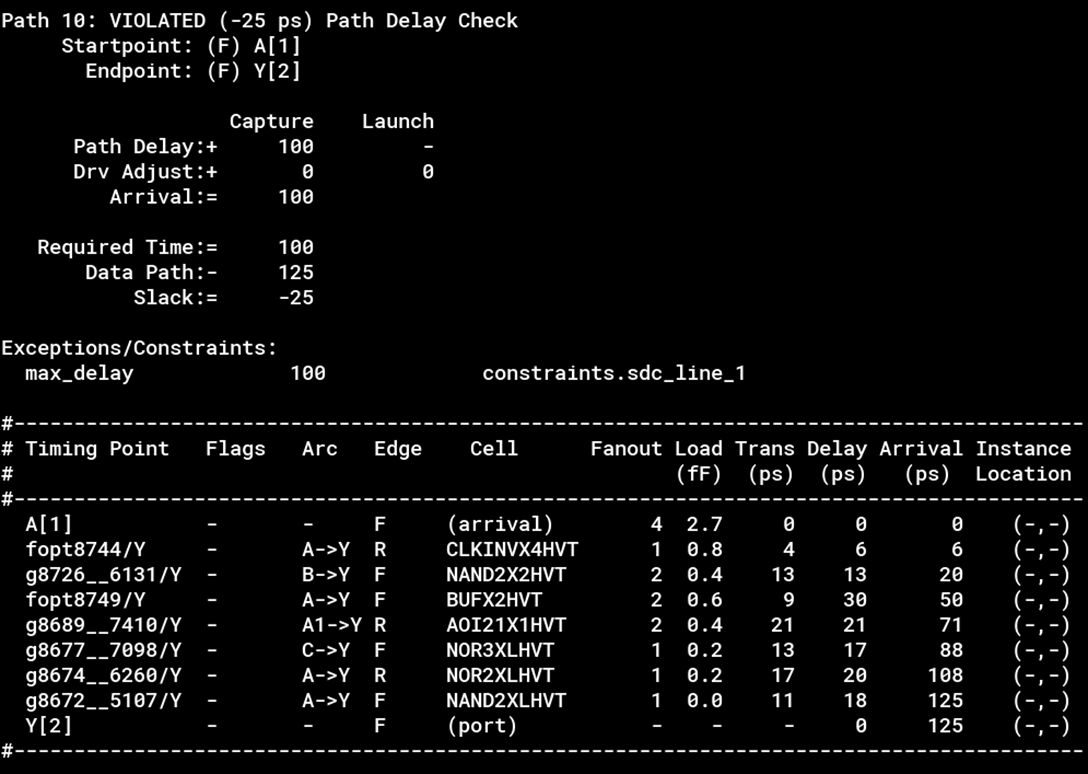
\includegraphics[width=0.48\linewidth]{figure/exp1_path10_report_corner1.png}
    \caption{Báo cáo thời gian Path 10} 
    \label{fig:exp1_path10}
\end{figure}

\textbf{C. Bảng tổng hợp 10 đường truyền trễ nhất}
\begin{table}[H]
    \centering
    \resizebox{\textwidth}{!}{
    \begin{tabular}{|c|p{12.5cm}|c|c|}
        \hline
        \textbf{STT} & \textbf{Đường đi tín hiệu} & \textbf{Độ trễ (ps)} & \textbf{Thời gian dư (ps)} \\
        \hline
        1 & A[3] $\rightarrow$ CLKINVX8HVT $\rightarrow$ OAI22X4HVT $\rightarrow$ NOR2XLHVT $\rightarrow$ AOI21XLHVT $\rightarrow$ NOR2BXLHVT $\rightarrow$ NOR2XLHVT $\rightarrow$ NAND4XLHVT $\rightarrow$ Y[3] & 128 & -28 (Vi phạm) \\ \hline %[cite: 3]
        2 & A[1] $\rightarrow$ CLKINVX4HVT $\rightarrow$ NAND2X2HVT $\rightarrow$ NOR2BXLHVT $\rightarrow$ OAI21XLHVT $\rightarrow$ NAND2XLHVT $\rightarrow$ NAND3BXLHVT $\rightarrow$ NAND4XLHVT $\rightarrow$ Y[3] & 128 & -28 (Vi phạm) \\ \hline %[cite: 3]
        3 & A[0] $\rightarrow$ INVX3HVT $\rightarrow$ NAND2X2HVT $\rightarrow$ OAI21XLHVT $\rightarrow$ NAND2XLHVT $\rightarrow$ NAND3BXLHVT $\rightarrow$ NAND4XLHVT $\rightarrow$ Y[3] & 128 & -28 (Vi phạm) \\ \hline %[cite: 3]
        4 & A[1] $\rightarrow$ CLKINVX4HVT $\rightarrow$ NAND2X2HVT $\rightarrow$ NOR2BXLHVT $\rightarrow$ OAI21XLHVT $\rightarrow$ NAND2XLHVT $\rightarrow$ NAND3BXLHVT $\rightarrow$ NAND4XLHVT $\rightarrow$ Y[3] & 128 & -28 (Vi phạm) \\ \hline %[cite: 3]
        5 & B[1] $\rightarrow$ NOR2X2HVT $\rightarrow$ OAI21X2HVT $\rightarrow$ NAND3BXLHVT $\rightarrow$ OAI21XLHVT $\rightarrow$ NOR2XLHVT $\rightarrow$ NAND4XLHVT $\rightarrow$ Y[3] & 127 & -27 (Vi phạm) \\ \hline %[cite: 3]
        6 & A[1] $\rightarrow$ CLKINVX4HVT $\rightarrow$ NAND2X2HVT $\rightarrow$ NOR2BXLHVT $\rightarrow$ OAI21XLHVT $\rightarrow$ NAND4XLHVT $\rightarrow$ Y[3] & 126 & -26 (Vi phạm) \\ \hline %[cite: 3]
        7 & A[1] $\rightarrow$ INVXLHVT $\rightarrow$ NOR2X1HVT $\rightarrow$ OAI21XLHVT $\rightarrow$ NAND2XLHVT $\rightarrow$ NAND3BXLHVT $\rightarrow$ NAND4XLHVT $\rightarrow$ Y[3] & 126 & -26 (Vi phạm) \\ \hline %[cite: 3]
        8 & A[1] $\rightarrow$ CLKINVX4HVT $\rightarrow$ NAND2X2HVT $\rightarrow$ BUFX2HVT $\rightarrow$ AOI21X1HVT $\rightarrow$ AOI31XLHVT $\rightarrow$ NAND2XLHVT $\rightarrow$ Y[2] & 126 & -26 (Vi phạm) \\ \hline %[cite: 3]
        9 & A[3] $\rightarrow$ CLKINVX8HVT $\rightarrow$ AOI22X4HVT $\rightarrow$ NAND3BXLHVT $\rightarrow$ OAI21XLHVT $\rightarrow$ NOR2XLHVT $\rightarrow$ NAND4XLHVT $\rightarrow$ Y[3] & 125 & -25 (Vi phạm) \\ \hline %[cite: 3]
        10 & A[1] $\rightarrow$ CLKINVX4HVT $\rightarrow$ NAND2X2HVT $\rightarrow$ BUFX2HVT $\rightarrow$ AOI21X1HVT $\rightarrow$ NOR3XLHVT $\rightarrow$ NOR2XLHVT $\rightarrow$ NAND2XLHVT $\rightarrow$ Y[2] & 125 & -25 (Vi phạm) \\ \hline %[cite: 3]
    \end{tabular}
    }
    \caption{Tổng hợp 10 đường truyền trễ nhất - Góc Nhanh 1.0V HVT}
\end{table}

\textbf{D. Nhận xét phân tích} \\
Kết quả mô phỏng cho thấy ở góc vận hành Nhanh (Fast) kết hợp với mức điện áp thấp 1.0V, toàn bộ 10 đường truyền tới hạn đều vi phạm thời gian (Slack dao động từ -28 ps đến -25 ps). Nguyên nhân cốt lõi là do thư viện \texttt{basicCells\_hvt} bao gồm các phần tử logic có điện áp ngưỡng cao (High-Vt). Khi hạ nguồn cung cấp xuống 1.0V, hiện tượng "đói dòng" xảy ra làm giảm mạnh tốc độ chuyển mạch nạp xả, khiến độ trễ của đường truyền dài nhất (128 ps) vượt quá giới hạn 100 ps một khoảng đáng kể. Ràng buộc thời gian 100 ps (tương đương tần số 10GHz) tỏ ra quá khắt khe đối với cấu hình thư viện và mức điện áp này. %[cite: 3]

% ================= CORNER 2 =================
\subsubsection{Corner 2: Nhanh (FF) - 1.2V - HVT (\texttt{fast\_vdd1v2\_basicCells\_hvt.lib})}

\textbf{A. Phân tích đường truyền tới hạn (Đường truyền số 1)} \\
Dựa trên kết quả tổng hợp và phân tích STA ở điều kiện điện áp 1.2V, đường truyền có độ trễ lớn nhất được xác định với các thông số như sau: %[cite: 3]

\begin{figure}[H]
    \centering
    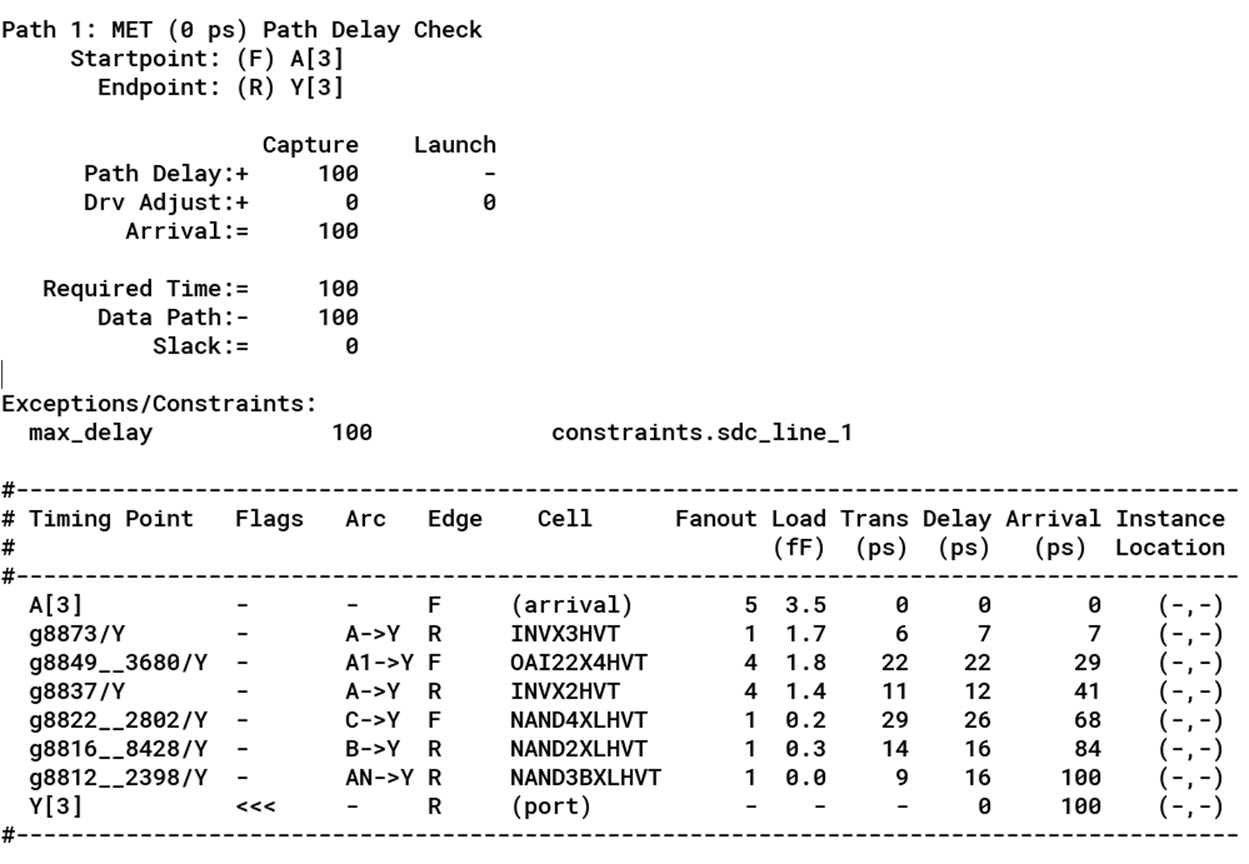
\includegraphics[width=0.8\linewidth]{figure/exp1_path1_report_corner2.png}
    \caption{Chi tiết báo cáo thời gian của đường truyền tới hạn (Path 1) tại góc Fast 1.2V HVT} %[cite: 3]
    \label{fig:exp1_c2_path1_report}
\end{figure}

Đường truyền bắt đầu từ ngõ vào \texttt{A[3]} và kết thúc tại ngõ ra \texttt{Y[3]}. %[cite: 3]
\begin{itemize}
    \item \textbf{Đường đi tín hiệu:} A[3] $\rightarrow$ INVX3HVT $\rightarrow$ OAI22X4HVT $\rightarrow$ INVX2HVT $\rightarrow$ NAND4XLHVT $\rightarrow$ NAND2XLHVT $\rightarrow$ NAND3BXLHVT $\rightarrow$ Y[3]. %[cite: 3]
    \item \textbf{Độ trễ đường truyền:} 100 ps. %[cite: 3]
    \item \textbf{Thời gian yêu cầu:} 100 ps. %[cite: 3]
    \item \textbf{Thời gian dư (Slack):} 100 ps - 100 ps = 0 ps (Đạt). %[cite: 3]
    \item \textbf{Kết luận:} Với Slack $\ge$ 0, đường truyền này đáp ứng vừa đủ (marginal met) yêu cầu về thời gian đã đặt ra, không có sự vi phạm timing. %[cite: 3]
\end{itemize}

\begin{figure}[H]
    \centering
    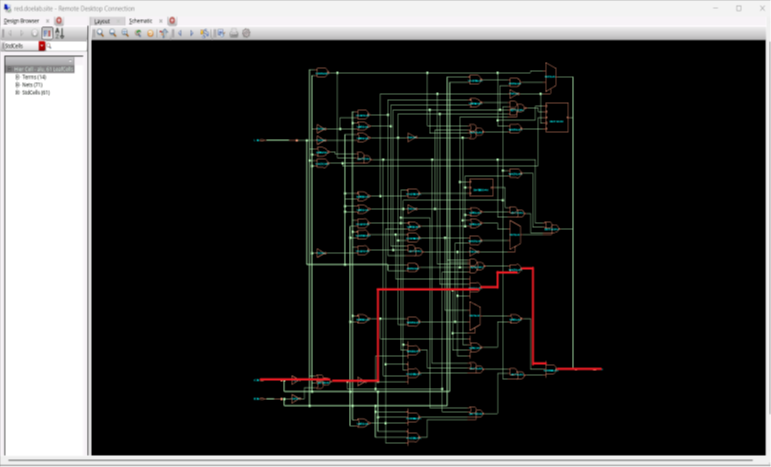
\includegraphics[width=0.8\linewidth]{figure/exp1_path1_schematic_corner2.png}
    \caption{Sơ đồ mạch hiển thị đường truyền tới hạn (Path 1) tại góc Fast 1.2V HVT} %[cite: 3]
    \label{fig:exp1_c2_path1_schematic}
\end{figure}

\textbf{B. Chi tiết báo cáo các đường truyền khác (Từ 2 đến 10)} \\
Tương tự như đường truyền tới hạn, 9 đường truyền có độ trễ cao tiếp theo đều đạt trạng thái an toàn (MET). Dưới đây là kết quả chi tiết trích xuất từ công cụ: %[cite: 3]

\begin{figure}[H]
    \centering
    \begin{minipage}{0.48\textwidth}
        \centering
        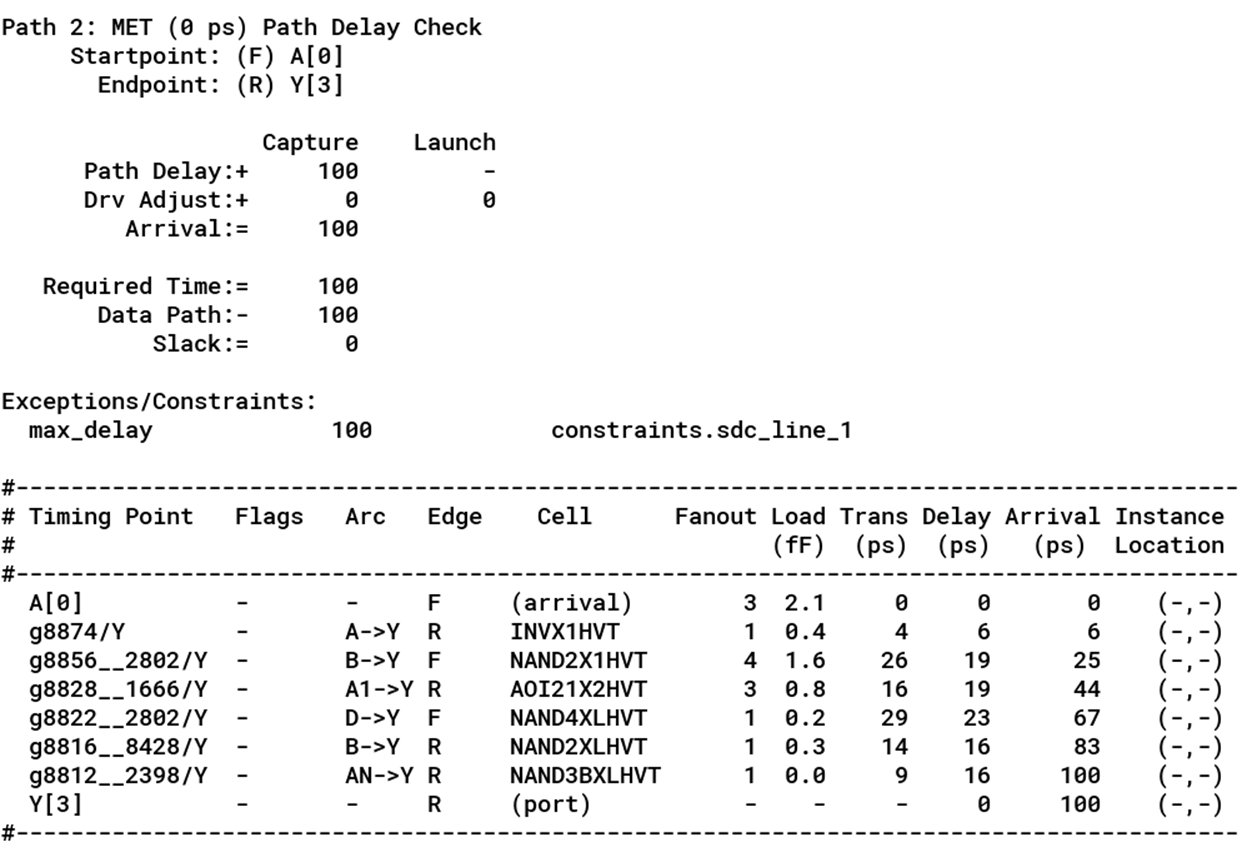
\includegraphics[width=\linewidth]{figure/exp1_path2_report_corner2.png}
        \caption{Báo cáo thời gian Path 2} %[cite: 3]
    \end{minipage}\hfill
    \begin{minipage}{0.48\textwidth}
        \centering
        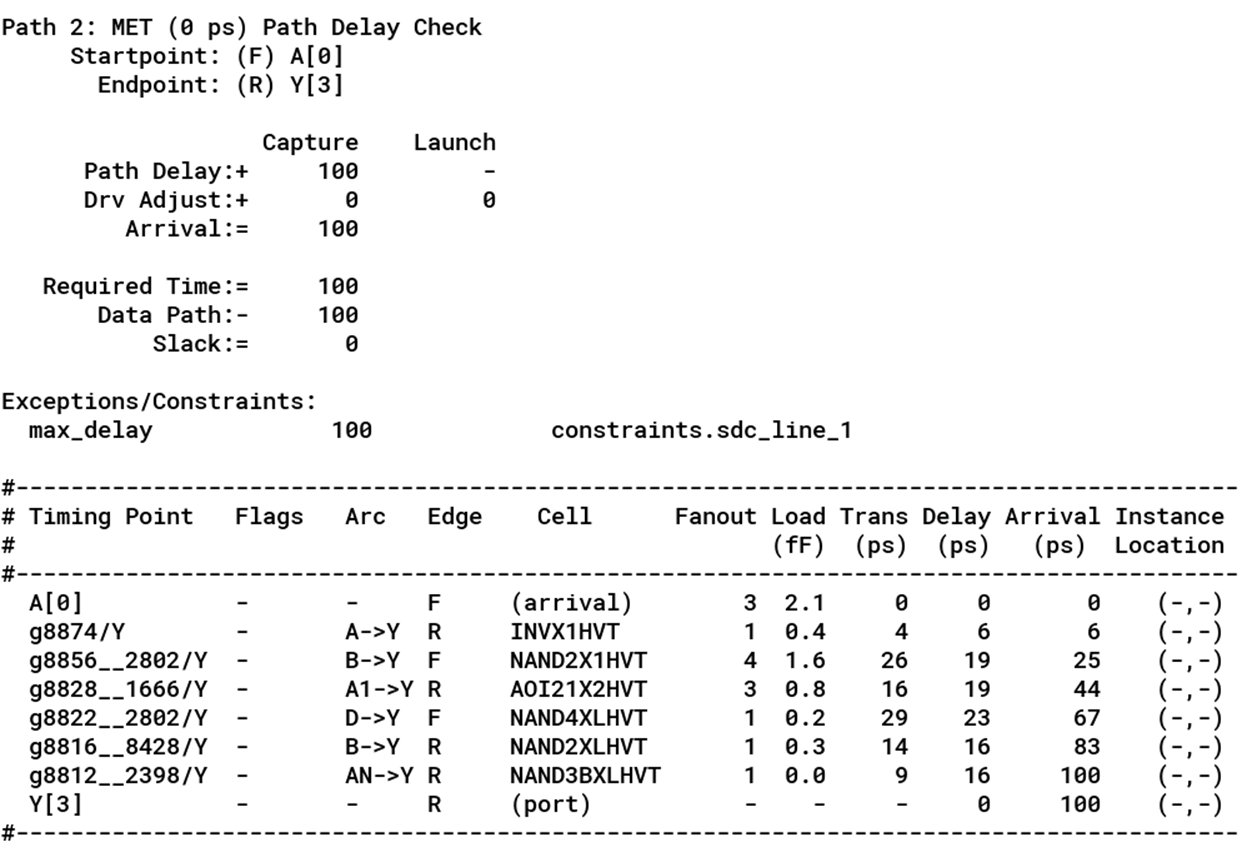
\includegraphics[width=\linewidth]{figure/exp1_path2_report_corner2.png}
        \caption{Báo cáo thời gian Path 3} %[cite: 3]
    \end{minipage}
\end{figure}

\begin{figure}[H]
    \centering
    \begin{minipage}{0.48\textwidth}
        \centering
        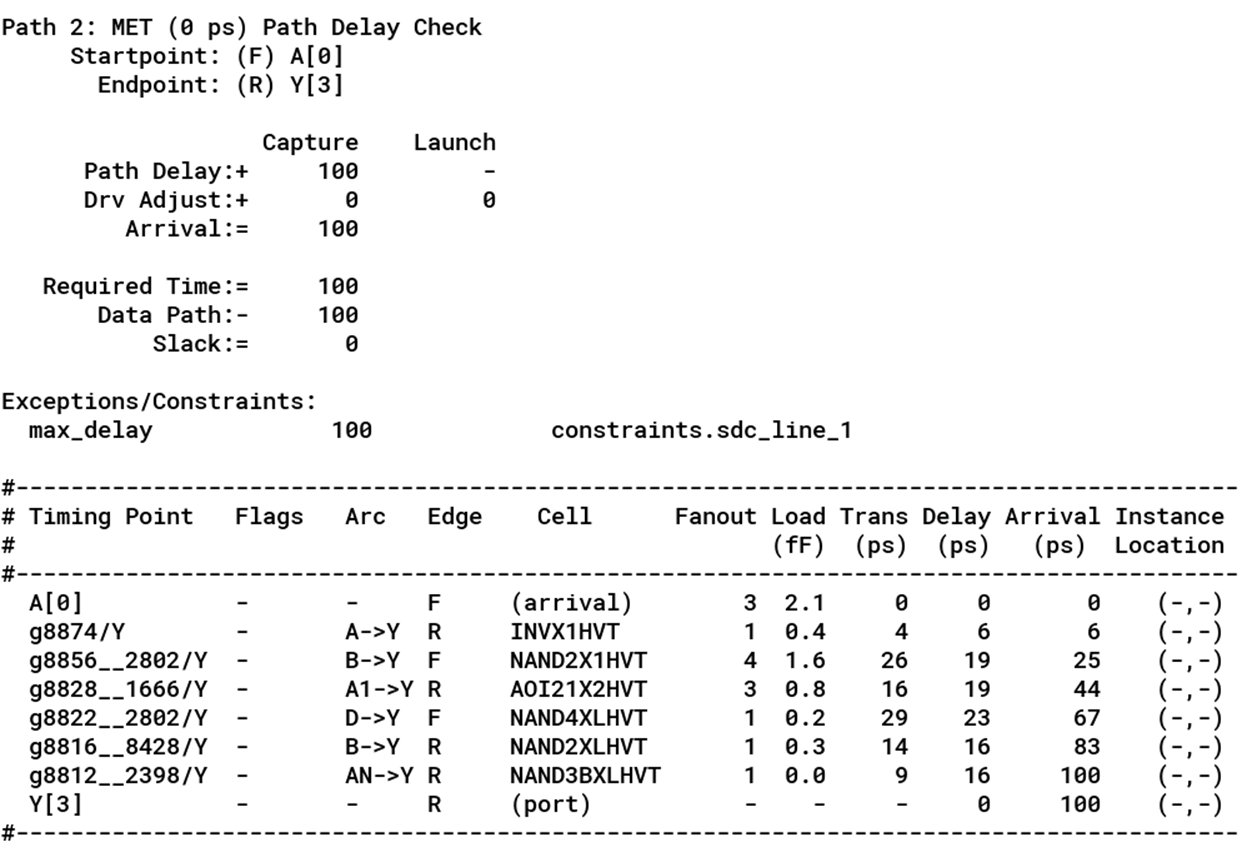
\includegraphics[width=\linewidth]{figure/exp1_path2_report_corner2.png}
        \caption{Báo cáo thời gian Path 4} %[cite: 3]
    \end{minipage}\hfill
    \begin{minipage}{0.48\textwidth}
        \centering
        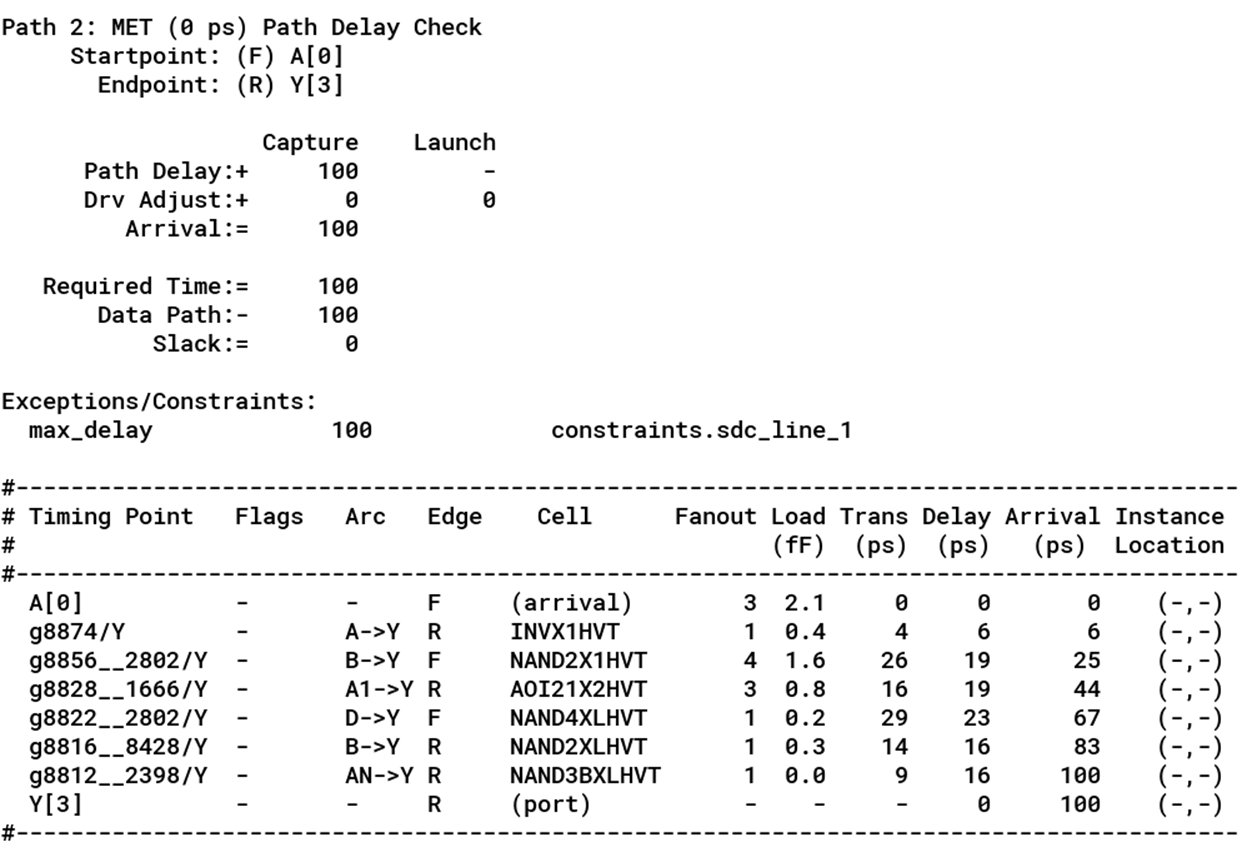
\includegraphics[width=\linewidth]{figure/exp1_path2_report_corner2.png}
        \caption{Báo cáo thời gian Path 5} %[cite: 3]
    \end{minipage}
\end{figure}

\begin{figure}[H]
    \centering
    \begin{minipage}{0.48\textwidth}
        \centering
        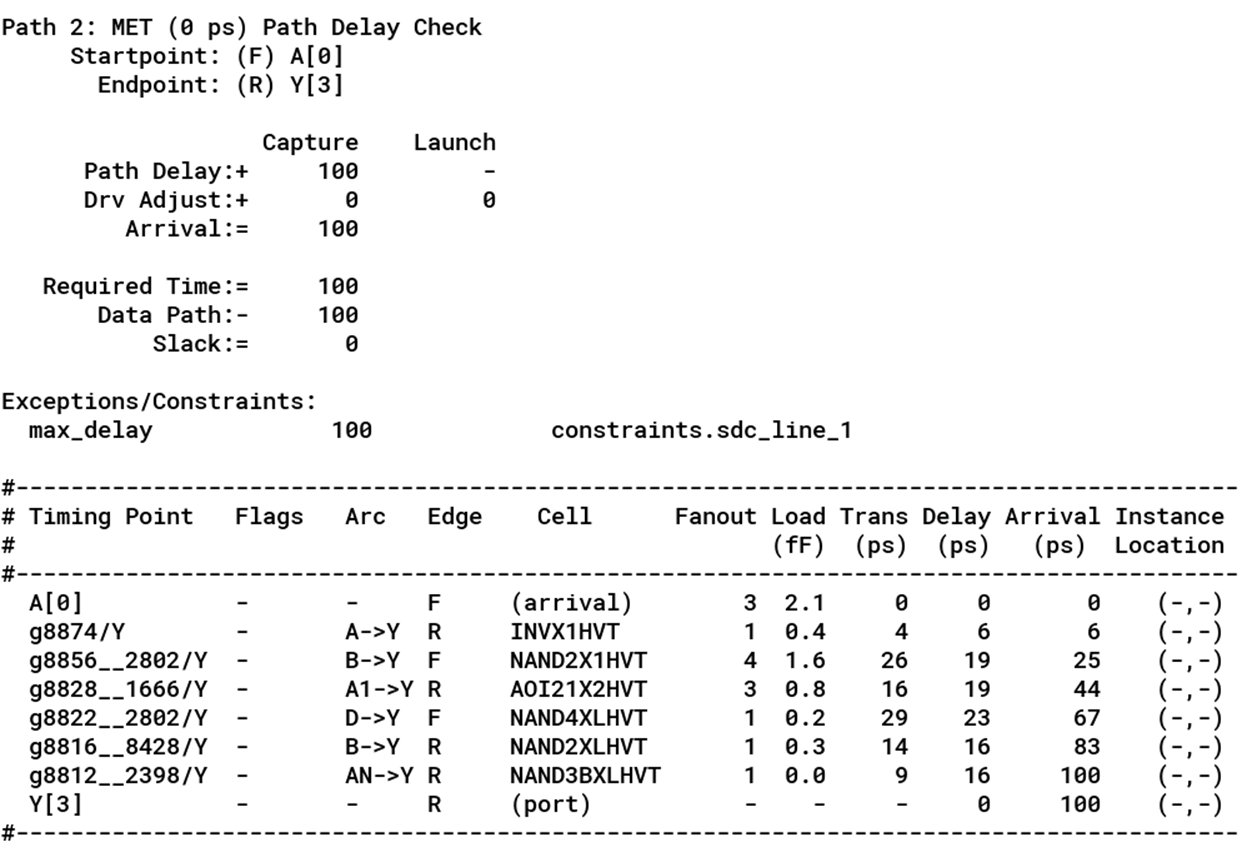
\includegraphics[width=\linewidth]{figure/exp1_path2_report_corner2.png}
        \caption{Báo cáo thời gian Path 6} %[cite: 3]
    \end{minipage}\hfill
    \begin{minipage}{0.48\textwidth}
        \centering
        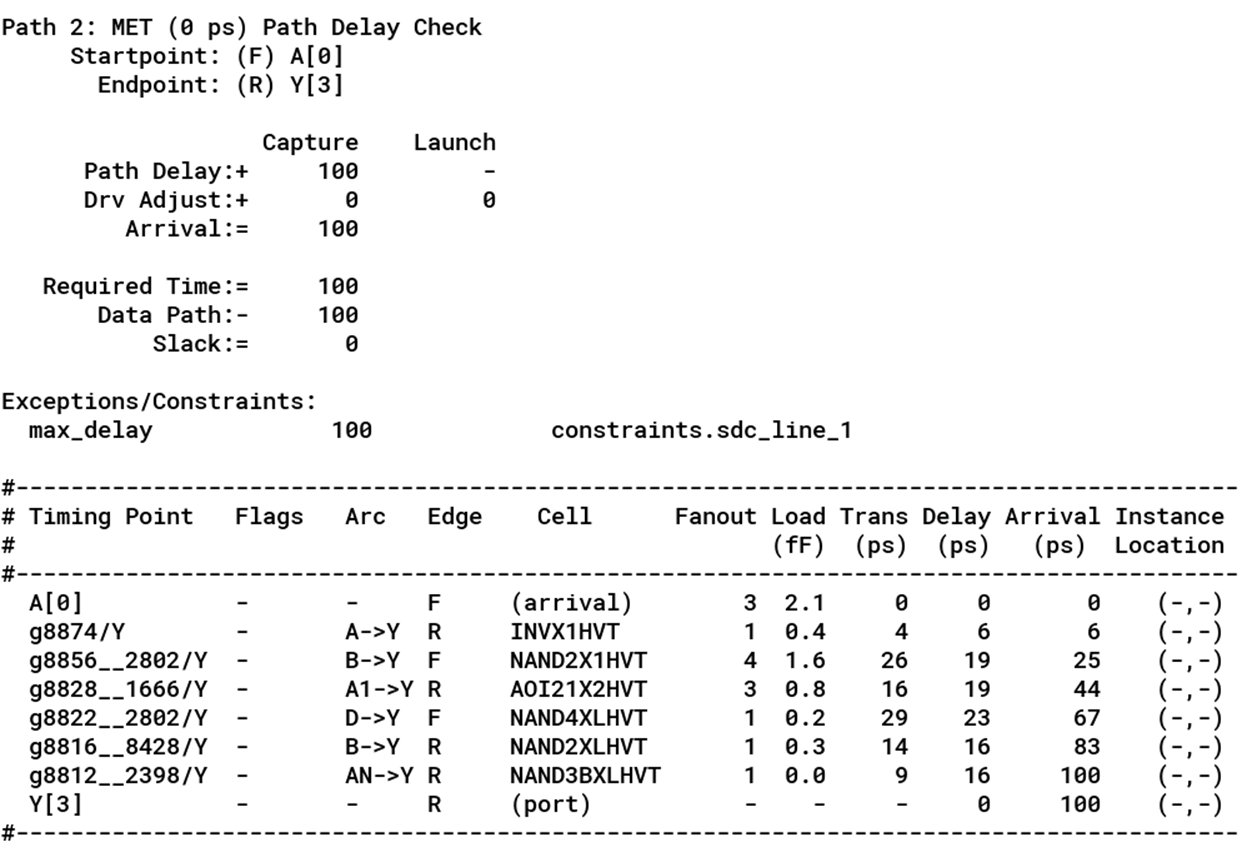
\includegraphics[width=\linewidth]{figure/exp1_path2_report_corner2.png}
        \caption{Báo cáo thời gian Path 7} %[cite: 3]
    \end{minipage}
\end{figure}

\begin{figure}[H]
    \centering
    \begin{minipage}{0.48\textwidth}
        \centering
        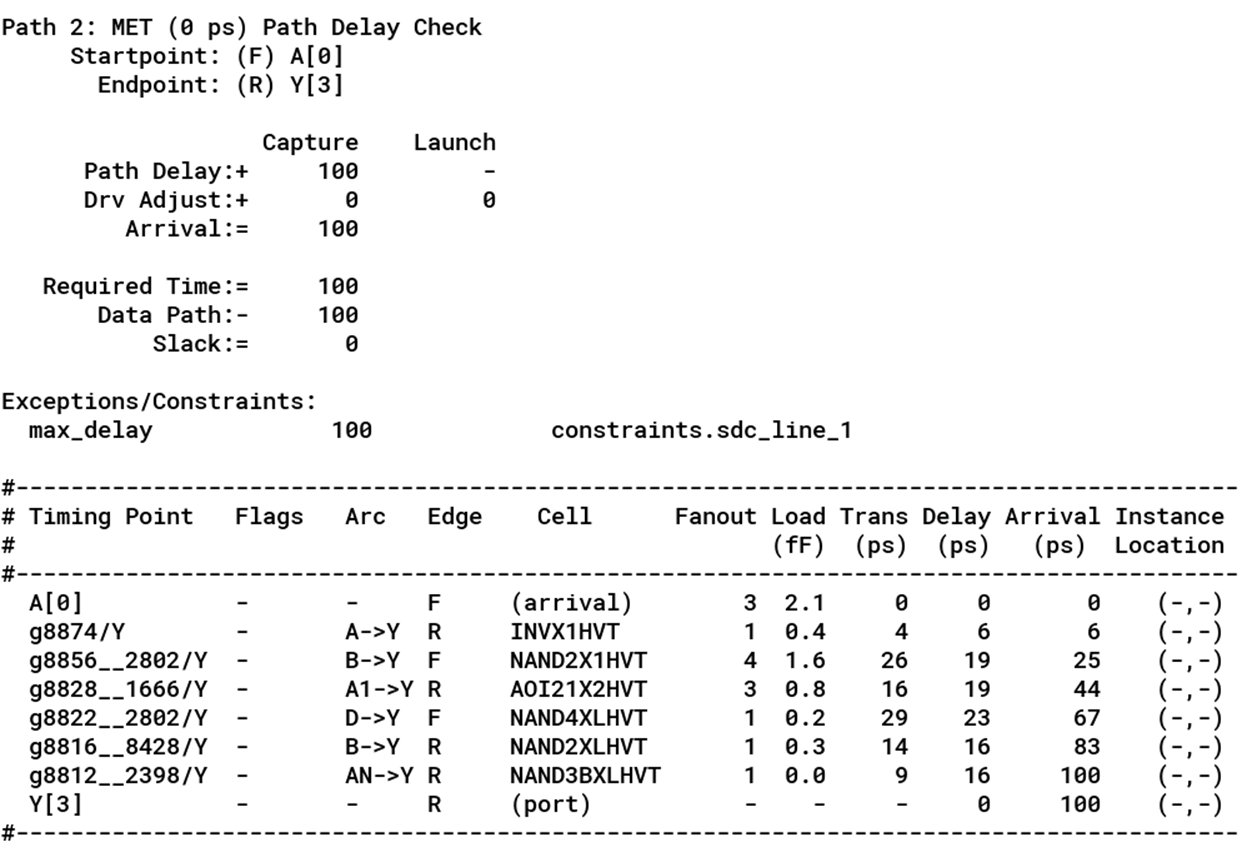
\includegraphics[width=\linewidth]{figure/exp1_path2_report_corner2.png}
        \caption{Báo cáo thời gian Path 8} %[cite: 3]
    \end{minipage}\hfill
    \begin{minipage}{0.48\textwidth}
        \centering
        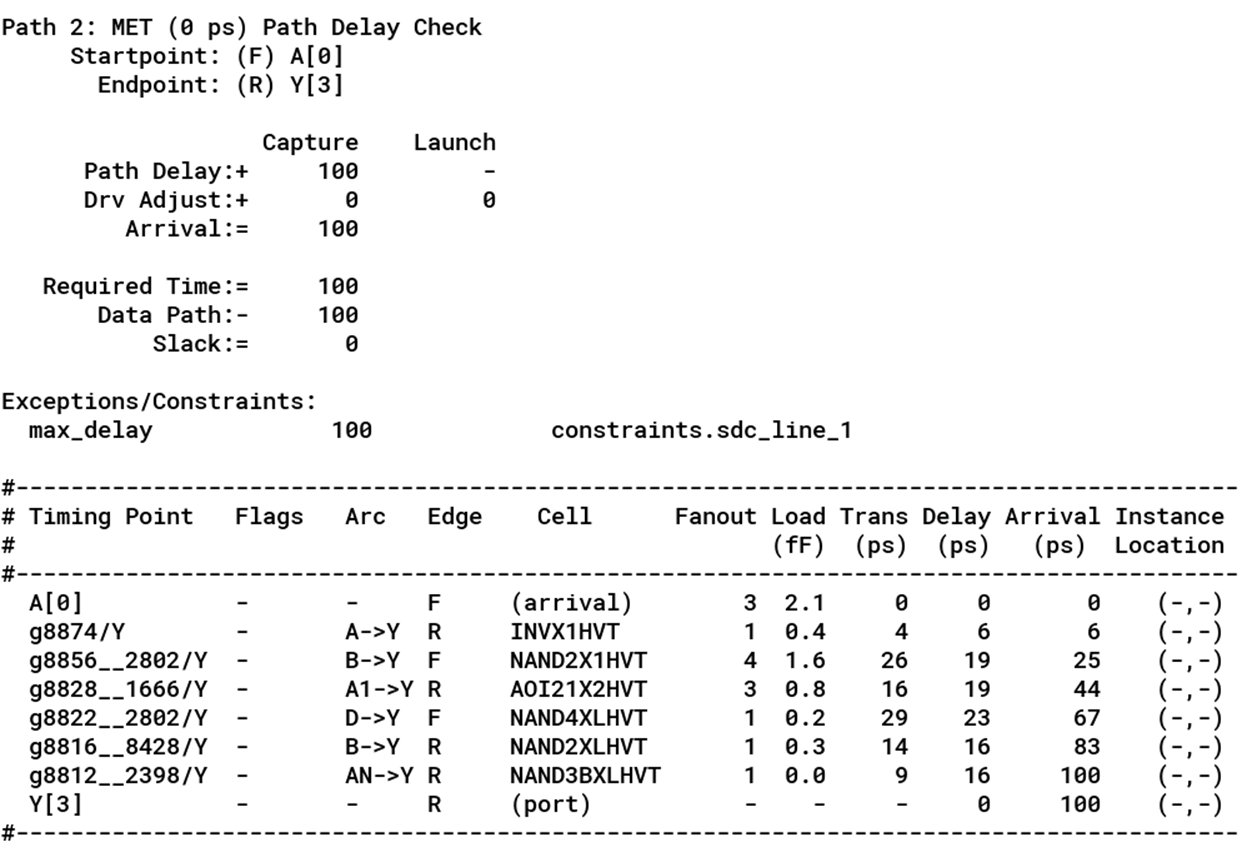
\includegraphics[width=\linewidth]{figure/exp1_path2_report_corner2.png}
        \caption{Báo cáo thời gian Path 9} %[cite: 3]
    \end{minipage}
\end{figure}

\begin{figure}[H]
    \centering
    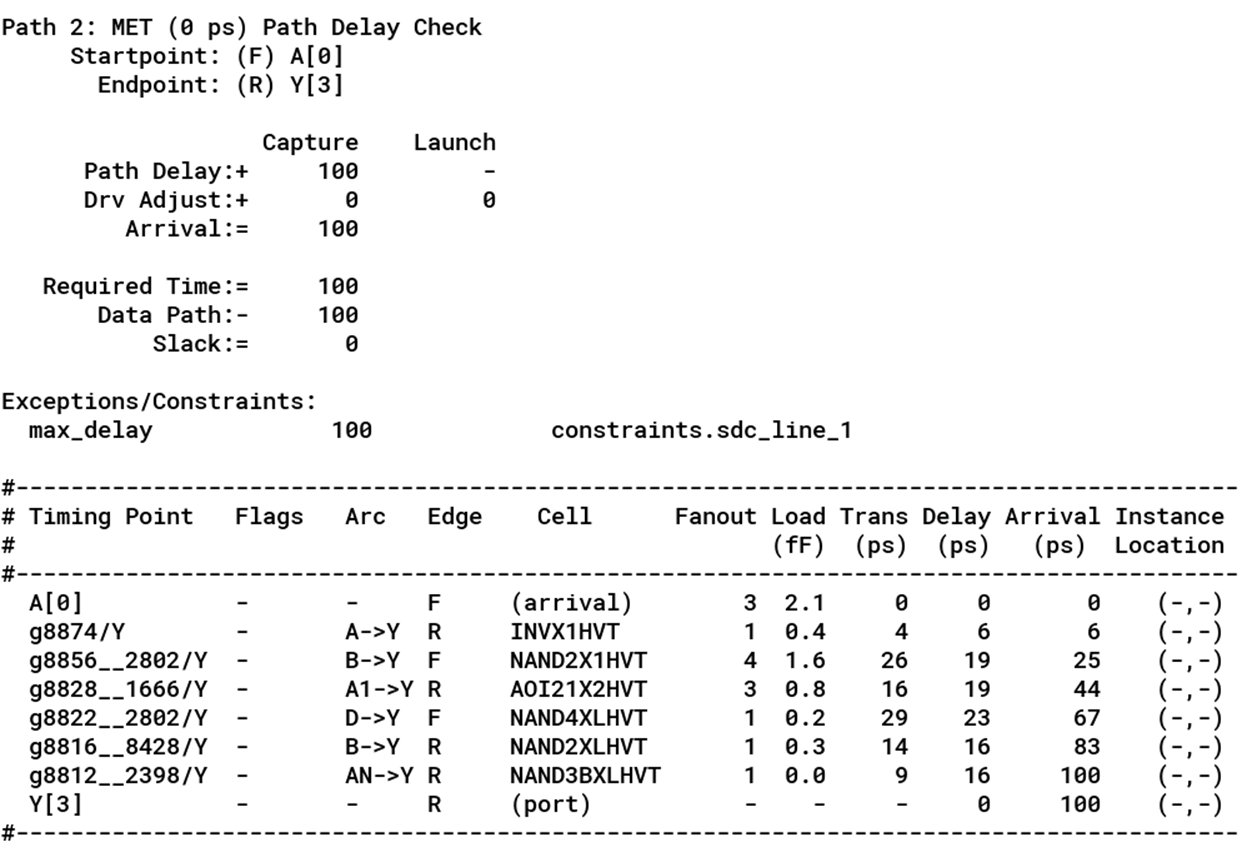
\includegraphics[width=0.48\linewidth]{figure/exp1_path2_report_corner2.png}
    \caption{Báo cáo thời gian Path 10} %[cite: 3]
    \label{fig:exp1_c2_path10}
\end{figure}

\textbf{C. Bảng tổng hợp 10 đường truyền trễ nhất}
\begin{table}[H]
    \centering
    \resizebox{\textwidth}{!}{
    \begin{tabular}{|c|p{12.5cm}|c|c|}
        \hline
        \textbf{STT} & \textbf{Đường đi tín hiệu} & \textbf{Độ trễ (ps)} & \textbf{Thời gian dư (ps)} \\
        \hline
        1 & A[3] $\rightarrow$ INVX3HVT $\rightarrow$ OAI22X4HVT $\rightarrow$ INVX2HVT $\rightarrow$ NAND4XLHVT $\rightarrow$ NAND2XLHVT $\rightarrow$ NAND3BXLHVT $\rightarrow$ Y[3] & 100 & 0 (Đạt) \\ \hline %[cite: 3]
        2 & A[0] $\rightarrow$ INVX1HVT $\rightarrow$ NAND2X1HVT $\rightarrow$ AOI21X2HVT $\rightarrow$ NAND4XLHVT $\rightarrow$ NAND2XLHVT $\rightarrow$ NAND3BXLHVT $\rightarrow$ Y[3] & 100 & 0 (Đạt) \\ \hline %[cite: 3]
        3 & A[1] $\rightarrow$ INVX1HVT $\rightarrow$ NAND2X1HVT $\rightarrow$ AOI21X2HVT $\rightarrow$ NAND4XLHVT $\rightarrow$ NAND2XLHVT $\rightarrow$ NAND3BXLHVT $\rightarrow$ Y[3] & 99 & +1 (Đạt) \\ \hline %[cite: 3]
        4 & B[0] $\rightarrow$ NAND2X4HVT $\rightarrow$ OAI21X2HVT $\rightarrow$ NAND4BXLHVT $\rightarrow$ OAI21XLHVT $\rightarrow$ AOI21XLHVT $\rightarrow$ NAND3BXLHVT $\rightarrow$ Y[3] & 99 & +1 (Đạt) \\ \hline %[cite: 3]
        5 & A[3] $\rightarrow$ INVX3HVT $\rightarrow$ OAI22X4HVT $\rightarrow$ INVX2HVT $\rightarrow$ NAND4BXLHVT $\rightarrow$ OAI21XLHVT $\rightarrow$ AOI21XLHVT $\rightarrow$ NAND3BXLHVT $\rightarrow$ Y[3] & 99 & +1 (Đạt) \\ \hline %[cite: 3]
        6 & B[2] $\rightarrow$ NAND2X2HVT $\rightarrow$ NOR2BX1HVT $\rightarrow$ OAI2BBX1HVT $\rightarrow$ AOI21X1HVT $\rightarrow$ OAI21X1HVT $\rightarrow$ Y[2] & 98 & +2 (Đạt) \\ \hline %[cite: 3]
        7 & S[0] $\rightarrow$ INVX1HVT $\rightarrow$ NOR2X1HVT $\rightarrow$ INVX1HVT $\rightarrow$ NOR4X1HVT $\rightarrow$ NOR2XLHVT $\rightarrow$ NAND3BXLHVT $\rightarrow$ Y[3] & 98 & +2 (Đạt) \\ \hline %[cite: 3]
        8 & B[3] $\rightarrow$ INVX2HVT $\rightarrow$ OAI22X4HVT $\rightarrow$ INVX2HVT $\rightarrow$ NAND4XLHVT $\rightarrow$ NAND2XLHVT $\rightarrow$ NAND3BXLHVT $\rightarrow$ Y[3] & 97 & +3 (Đạt) \\ \hline %[cite: 3]
        9 & B[1] $\rightarrow$ NAND2X1HVT $\rightarrow$ OAI21X2HVT $\rightarrow$ NAND4BXLHVT $\rightarrow$ OAI21XLHVT $\rightarrow$ AOI21XLHVT $\rightarrow$ NAND3BXLHVT $\rightarrow$ Y[3] & 97 & +3 (Đạt) \\ \hline %[cite: 3]
        10 & A[0] $\rightarrow$ NAND2X4HVT $\rightarrow$ OAI21X2HVT $\rightarrow$ NAND4BXLHVT $\rightarrow$ OAI21XLHVT $\rightarrow$ AOI21XLHVT $\rightarrow$ NAND3BXLHVT $\rightarrow$ Y[3] & 97 & +3 (Đạt) \\ \hline %[cite: 3]
    \end{tabular}
    }
    \caption{Tổng hợp 10 đường truyền trễ nhất - Góc Nhanh 1.2V HVT}
\end{table}

\textbf{D. Nhận xét phân tích} \\
Khác với sự vi phạm hàng loạt ở góc 1.0V, khi mạch được cung cấp mức điện áp danh định là 1.2V, toàn bộ 10 đường dẫn tới hạn đều đạt trạng thái an toàn (MET). Sự gia tăng điện áp cung cấp $(V_{DD})$ đã làm tăng đáng kể điện áp quá lái $(V_{GS} - V_{th})$, từ đó giúp dòng điện bão hòa đi qua các transistor thuộc thư viện HVT mạnh hơn, rút ngắn thời gian nạp xả qua các tụ ký sinh. Nhờ vậy, độ trễ dài nhất đã được kéo xuống mức 100 ps, vừa vặn đáp ứng được điều kiện ràng buộc khắt khe ban đầu mà không phát sinh bất kỳ lỗi timing nào. %[cite: 3]

% ================= CORNER 3 =================
\subsubsection{Corner 3: Chậm (SS) - 1.0V - HVT (\texttt{slow\_vdd1v0\_basicCells\_hvt.lib})}

\textbf{A. Phân tích đường truyền tới hạn (Đường truyền số 1)} \\
Dựa trên kết quả tổng hợp và phân tích STA ở điều kiện điện áp 1.0V (góc Slow), đường truyền có độ trễ lớn nhất được xác định với các thông số như sau: %[cite: 3]

\begin{figure}[H]
    \centering
    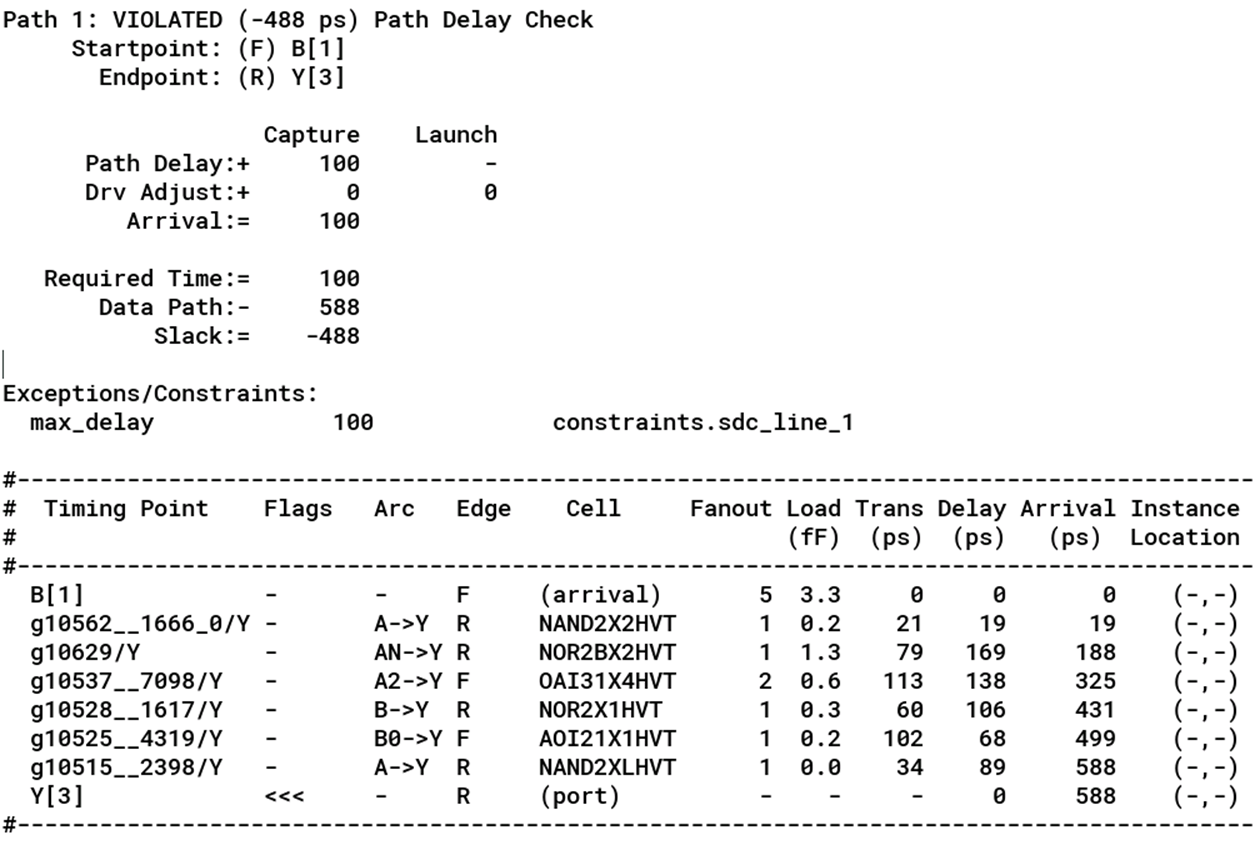
\includegraphics[width=0.8\linewidth]{figure/exp1_path1_report_corner3.png}
    \caption{Chi tiết báo cáo thời gian của đường truyền tới hạn (Path 1) tại góc Slow 1.0V HVT} %[cite: 3]
    \label{fig:exp1_c3_path1_report}
\end{figure}

Đường truyền bắt đầu từ ngõ vào \texttt{B[1]} và kết thúc tại ngõ ra \texttt{Y[3]}. %[cite: 3]
\begin{itemize}
    \item \textbf{Đường đi tín hiệu:} B[1] $\rightarrow$ NAND2X2HVT $\rightarrow$ NOR2BX2HVT $\rightarrow$ OAI31X4HVT $\rightarrow$ NOR2X1HVT $\rightarrow$ AOI21X1HVT $\rightarrow$ NAND2XLHVT $\rightarrow$ Y[3]. %[cite: 3]
    \item \textbf{Độ trễ đường truyền:} 588 ps. %[cite: 3]
    \item \textbf{Thời gian yêu cầu:} 100 ps. %[cite: 3]
    \item \textbf{Thời gian dư (Slack):} 100 ps - 588 ps = -488 ps (Vi phạm). %[cite: 3]
    \item \textbf{Kết luận:} Với Slack âm rất lớn (-488 ps), đường truyền này vi phạm nghiêm trọng yêu cầu về thời gian đã đặt ra. %[cite: 3]
\end{itemize}

\begin{figure}[H]
    \centering
    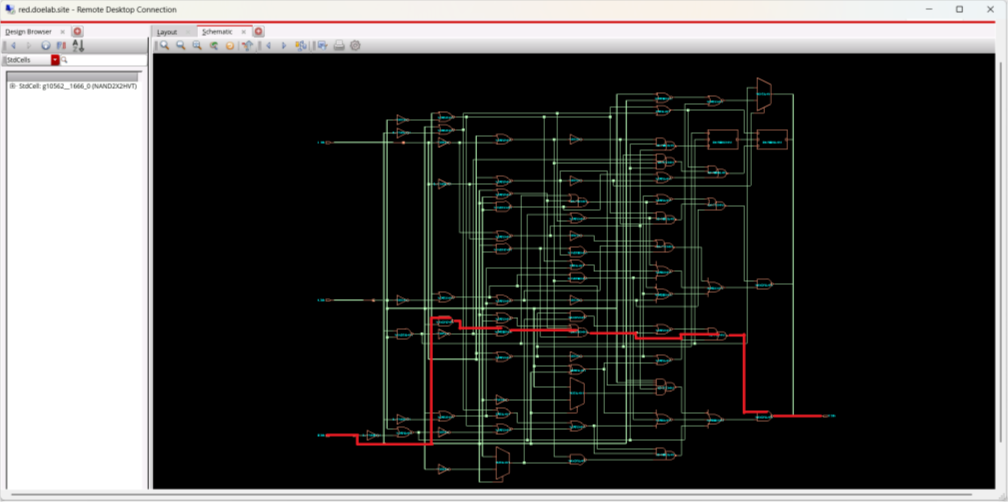
\includegraphics[width=0.8\linewidth]{figure/exp1_path1_schematic_corner3.png}
    \caption{Sơ đồ mạch hiển thị đường truyền tới hạn (Path 1) tại góc Slow 1.0V HVT} %[cite: 3]
    \label{fig:exp1_c3_path1_schematic}
\end{figure}

\textbf{B. Chi tiết báo cáo các đường truyền khác (Từ 2 đến 10)} \\
Tại điều kiện vận hành xấu nhất này, toàn bộ 9 đường truyền có độ trễ cao tiếp theo đều vi phạm nghiêm trọng giới hạn thời gian (Violated). Dưới đây là kết quả chi tiết trích xuất từ công cụ: %[cite: 3]

\begin{figure}[H]
    \centering
    \begin{minipage}{0.48\textwidth}
        \centering
        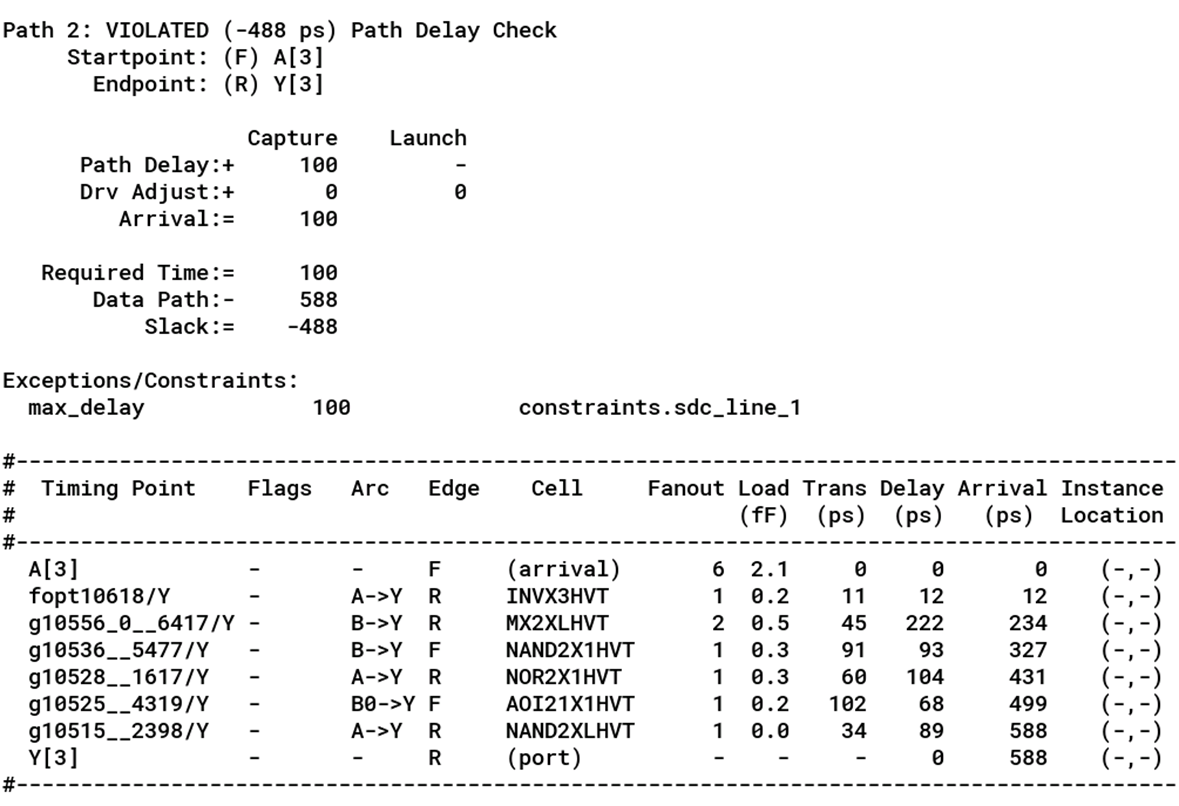
\includegraphics[width=\linewidth]{figure/exp1_path2_report_corner3.png}
        \caption{Báo cáo thời gian Path 2} %[cite: 3]
    \end{minipage}\hfill
    \begin{minipage}{0.48\textwidth}
        \centering
        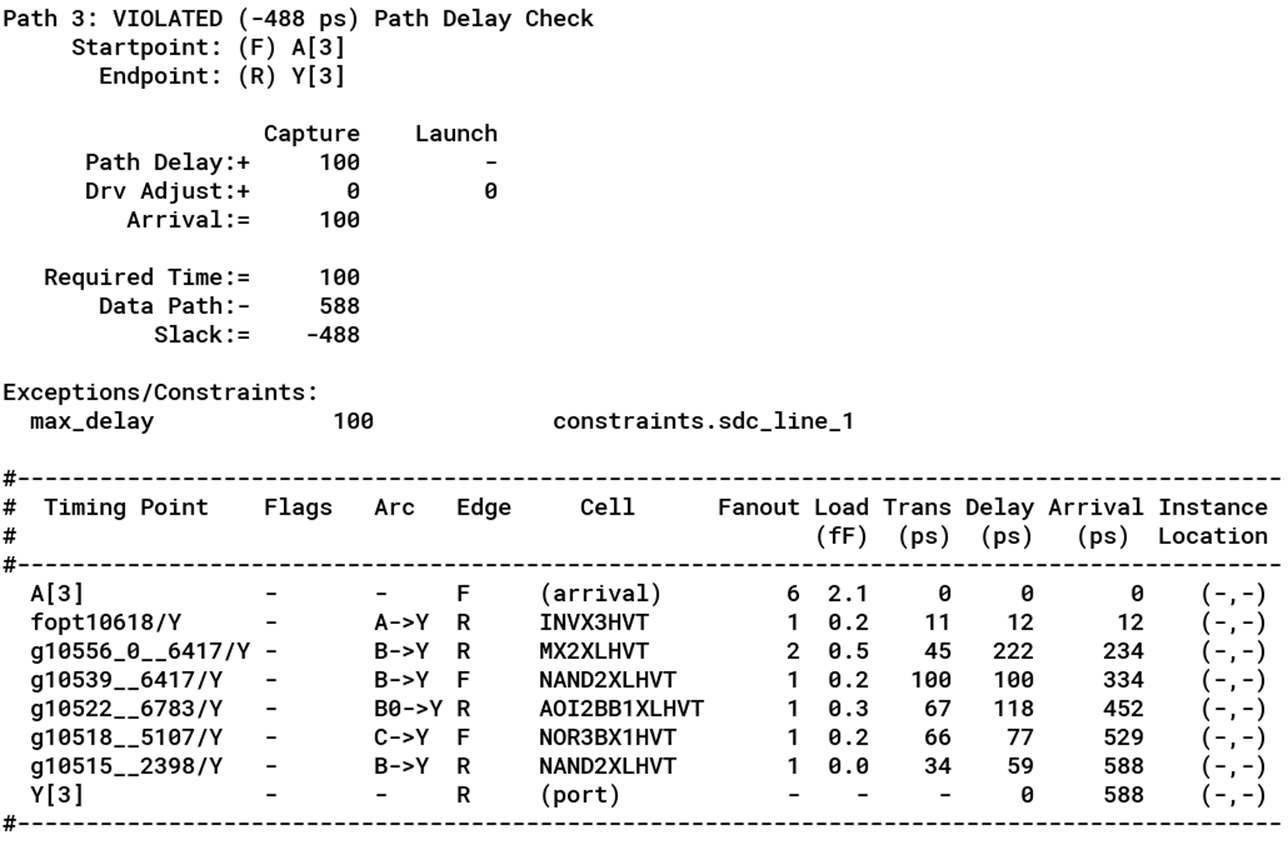
\includegraphics[width=\linewidth]{figure/exp1_path3_report_corner3.png}
        \caption{Báo cáo thời gian Path 3} %[cite: 3]
    \end{minipage}
\end{figure}

\begin{figure}[H]
    \centering
    \begin{minipage}{0.48\textwidth}
        \centering
        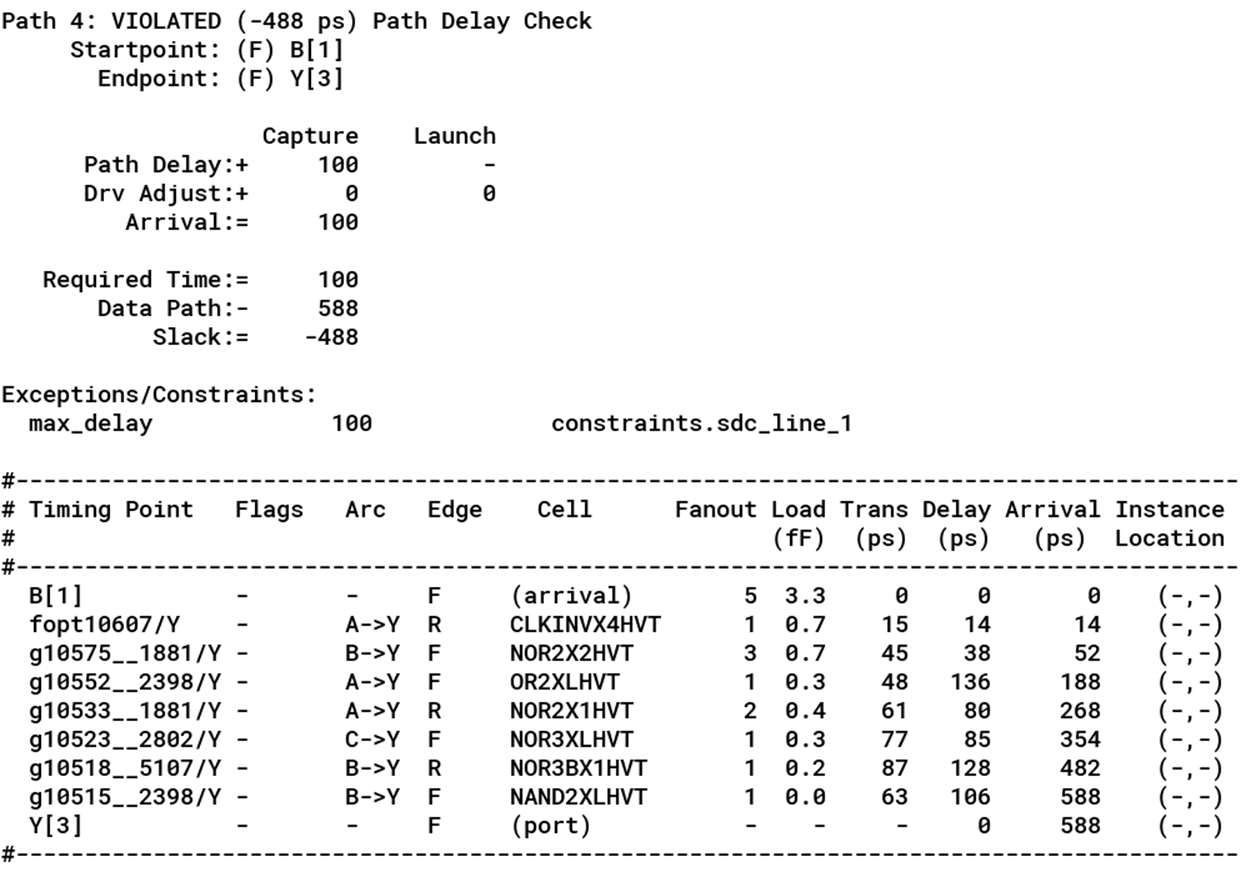
\includegraphics[width=\linewidth]{figure/exp1_path4_report_corner3.png}
        \caption{Báo cáo thời gian Path 4} %[cite: 3]
    \end{minipage}\hfill
    \begin{minipage}{0.48\textwidth}
        \centering
        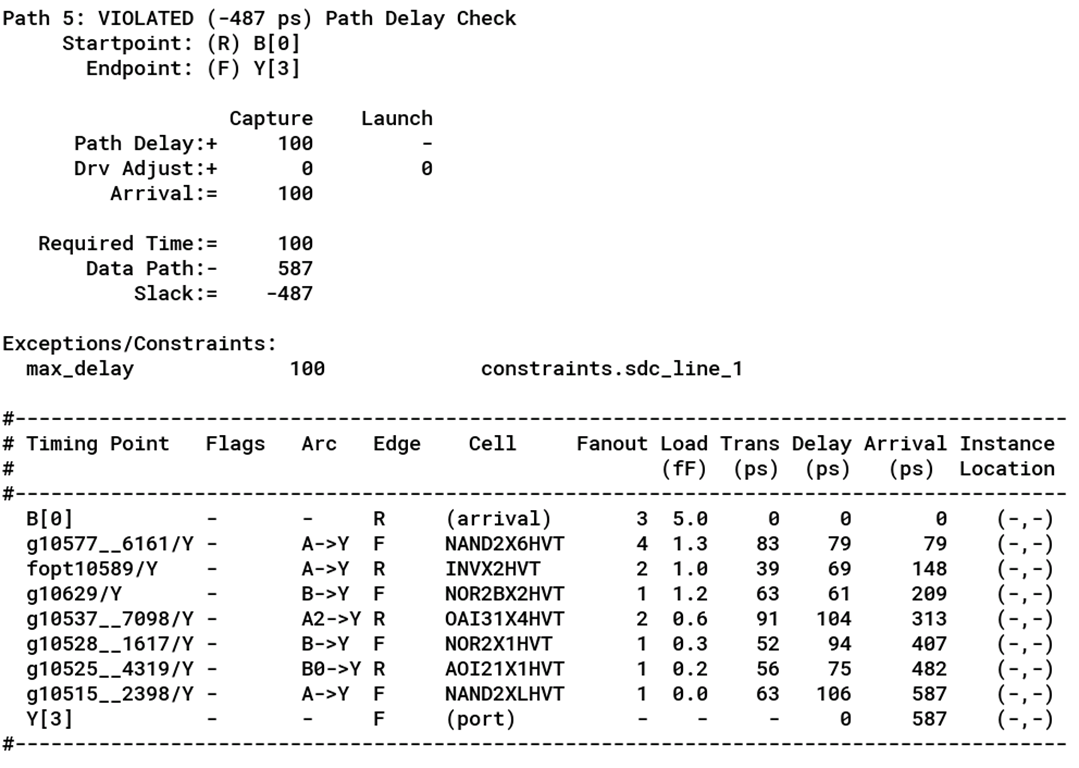
\includegraphics[width=\linewidth]{figure/exp1_path5_report_corner3.png}
        \caption{Báo cáo thời gian Path 5} %[cite: 3]
    \end{minipage}
\end{figure}

\begin{figure}[H]
    \centering
    \begin{minipage}{0.48\textwidth}
        \centering
        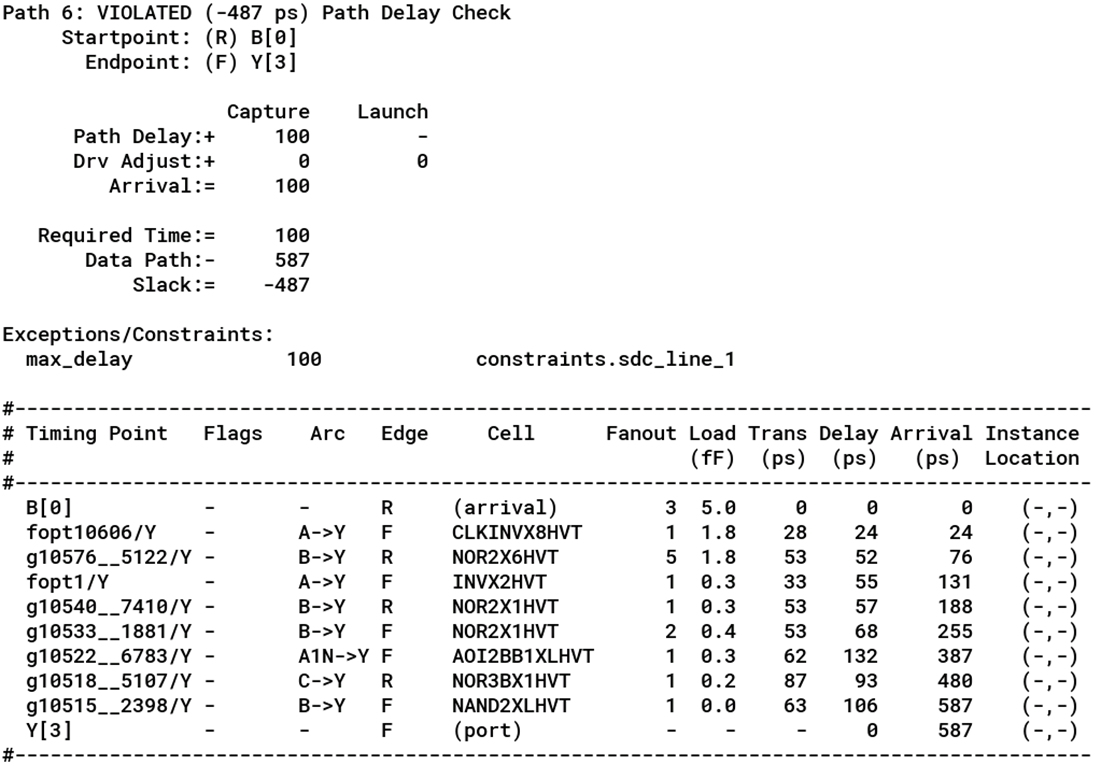
\includegraphics[width=\linewidth]{figure/exp1_path6_report_corner3.png}
        \caption{Báo cáo thời gian Path 6} %[cite: 3]
    \end{minipage}\hfill
    \begin{minipage}{0.48\textwidth}
        \centering
        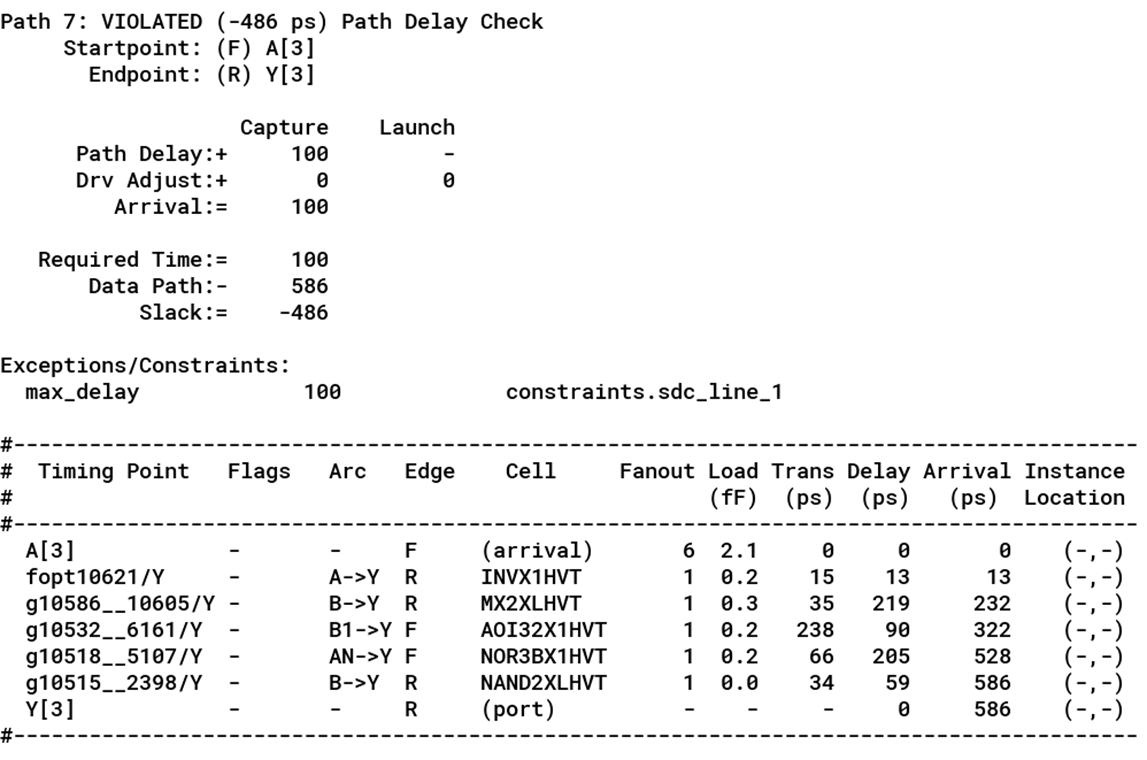
\includegraphics[width=\linewidth]{figure/exp1_path7_report_corner3.png}
        \caption{Báo cáo thời gian Path 7} %[cite: 3]
    \end{minipage}
\end{figure}

\begin{figure}[H]
    \centering
    \begin{minipage}{0.48\textwidth}
        \centering
        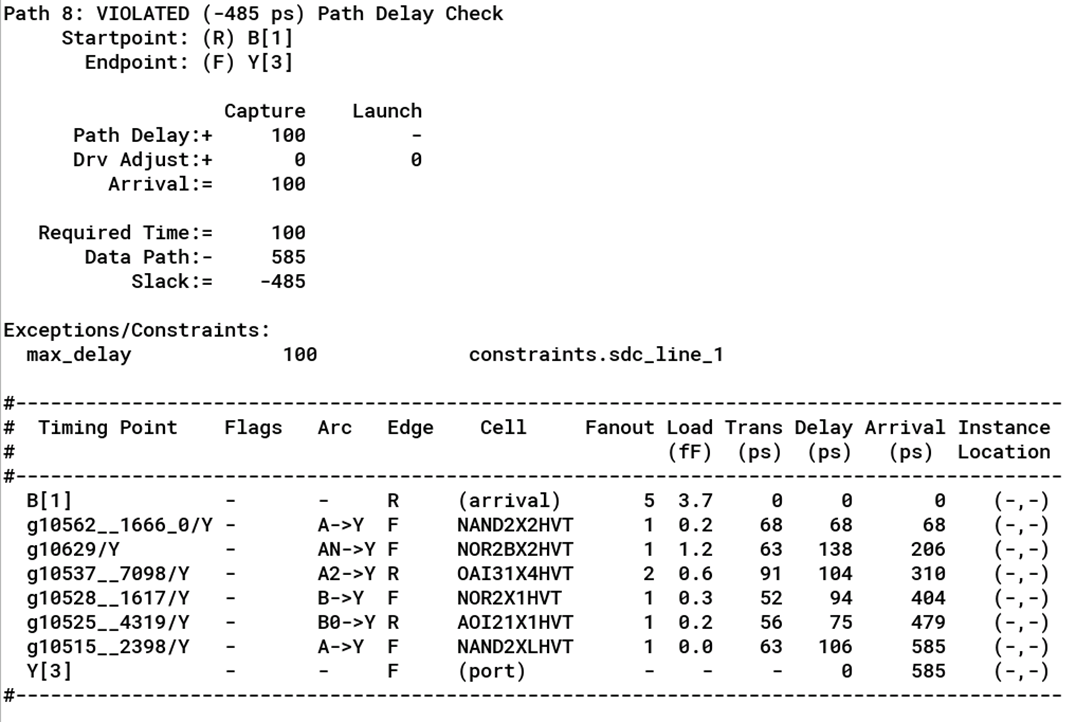
\includegraphics[width=\linewidth]{figure/exp1_path8_report_corner3.png}
        \caption{Báo cáo thời gian Path 8} %[cite: 3]
    \end{minipage}\hfill
    \begin{minipage}{0.48\textwidth}
        \centering
        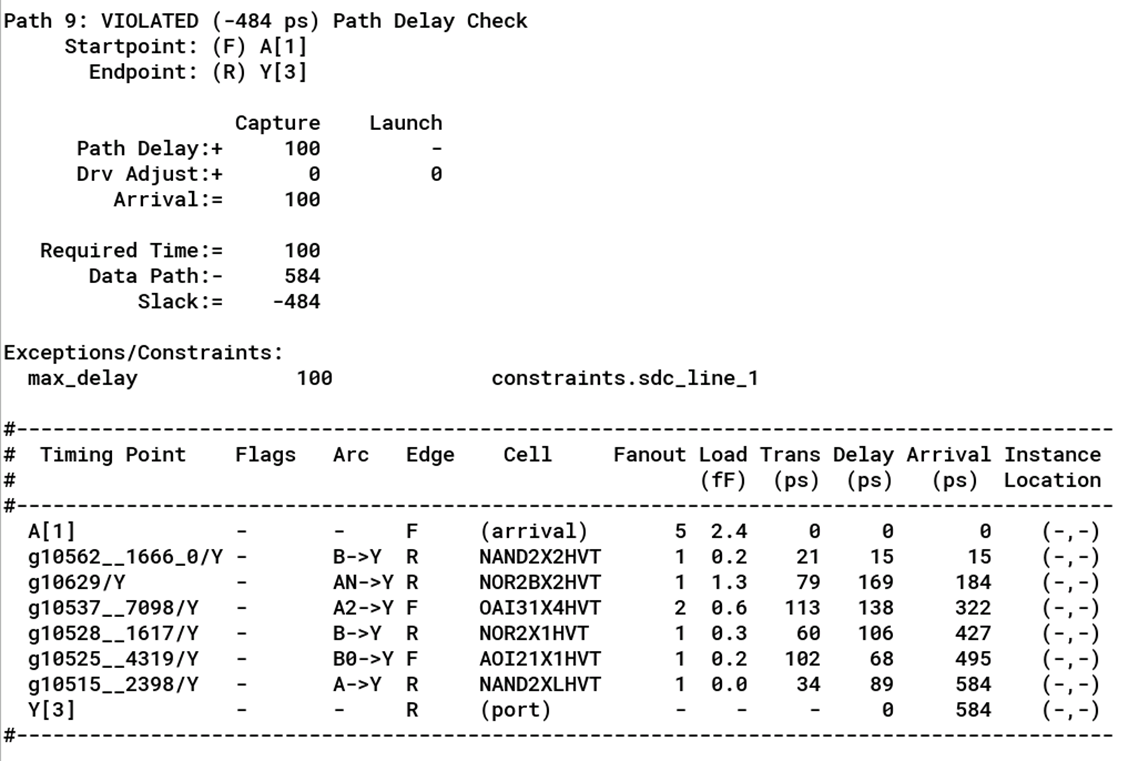
\includegraphics[width=\linewidth]{figure/exp1_path9_report_corner3.png}
        \caption{Báo cáo thời gian Path 9} %[cite: 3]
    \end{minipage}
\end{figure}

\begin{figure}[H]
    \centering
    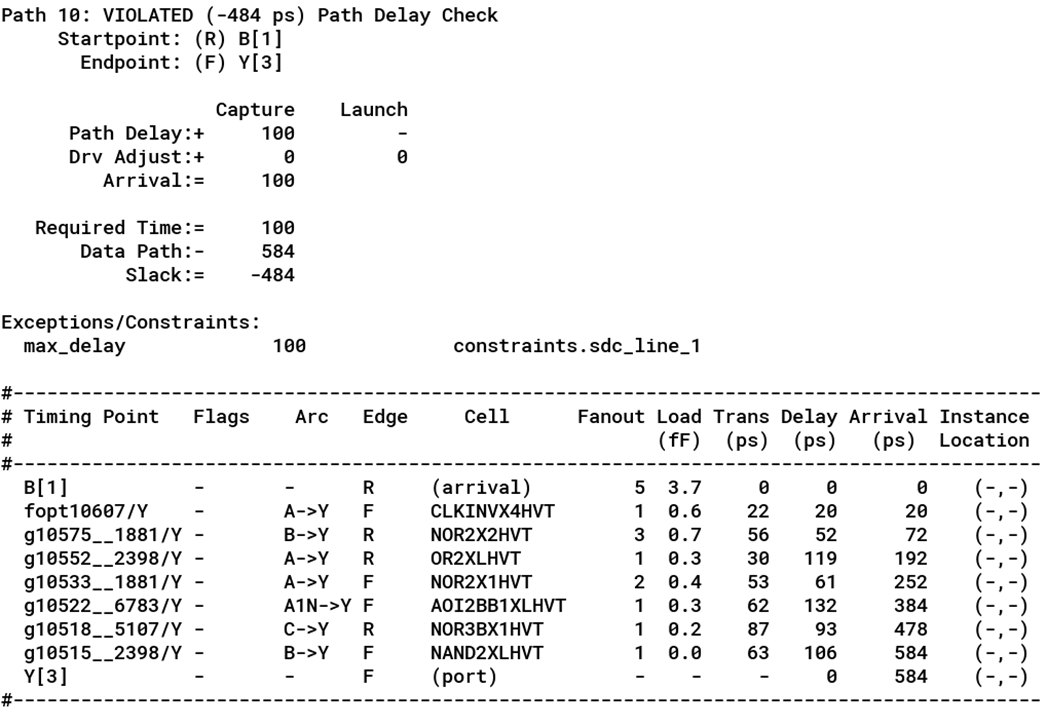
\includegraphics[width=0.48\linewidth]{figure/exp1_path10_report_corner3.png}
    \caption{Báo cáo thời gian Path 10} %[cite: 3]
    \label{fig:exp1_c3_path10}
\end{figure}

\textbf{C. Bảng tổng hợp 10 đường truyền trễ nhất}
\begin{table}[H]
    \centering
    \resizebox{\textwidth}{!}{
    \begin{tabular}{|c|p{12.5cm}|c|c|}
        \hline
        \textbf{STT} & \textbf{Đường đi tín hiệu} & \textbf{Độ trễ (ps)} & \textbf{Thời gian dư (ps)} \\
        \hline
        1 & B[1] $\rightarrow$ NAND2X2HVT $\rightarrow$ NOR2BX2HVT $\rightarrow$ OAI31X4HVT $\rightarrow$ NOR2X1HVT $\rightarrow$ AOI21X1HVT $\rightarrow$ NAND2XLHVT $\rightarrow$ Y[3] & 588 & -488 (Vi phạm) \\ \hline %[cite: 3]
        2 & A[3] $\rightarrow$ INVX3HVT $\rightarrow$ MX2XLHVT $\rightarrow$ NAND2X1HVT $\rightarrow$ NOR2X1HVT $\rightarrow$ AOI21X1HVT $\rightarrow$ NAND2XLHVT $\rightarrow$ Y[3] & 588 & -488 (Vi phạm) \\ \hline %[cite: 3]
        3 & A[3] $\rightarrow$ INVX3HVT $\rightarrow$ MX2XLHVT $\rightarrow$ NAND2XLHVT $\rightarrow$ AOI2BBXLHVT $\rightarrow$ NOR3BX1HVT $\rightarrow$ NAND2XLHVT $\rightarrow$ Y[3] & 588 & -488 (Vi phạm) \\ \hline %[cite: 3]
        4 & B[1] $\rightarrow$ CLKINVX4HVT $\rightarrow$ NOR2X2HVT $\rightarrow$ OR2XLHVT $\rightarrow$ NOR2X1HVT $\rightarrow$ NOR3XLHVT $\rightarrow$ NOR3BX1HVT $\rightarrow$ NAND2XLHVT $\rightarrow$ Y[3] & 588 & -488 (Vi phạm) \\ \hline %[cite: 3]
        5 & B[0] $\rightarrow$ NAND2X6HVT $\rightarrow$ INVX2HVT $\rightarrow$ NOR2BX2HVT $\rightarrow$ OAI31X4HVT $\rightarrow$ NOR2X1HVT $\rightarrow$ AOI21X1HVT $\rightarrow$ NAND2XLHVT $\rightarrow$ Y[3] & 587 & -487 (Vi phạm) \\ \hline %[cite: 3]
        6 & B[0] $\rightarrow$ CLKINVX8HVT $\rightarrow$ NOR2X6HVT $\rightarrow$ INVX2HVT $\rightarrow$ NOR2X1HVT $\rightarrow$ NOR2X1HVT $\rightarrow$ AOI2BB1XLHVT $\rightarrow$ NOR3BX1HVT $\rightarrow$ NAND2XLHVT $\rightarrow$ Y[3] & 587 & -487 (Vi phạm) \\ \hline %[cite: 3]
        7 & A[3] $\rightarrow$ INVX1HVT $\rightarrow$ MX2XLHVT $\rightarrow$ AOI32X1HVT $\rightarrow$ NOR3BX1HVT $\rightarrow$ NAND2XLHVT $\rightarrow$ Y[3] & 586 & -486 (Vi phạm) \\ \hline %[cite: 3]
        8 & B[1] $\rightarrow$ NAND2X2HVT $\rightarrow$ NOR2BX2HVT $\rightarrow$ OAI31X4HVT $\rightarrow$ NOR2X1HVT $\rightarrow$ AOI21X1HVT $\rightarrow$ NAND2XLHVT $\rightarrow$ Y[3] & 585 & -485 (Vi phạm) \\ \hline %[cite: 3]
        9 & A[1] $\rightarrow$ NAND2X2HVT $\rightarrow$ NOR2BX2HVT $\rightarrow$ OAI31X4HVT $\rightarrow$ NOR2X1HVT $\rightarrow$ AOI21X1HVT $\rightarrow$ NAND2XLHVT $\rightarrow$ Y[3] & 584 & -484 (Vi phạm) \\ \hline %[cite: 3]
        10 & B[1] $\rightarrow$ CLKINVX4HVT $\rightarrow$ NOR2X2HVT $\rightarrow$ OR2XLHVT $\rightarrow$ NOR2X1HVT $\rightarrow$ AOI2BB1XLHVT $\rightarrow$ NOR3BX1HVT $\rightarrow$ NAND2XLHVT $\rightarrow$ Y[3] & 584 & -484 (Vi phạm) \\ \hline %[cite: 3]
    \end{tabular}
    }
    \caption{Tổng hợp 10 đường truyền trễ nhất - Góc Chậm 1.0V HVT}
\end{table}

\textbf{D. Nhận xét phân tích} \\
Khác biệt hoàn toàn so với góc Fast 1.2V, tại điều kiện quy trình chế tạo xấu nhất (Slow - SS) kết hợp với mức điện áp cung cấp giảm sâu chỉ còn 1.0V, thời gian trễ của đường dẫn tới hạn đã tăng vọt lên tới 588 ps. Sự suy giảm điện áp dẫn đến hiện tượng "đói dòng" (dòng điện bão hòa suy yếu) kết hợp với điện áp ngưỡng $V_{th}$ vốn đã cao của thư viện HVT, khiến mạch xử lý rất chậm. Với yêu cầu \texttt{max\_delay} là 100 ps, hệ thống vi phạm timing một cách nghiêm trọng với Slack âm lên đến -488 ps, chứng tỏ việc sử dụng cấu hình này hoàn toàn không khả thi cho xung nhịp hiện tại. %[cite: 3]

% ================= CORNER 4 =================
\subsubsection{Corner 4: Chậm (SS) - 1.2V - HVT (\texttt{slow\_vdd1v2\_basicCells\_hvt.lib})}

\textbf{A. Phân tích đường truyền tới hạn (Đường truyền số 1)} \\
Dựa trên kết quả tổng hợp và phân tích STA ở điều kiện quy trình Chậm (Slow) nhưng với điện áp danh định 1.2V, đường truyền có độ trễ lớn nhất được xác định với các thông số như sau: %[cite: 3]

\begin{figure}[H]
    \centering
    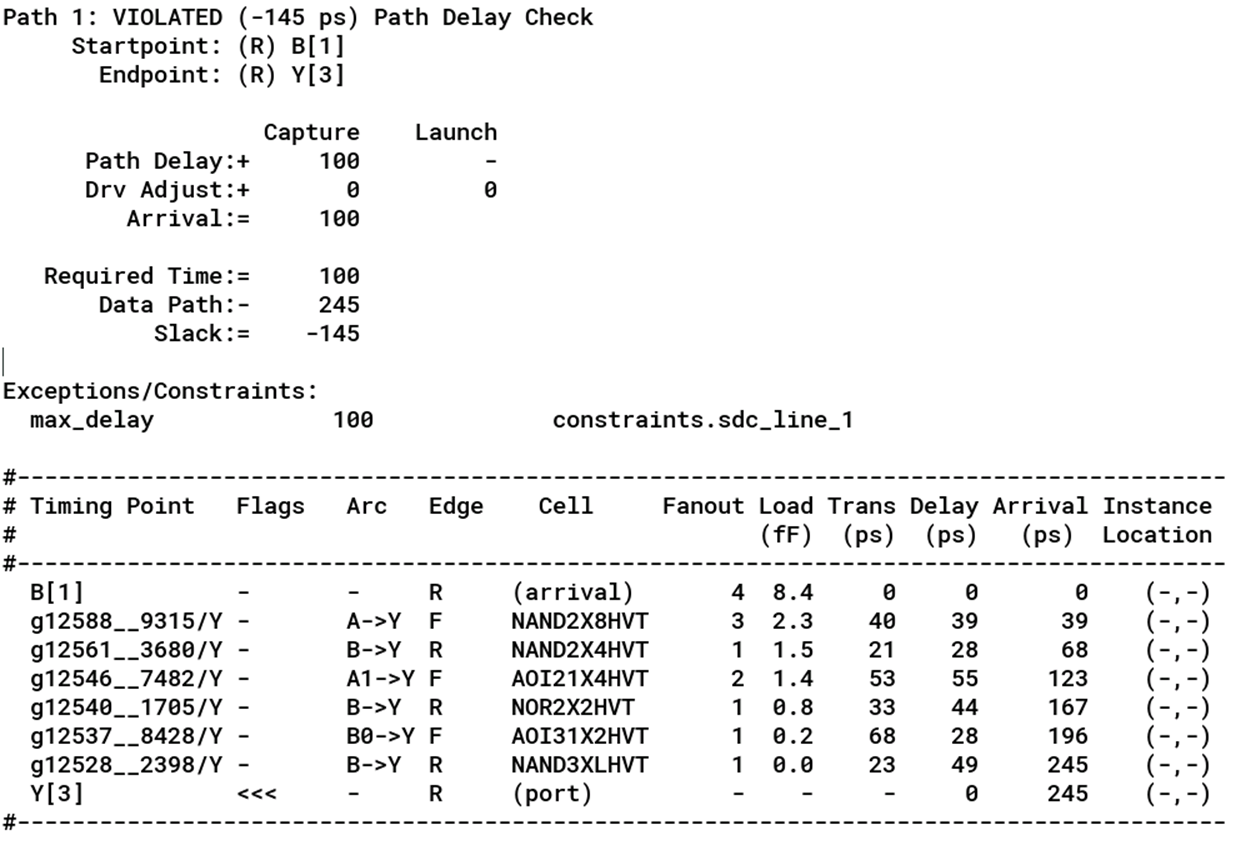
\includegraphics[width=0.8\linewidth]{figure/exp1_path1_report_corner4.png}
    \caption{Chi tiết báo cáo thời gian của đường truyền tới hạn (Path 1) tại góc Slow 1.2V HVT} %[cite: 3]
    \label{fig:exp1_c4_path1_report}
\end{figure}

Đường truyền bắt đầu từ ngõ vào \texttt{B[1]} và kết thúc tại ngõ ra \texttt{Y[3]}. %[cite: 3]
\begin{itemize}
    \item \textbf{Đường đi tín hiệu:} B[1] $\rightarrow$ NAND2X8HVT $\rightarrow$ NAND2X4HVT $\rightarrow$ AOI21X4HVT $\rightarrow$ NOR2X2HVT $\rightarrow$ AOI31X2HVT $\rightarrow$ NAND3XLHVT $\rightarrow$ Y[3]. %[cite: 3]
    \item \textbf{Độ trễ đường truyền:} 245 ps. %[cite: 3]
    \item \textbf{Thời gian yêu cầu:} 100 ps. %[cite: 3]
    \item \textbf{Thời gian dư (Slack):} 100 ps - 245 ps = -145 ps (Vi phạm). %[cite: 3]
    \item \textbf{Kết luận:} Với Slack âm (-145 ps), đường truyền này vẫn vi phạm yêu cầu về thời gian đã đặt ra, dù mức độ vi phạm đã giảm so với góc 1.0V. %[cite: 3]
\end{itemize}

\begin{figure}[H]
    \centering
    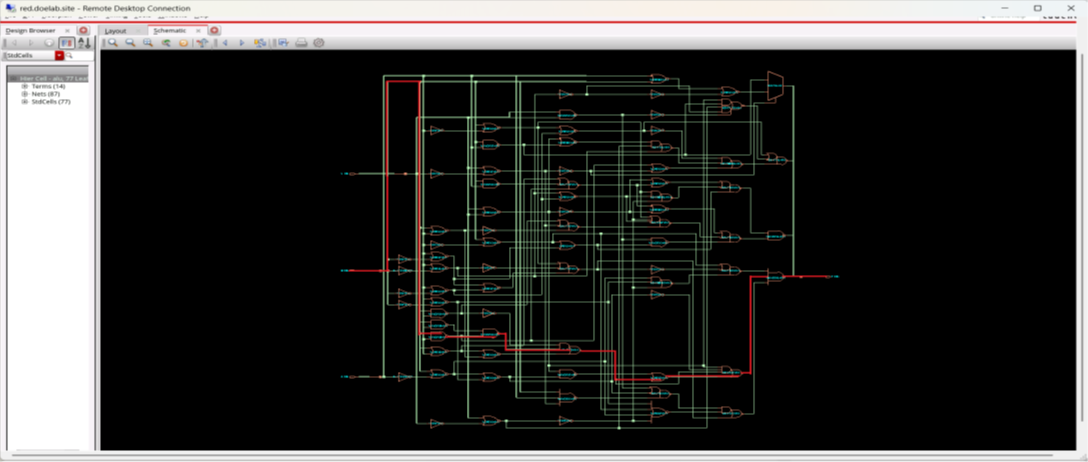
\includegraphics[width=0.8\linewidth]{figure/exp1_path1_schematic_corner4.png}
    \caption{Sơ đồ mạch hiển thị đường truyền tới hạn (Path 1) tại góc Slow 1.2V HVT} %[cite: 3]
    \label{fig:exp1_c4_path1_schematic}
\end{figure}

\textbf{B. Chi tiết báo cáo các đường truyền khác (Từ 2 đến 10)} \\
Tại điều kiện vận hành này, toàn bộ 9 đường truyền có độ trễ cao tiếp theo cũng đều ghi nhận tình trạng vi phạm giới hạn thời gian (Violated). Dưới đây là kết quả chi tiết trích xuất từ công cụ: %[cite: 3]

\begin{figure}[H]
    \centering
    \begin{minipage}{0.48\textwidth}
        \centering
        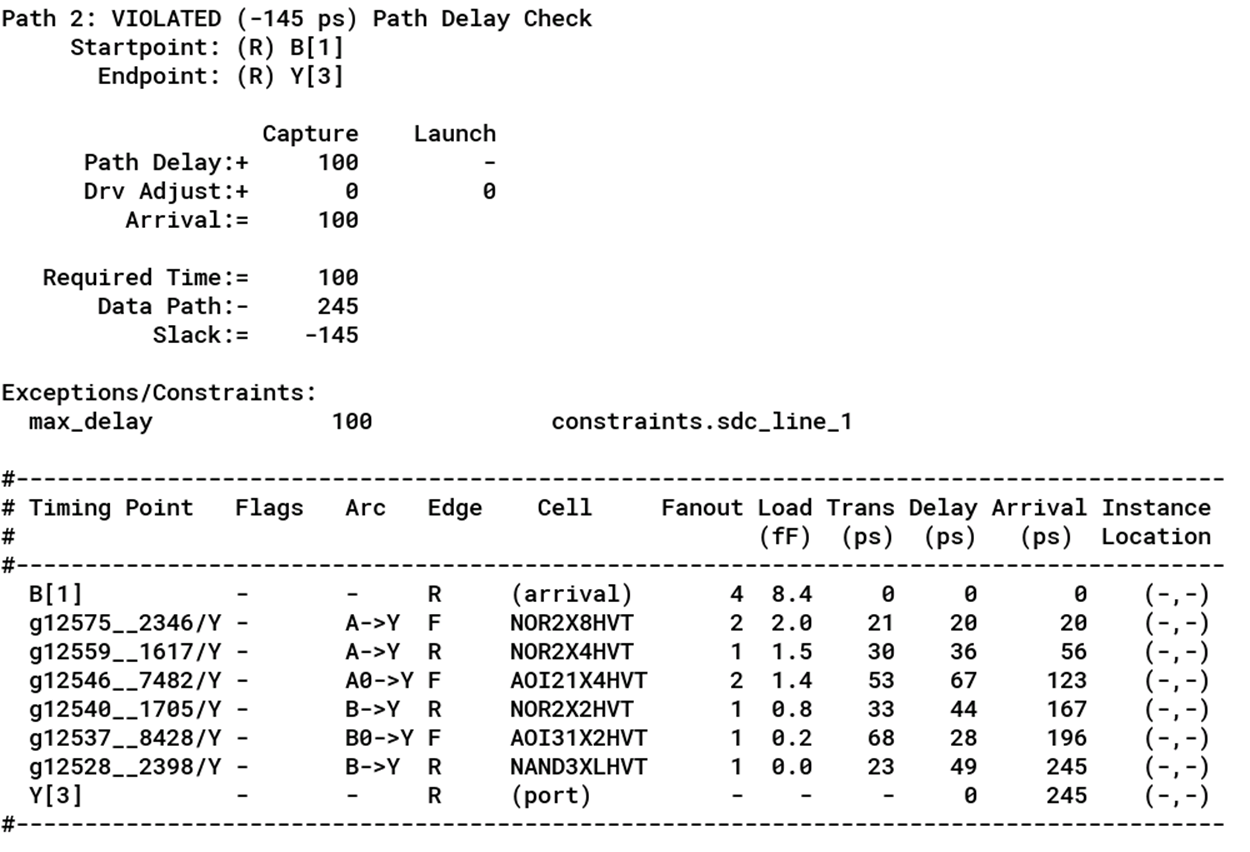
\includegraphics[width=\linewidth]{figure/exp1_path2_report_corner4.png}
        \caption{Báo cáo thời gian Path 2} %[cite: 3]
    \end{minipage}\hfill
    \begin{minipage}{0.48\textwidth}
        \centering
        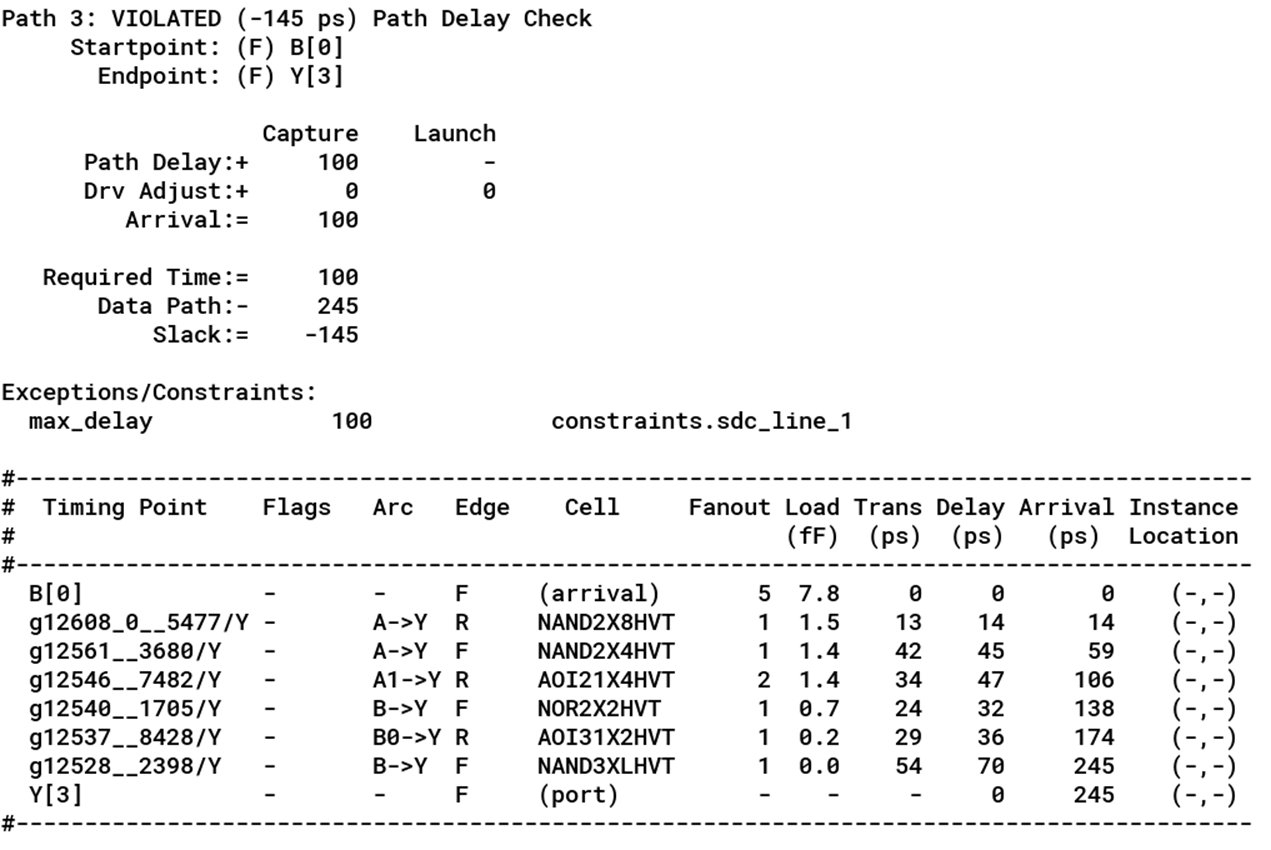
\includegraphics[width=\linewidth]{figure/exp1_path3_report_corner4.png}
        \caption{Báo cáo thời gian Path 3} %[cite: 3]
    \end{minipage}
\end{figure}

\begin{figure}[H]
    \centering
    \begin{minipage}{0.48\textwidth}
        \centering
        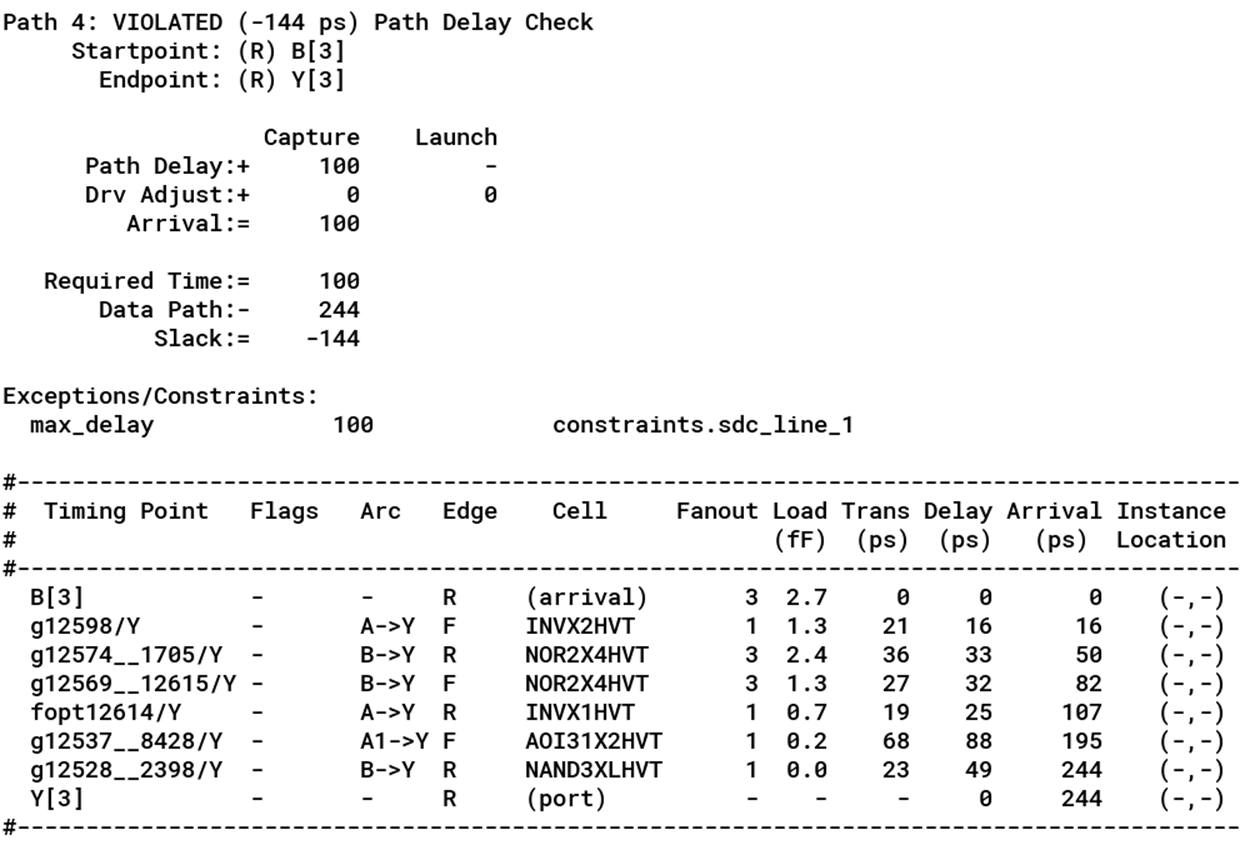
\includegraphics[width=\linewidth]{figure/exp1_path4_report_corner4.png}
        \caption{Báo cáo thời gian Path 4} %[cite: 3]
    \end{minipage}\hfill
    \begin{minipage}{0.48\textwidth}
        \centering
        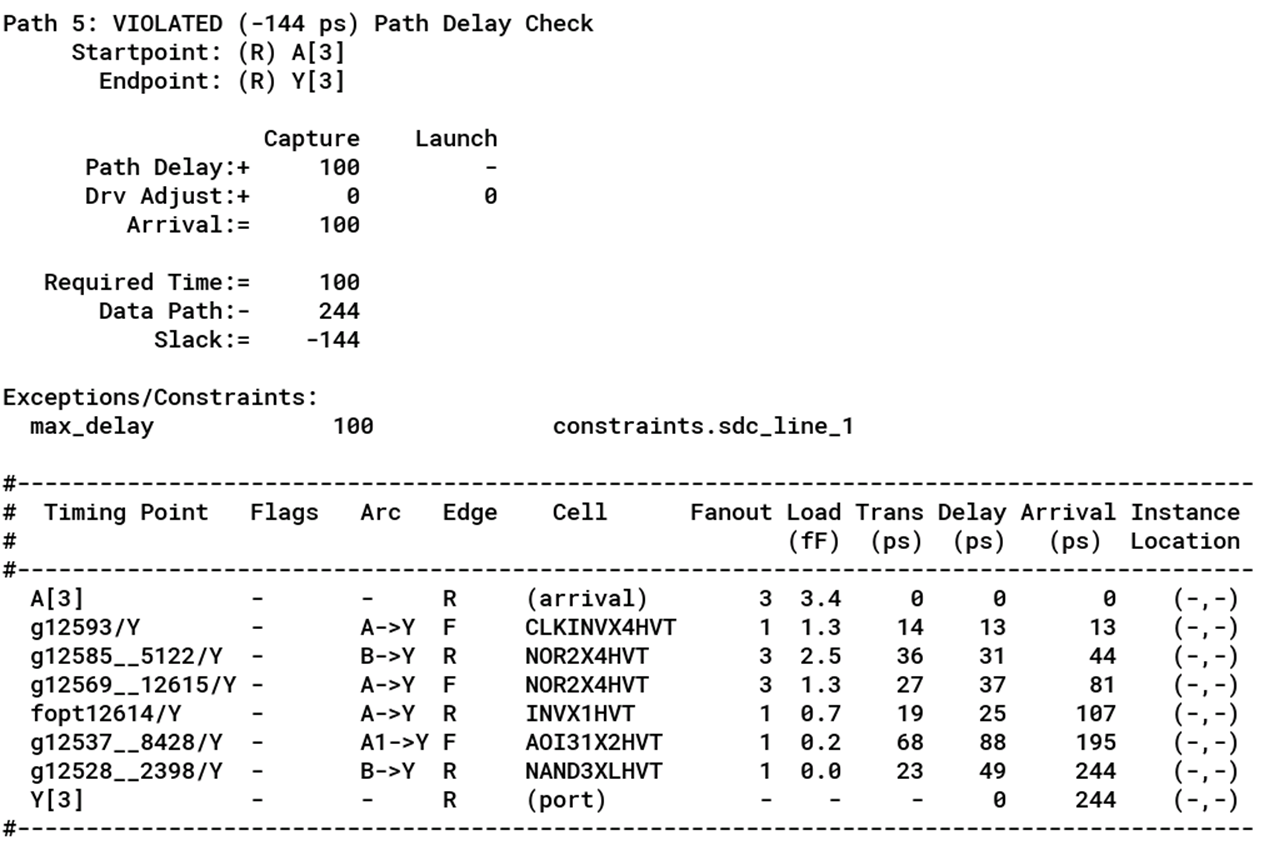
\includegraphics[width=\linewidth]{figure/exp1_path5_report_corner4.png}
        \caption{Báo cáo thời gian Path 5} %[cite: 3]
    \end{minipage}
\end{figure}

\begin{figure}[H]
    \centering
    \begin{minipage}{0.48\textwidth}
        \centering
        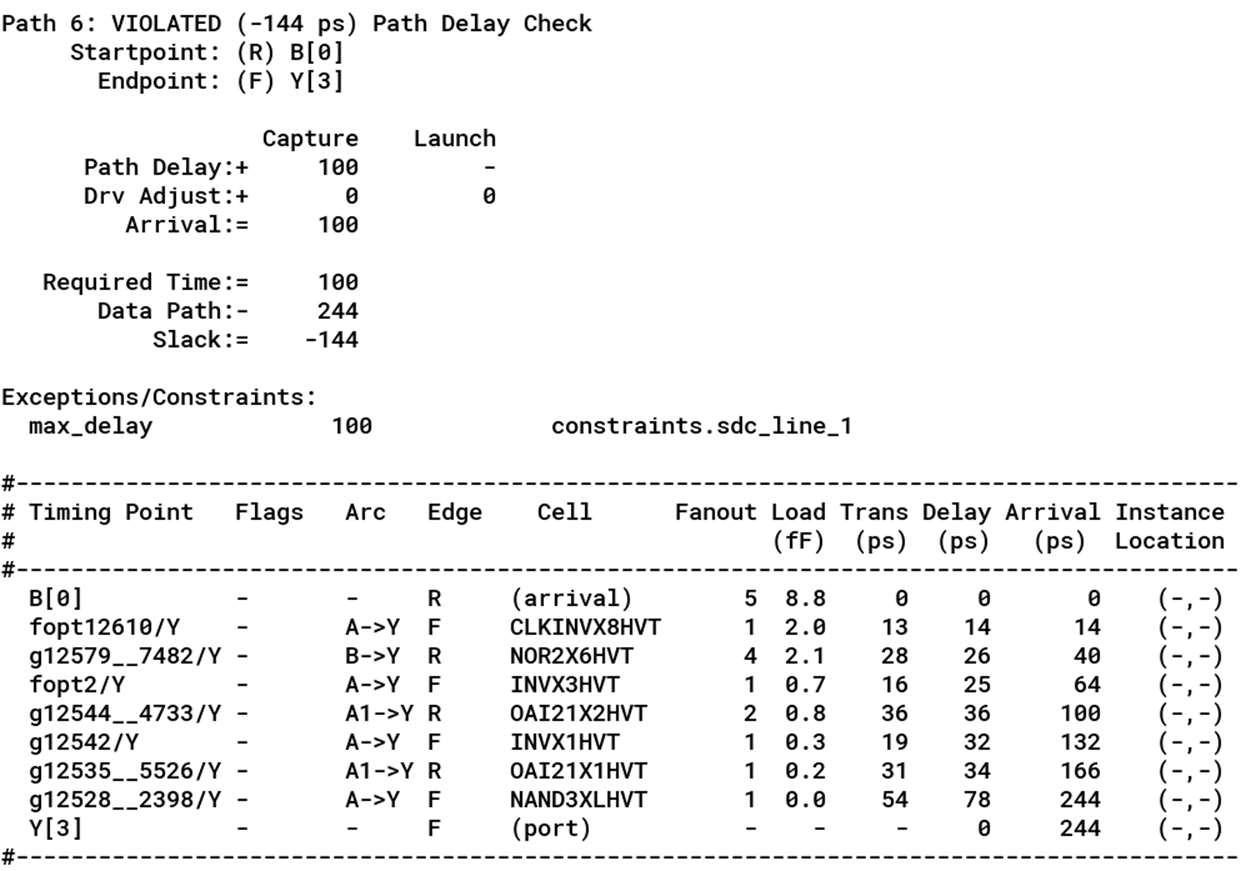
\includegraphics[width=\linewidth]{figure/exp1_path6_report_corner4.png}
        \caption{Báo cáo thời gian Path 6} %[cite: 3]
    \end{minipage}\hfill
    \begin{minipage}{0.48\textwidth}
        \centering
        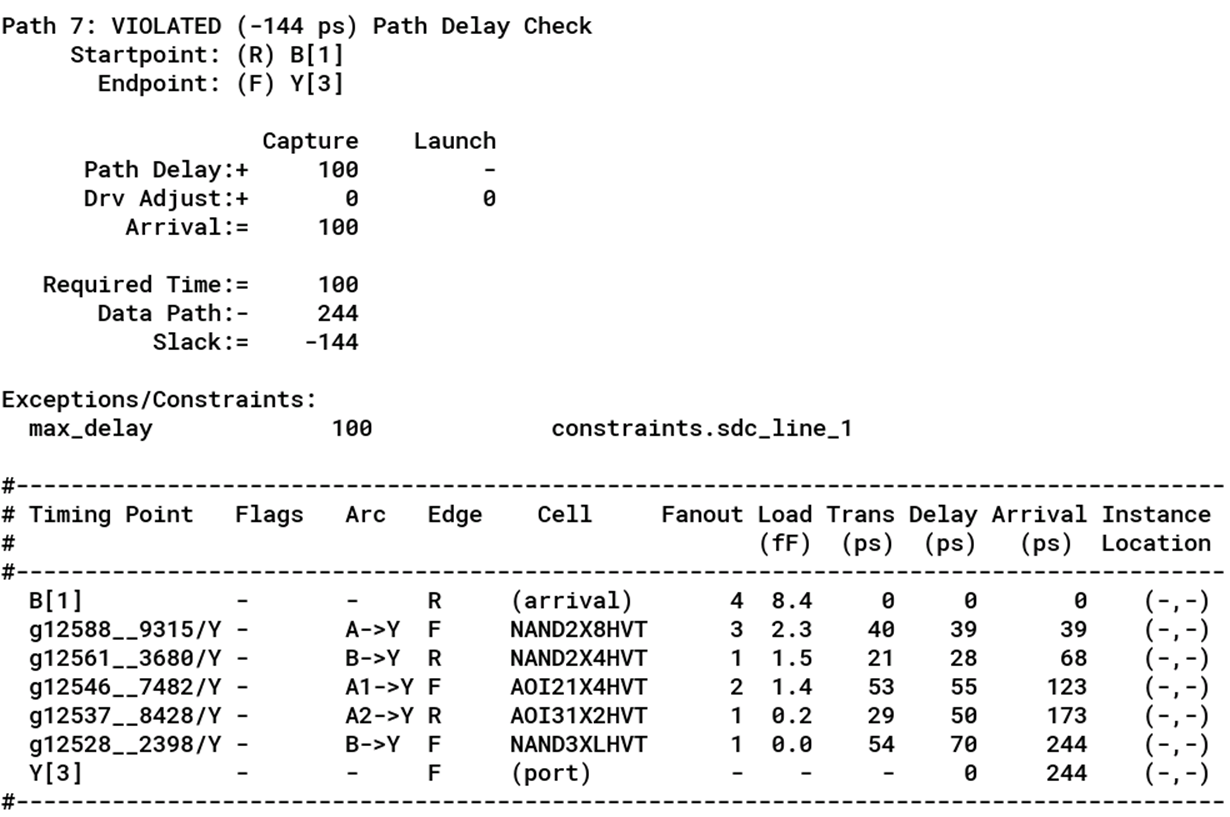
\includegraphics[width=\linewidth]{figure/exp1_path7_report_corner4.png}
        \caption{Báo cáo thời gian Path 7} %[cite: 3]
    \end{minipage}
\end{figure}

\begin{figure}[H]
    \centering
    \begin{minipage}{0.48\textwidth}
        \centering
        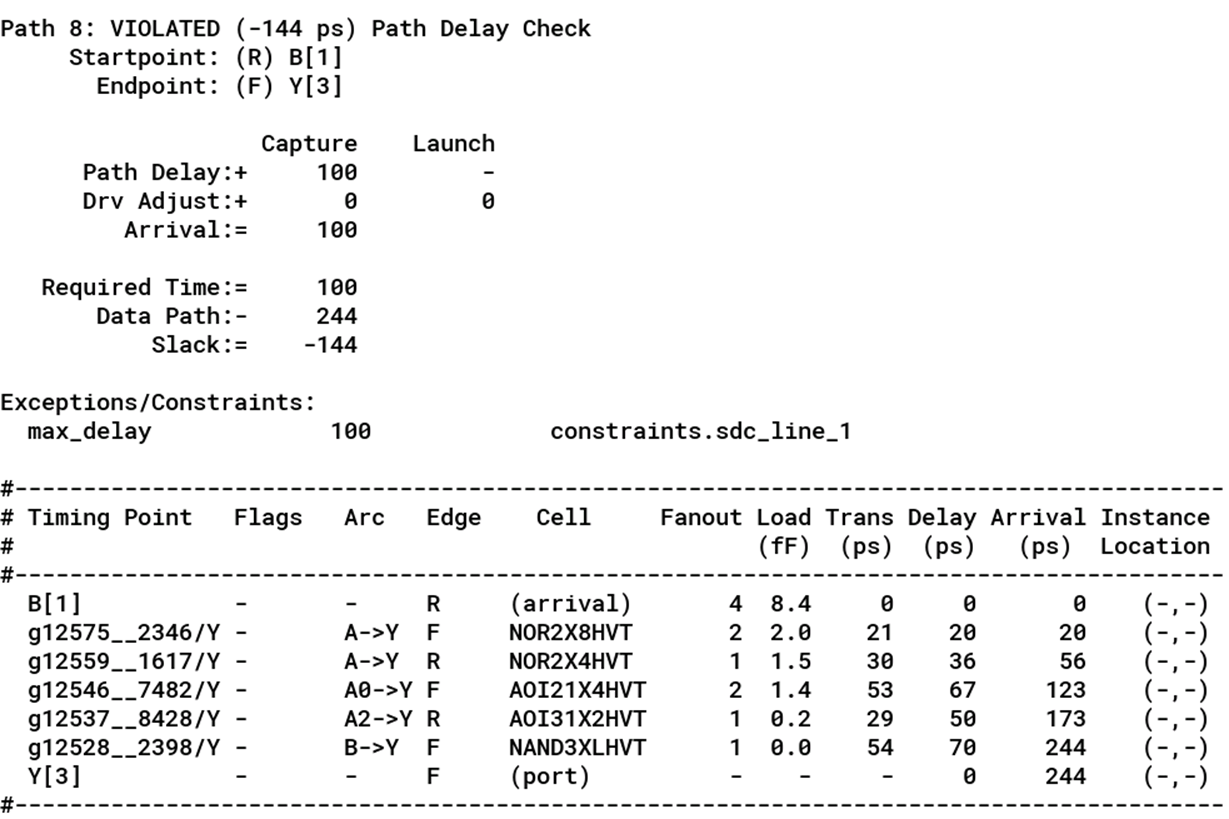
\includegraphics[width=\linewidth]{figure/exp1_path8_report_corner4.png}
        \caption{Báo cáo thời gian Path 8} %[cite: 3]
    \end{minipage}\hfill
    \begin{minipage}{0.48\textwidth}
        \centering
        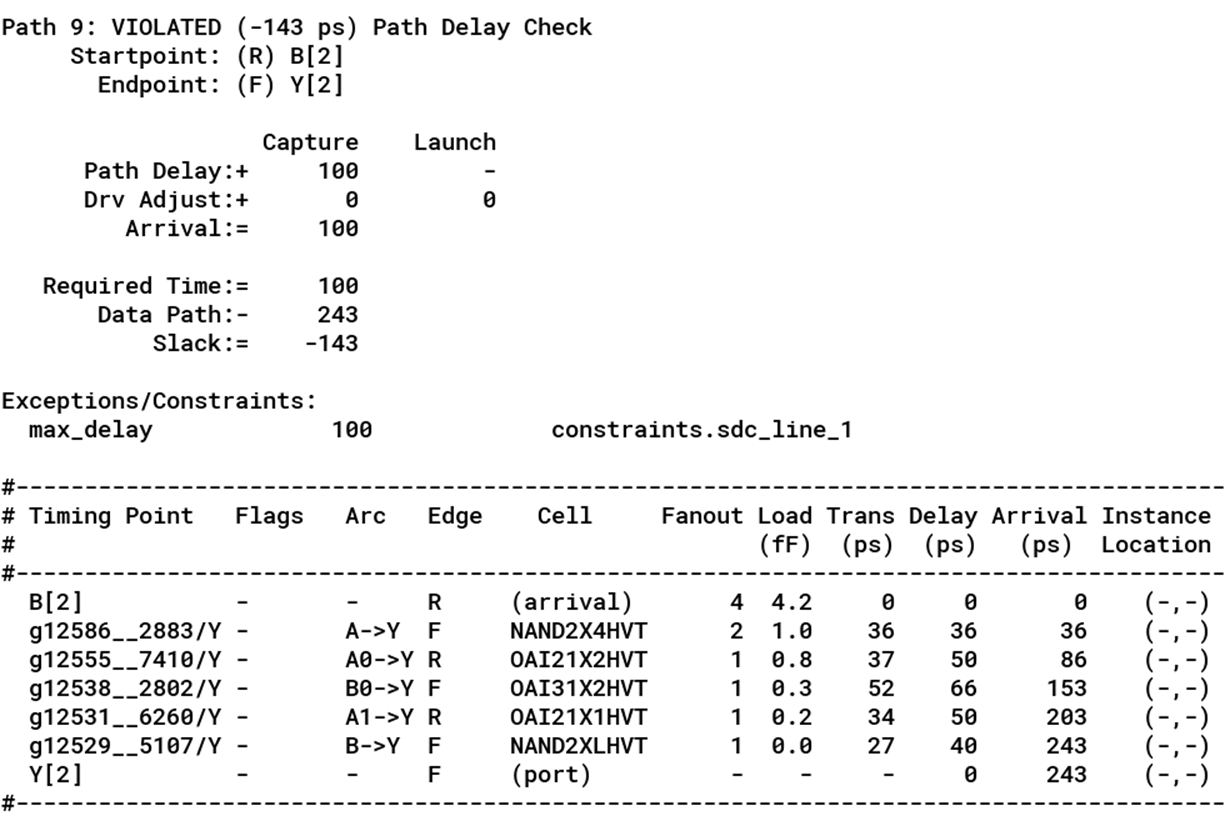
\includegraphics[width=\linewidth]{figure/exp1_path9_report_corner4.png}
        \caption{Báo cáo thời gian Path 9} %[cite: 3]
    \end{minipage}
\end{figure}

\begin{figure}[H]
    \centering
    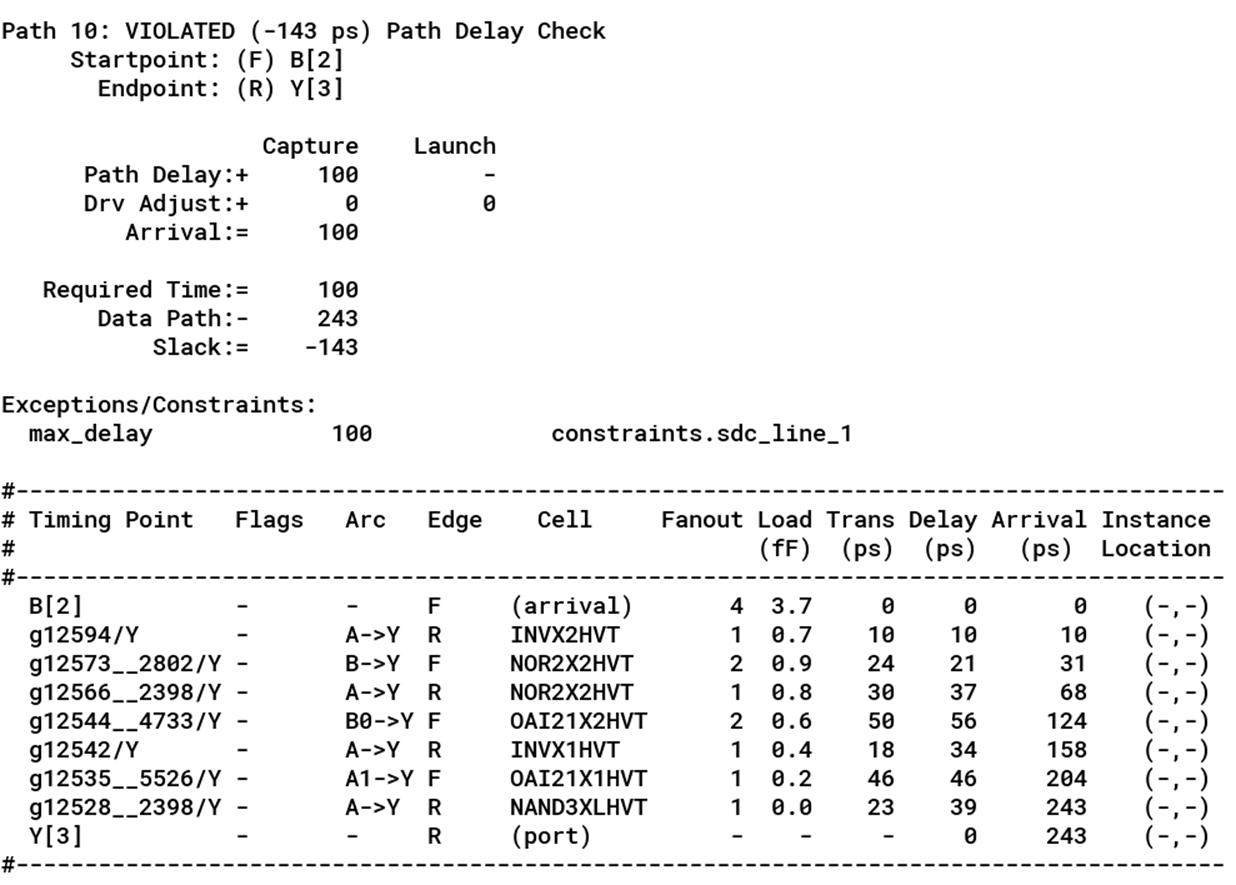
\includegraphics[width=0.48\linewidth]{figure/exp1_path10_report_corner4.png}
    \caption{Báo cáo thời gian Path 10} %[cite: 3]
    \label{fig:exp1_c4_path10}
\end{figure}

\textbf{C. Bảng tổng hợp 10 đường truyền trễ nhất}
\begin{table}[H]
    \centering
    \resizebox{\textwidth}{!}{
    \begin{tabular}{|c|p{12.5cm}|c|c|}
        \hline
        \textbf{STT} & \textbf{Đường đi tín hiệu} & \textbf{Độ trễ (ps)} & \textbf{Thời gian dư (ps)} \\
        \hline
        1 & B[1] $\rightarrow$ NAND2X8HVT $\rightarrow$ NAND2X4HVT $\rightarrow$ AOI21X4HVT $\rightarrow$ NOR2X2HVT $\rightarrow$ AOI31X2HVT $\rightarrow$ NAND3XLHVT $\rightarrow$ Y[3] & 245 & -145 (Vi phạm) \\ \hline %[cite: 3]
        2 & B[1] $\rightarrow$ NOR2X8HVT $\rightarrow$ NOR2X4HVT $\rightarrow$ AOI21X4HVT $\rightarrow$ NOR2X2HVT $\rightarrow$ AOI31X2HVT $\rightarrow$ NAND3XLHVT $\rightarrow$ Y[3] & 245 & -145 (Vi phạm) \\ \hline %[cite: 3]
        3 & B[0] $\rightarrow$ NAND2X8HVT $\rightarrow$ NAND2X4HVT $\rightarrow$ AOI21X4HVT $\rightarrow$ NOR2X2HVT $\rightarrow$ AOI31X2HVT $\rightarrow$ NAND3XLHVT $\rightarrow$ Y[3] & 245 & -145 (Vi phạm) \\ \hline %[cite: 3]
        4 & B[3] $\rightarrow$ INVX2HVT $\rightarrow$ NOR2X4HVT $\rightarrow$ NOR2X4HVT $\rightarrow$ INVX1HVT $\rightarrow$ AOI31X2HVT $\rightarrow$ NAND3XLHVT $\rightarrow$ Y[3] & 244 & -144 (Vi phạm) \\ \hline %[cite: 3]
        5 & A[3] $\rightarrow$ CLKINX4HVT $\rightarrow$ NOR2X4HVT $\rightarrow$ NOR2X4HVT $\rightarrow$ INVX1HVT $\rightarrow$ AOI31X2HVT $\rightarrow$ NAND3XLHVT $\rightarrow$ Y[3] & 244 & -144 (Vi phạm) \\ \hline %[cite: 3]
        6 & B[0] $\rightarrow$ CLKINVX8HVT $\rightarrow$ NOR2X6HVT $\rightarrow$ INVX3HVT $\rightarrow$ OAI21X2HVT $\rightarrow$ INVX1HVT $\rightarrow$ OAI21X1HVT $\rightarrow$ NAND3XLHVT $\rightarrow$ Y[3] & 244 & -144 (Vi phạm) \\ \hline %[cite: 3]
        7 & B[1] $\rightarrow$ NAND2X8HVT $\rightarrow$ NAND2X4HVT $\rightarrow$ AOI21X4HVT $\rightarrow$ AOI31X2HVT $\rightarrow$ NAND3XLHVT $\rightarrow$ Y[3] & 244 & -144 (Vi phạm) \\ \hline %[cite: 3]
        8 & B[1] $\rightarrow$ NOR2X8HVT $\rightarrow$ NOR2X4HVT $\rightarrow$ AOI21X4HVT $\rightarrow$ AOI31X2HVT $\rightarrow$ NAND3XLHVT $\rightarrow$ Y[3] & 244 & -144 (Vi phạm) \\ \hline %[cite: 3]
        9 & B[2] $\rightarrow$ NAND2X4HVT $\rightarrow$ OAI21X4HVT $\rightarrow$ OAI31X2HVT $\rightarrow$ OAI21X1HVT $\rightarrow$ NAND2XLHVT $\rightarrow$ Y[2] & 243 & -143 (Vi phạm) \\ \hline %[cite: 3]
        10 & B[2] $\rightarrow$ INVX2HVT $\rightarrow$ NOR2X2HVT $\rightarrow$ NOR2X2HVT $\rightarrow$ OAI21X2HVT $\rightarrow$ INVX1HVT $\rightarrow$ OAI21X1HVT $\rightarrow$ NAND3XLHVT $\rightarrow$ Y[3] & 243 & -143 (Vi phạm) \\ \hline %[cite: 3]
    \end{tabular}
    }
    \caption{Tổng hợp 10 đường truyền trễ nhất - Góc Chậm 1.2V HVT}
\end{table}

\textbf{D. Nhận xét phân tích} \\
Mặc dù vẫn hoạt động ở điều kiện quy trình chế tạo xấu nhất (Slow - SS), nhưng khi điện áp cung cấp được nâng từ 1.0V lên mức danh định 1.2V, hiệu suất của mạch đã được cải thiện rõ rệt. Độ trễ của đường truyền dài nhất đã giảm mạnh từ 588 ps (ở Góc 3) xuống chỉ còn 245 ps (nhanh hơn gấp đôi). Việc cung cấp đủ điện áp đã giải quyết phần lớn hiện tượng suy hao dòng điện, giúp các cell HVT chuyển mạch dứt khoát hơn. Tuy nhiên, với ràng buộc \texttt{max\_delay} quá khắt khe là 100 ps, mức độ cải thiện này vẫn chưa đủ để đưa các đường truyền về mức an toàn, dẫn đến hệ thống vẫn vi phạm timing với Slack là -145 ps. %[cite: 3]
\newpage
% --------------------------------------------------
% ================= EXPERIMENT 2 =================
\section{Experiment 2: Timing optimization under varying constraints}
\textit{Khảo sát mạch sử dụng thư viện \texttt{slow\_vdd1v2\_basicCells\_hvt.lib}.}

\subsection{Khảo sát mạch tổng hợp theo các mốc Constraint (Max Delay)}

% ---------- Max Delay = 10 ns ----------
\subsubsection{Max Delay = 10 ns}
Dựa trên kết quả tổng hợp, đường truyền có độ trễ lớn nhất được xác định như sau:

\begin{figure}[H]
    \centering
    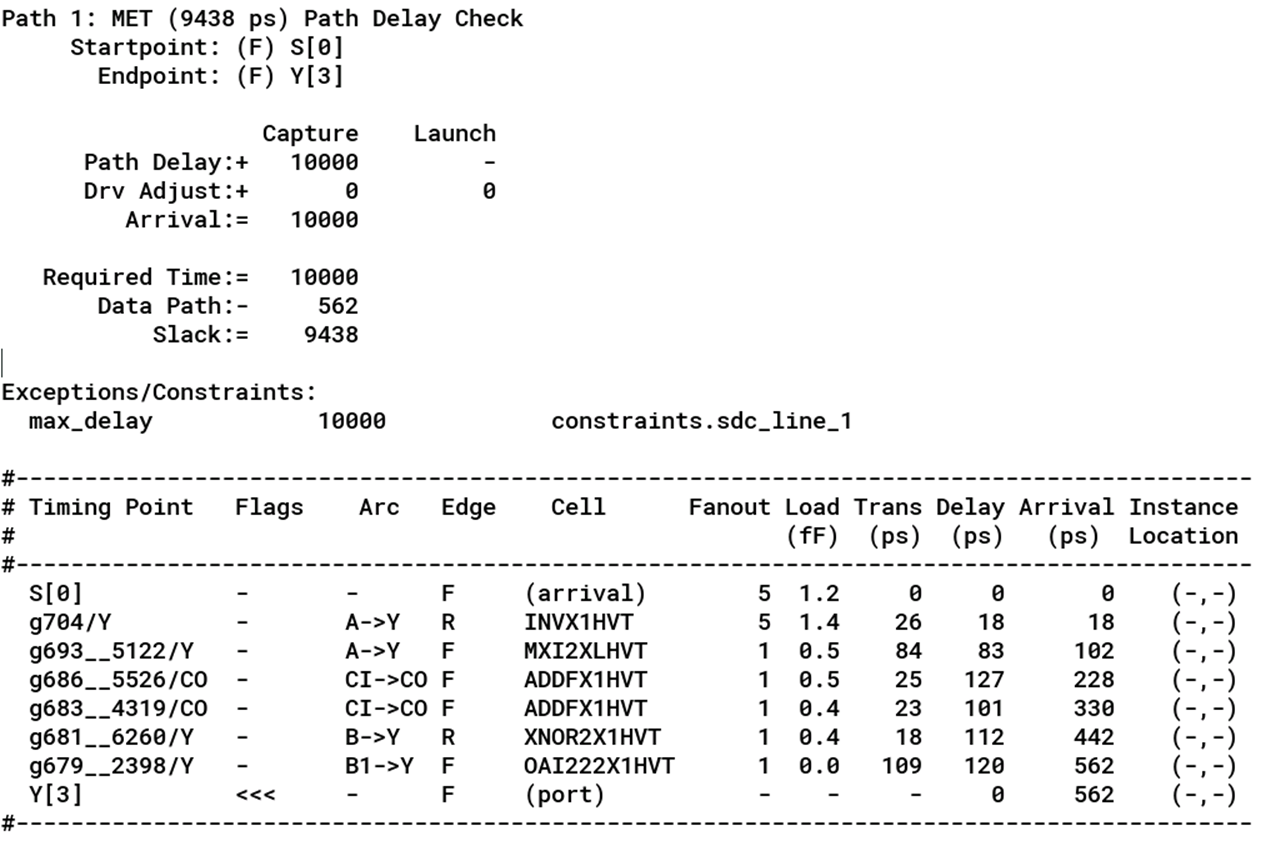
\includegraphics[width=0.8\linewidth]{figure/exp2_10ns_report.png}
    \caption{Chi tiết báo cáo thời gian tại mốc Max Delay = 10 ns}
    \label{fig:exp2_10ns_report}
\end{figure}

\begin{itemize}
    \item \textbf{Đường đi tín hiệu:} \texttt{S[0]} $\rightarrow$ INVX1HVT $\rightarrow$ MXI2XLHVT $\rightarrow$ ADDFX1HVT $\rightarrow$ ADDFX1HVT $\rightarrow$ XNOR2X1HVT $\rightarrow$ OAI222X1HVT $\rightarrow$ \texttt{Y[3]}.
    \item \textbf{Thời gian dữ liệu truyền:} 562 ps.
    \item \textbf{Thời gian yêu cầu:} 10000 ps.
    \item \textbf{Thời gian dư:} 10000 ps - 562 ps = 9438 ps (Đạt - MET).
    \item \textbf{Kết luận:} Không vi phạm Timing.
\end{itemize}

\begin{figure}[H]
    \centering
    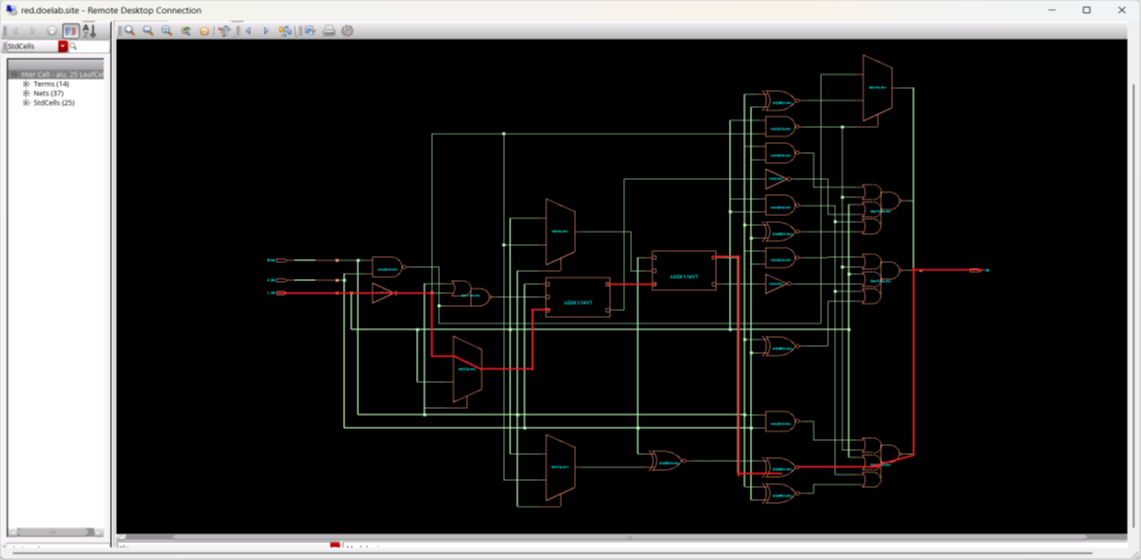
\includegraphics[width=\linewidth]{figure/exp2_10ns_schematic.png}
    \caption{Sơ đồ mạch hiển thị đường truyền tới hạn tại Max Delay = 10 ns}
    \label{fig:exp2_10ns_schematic}
\end{figure}

% ---------- Max Delay = 1 ns ----------
\subsubsection{Max Delay = 1 ns}

\begin{figure}[H]
    \centering
    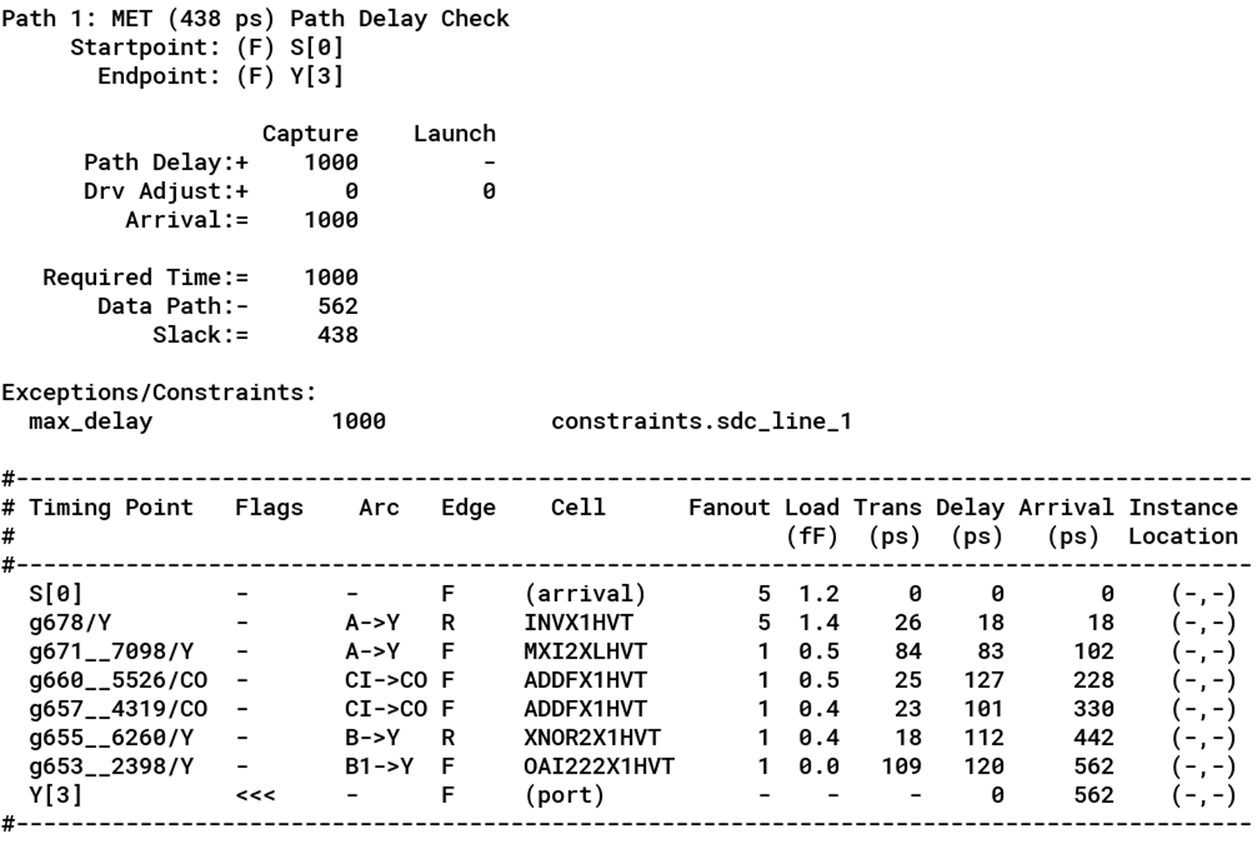
\includegraphics[width=0.8\linewidth]{figure/exp2_1ns_report.png}
    \caption{Chi tiết báo cáo thời gian tại mốc Max Delay = 1 ns}
    \label{fig:exp2_1ns_report}
\end{figure}

\begin{itemize}
    \item \textbf{Đường đi tín hiệu:} \texttt{S[0]} $\rightarrow$ INVX1HVT $\rightarrow$ MXI2XLHVT $\rightarrow$ ADDFX1HVT $\rightarrow$ ADDFX1HVT $\rightarrow$ XNOR2X1HVT $\rightarrow$ OAI222X1HVT $\rightarrow$ \texttt{Y[3]}.
    \item \textbf{Thời gian dữ liệu truyền:} 562 ps.
    \item \textbf{Thời gian yêu cầu:} 1000 ps.
    \item \textbf{Thời gian dư:} 1000 ps - 562 ps = 438 ps (Đạt - MET).
    \item \textbf{Kết luận:} Không vi phạm Timing.
\end{itemize}

\begin{figure}[H]
    \centering
    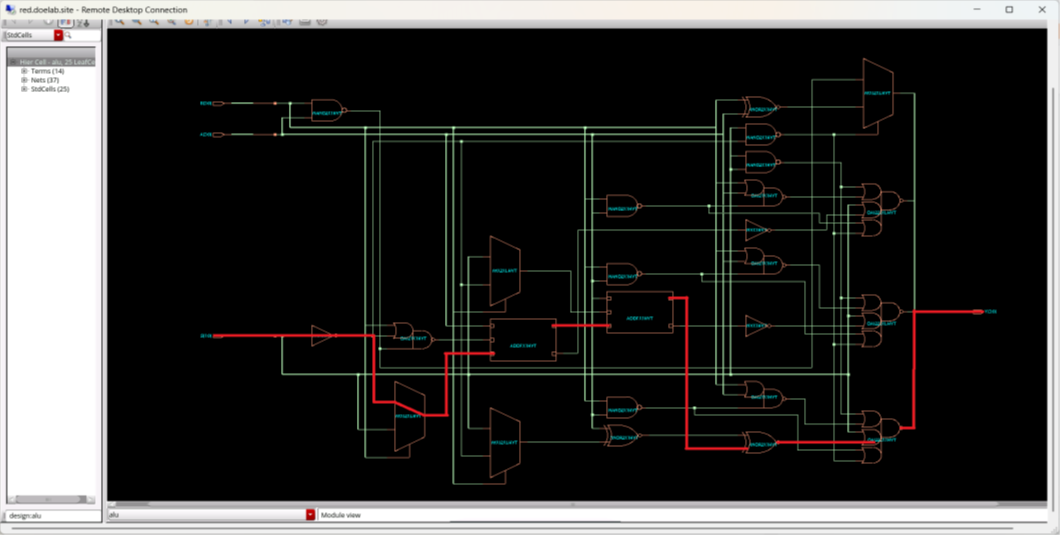
\includegraphics[width=\linewidth]{figure/exp2_1ns_schematic.png}
    \caption{Sơ đồ mạch hiển thị đường truyền tới hạn tại Max Delay = 1 ns}
    \label{fig:exp2_1ns_schematic}
\end{figure}

% ---------- Max Delay = 0.5 ns ----------
\subsubsection{Max Delay = 0.5 ns}

\begin{figure}[H]
    \centering
    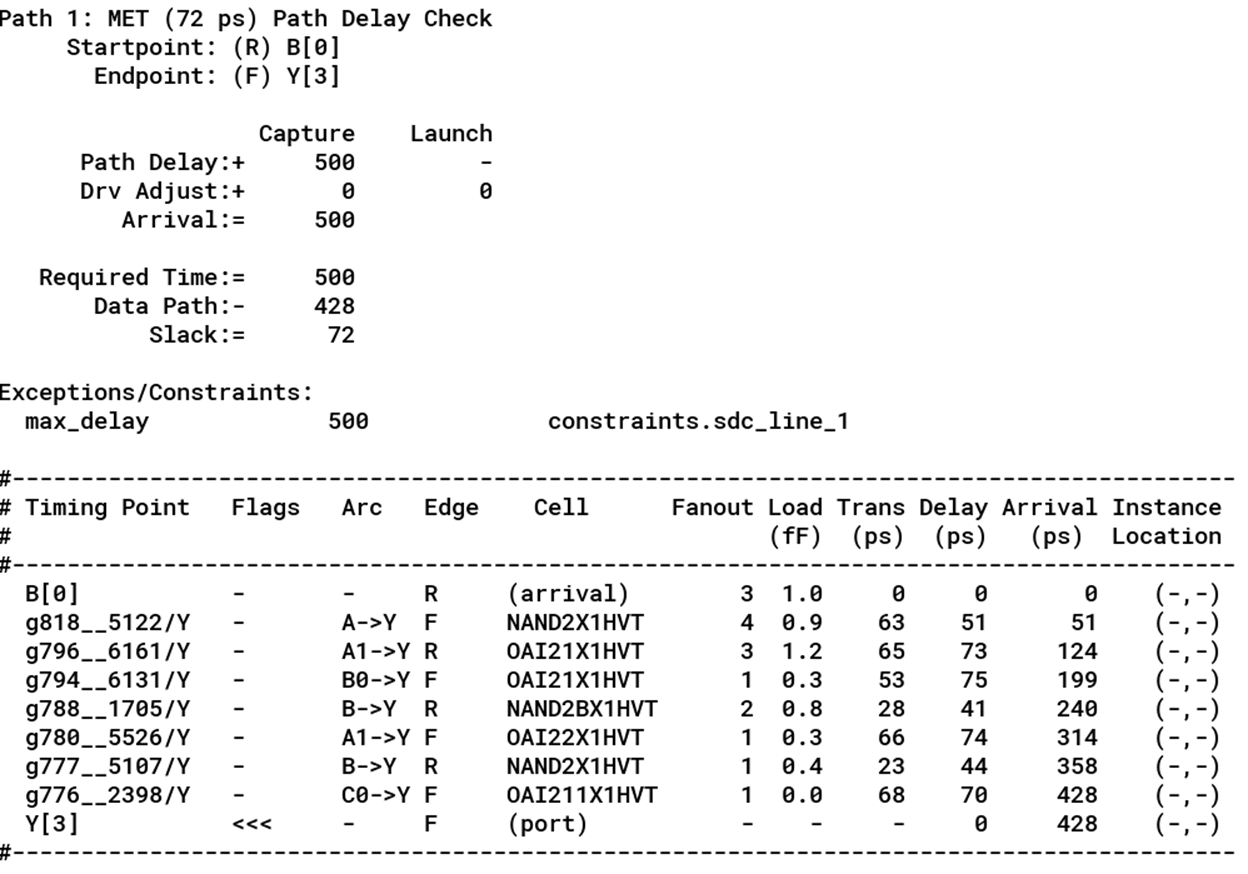
\includegraphics[width=0.8\linewidth]{figure/exp2_0.5ns_report.png}
    \caption{Chi tiết báo cáo thời gian tại mốc Max Delay = 0.5 ns}
    \label{fig:exp2_05ns_report}
\end{figure}

\begin{itemize}
    \item \textbf{Đường đi tín hiệu:} \texttt{B[0]} $\rightarrow$ NAND2X1HVT $\rightarrow$ OAI21X1HVT $\rightarrow$ OAI21X1HVT $\rightarrow$ NAND2B1HVT $\rightarrow$ OAI22X1HVT $\rightarrow$ NAND2X1HVT $\rightarrow$ OAI211X1HVT $\rightarrow$ \texttt{Y[3]}.
    \item \textbf{Thời gian dữ liệu truyền:} 428 ps.
    \item \textbf{Thời gian yêu cầu:} 500 ps.
    \item \textbf{Thời gian dư:} 500 ps - 428 ps = 72 ps (Đạt - MET).
    \item \textbf{Kết luận:} Không vi phạm Timing.
\end{itemize}

\begin{figure}[H]
    \centering
    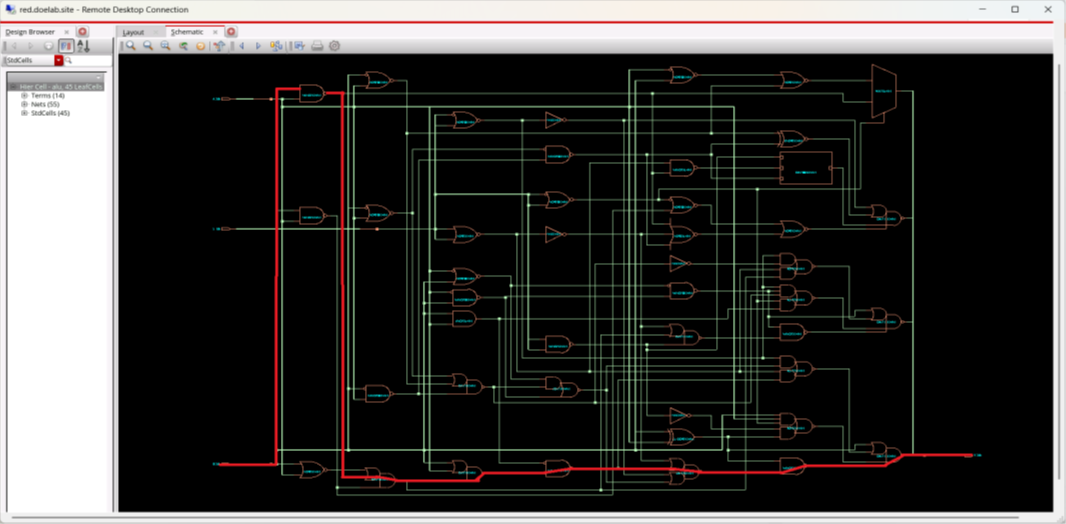
\includegraphics[width=\linewidth]{figure/exp2_0.5ns_schematic.png}
    \caption{Sơ đồ mạch hiển thị đường truyền tới hạn tại Max Delay = 0.5 ns}
    \label{fig:exp2_05ns_schematic}
\end{figure}

% ---------- Max Delay = 0.2 ns ----------
\subsubsection{Max Delay = 0.2 ns}

\begin{figure}[H]
    \centering
    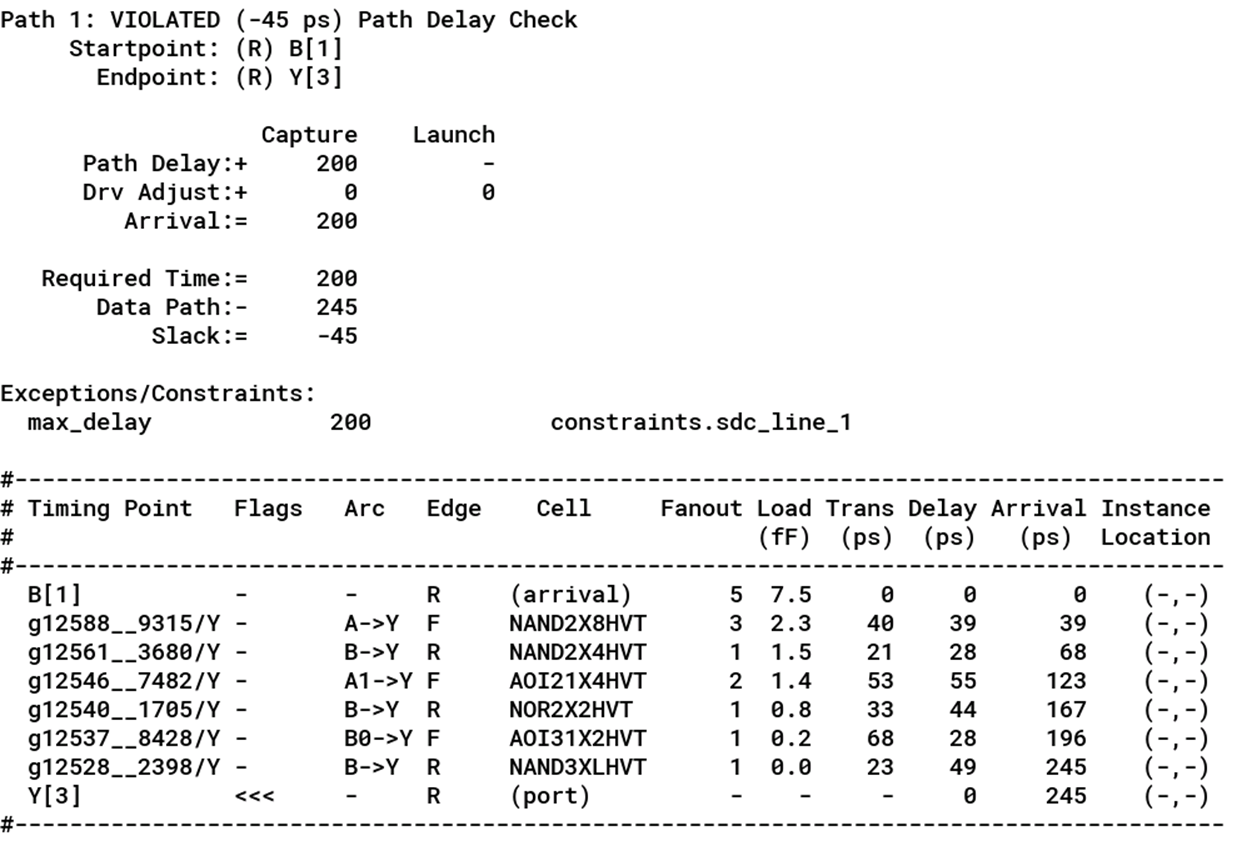
\includegraphics[width=0.8\linewidth]{figure/exp2_0.2ns_report.png}
    \caption{Chi tiết báo cáo thời gian tại mốc Max Delay = 0.2 ns}
    \label{fig:exp2_02ns_report}
\end{figure}

\begin{itemize}
    \item \textbf{Đường đi tín hiệu:} \texttt{B[1]} $\rightarrow$ NAND2X8HVT $\rightarrow$ NAND2X4HVT $\rightarrow$ AOI21X4HVT $\rightarrow$ NOR2X2HVT $\rightarrow$ AOI31X2HVT $\rightarrow$ NAND3XLHVT $\rightarrow$ \texttt{Y[3]}.
    \item \textbf{Thời gian dữ liệu truyền:} 245 ps.
    \item \textbf{Thời gian yêu cầu:} 200 ps.
    \item \textbf{Thời gian dư:} 200 ps - 245 ps = -45 ps (Vi phạm - VIOLATED).
    \item \textbf{Kết luận:} Vi phạm Timing.
\end{itemize}

\begin{figure}[H]
    \centering
    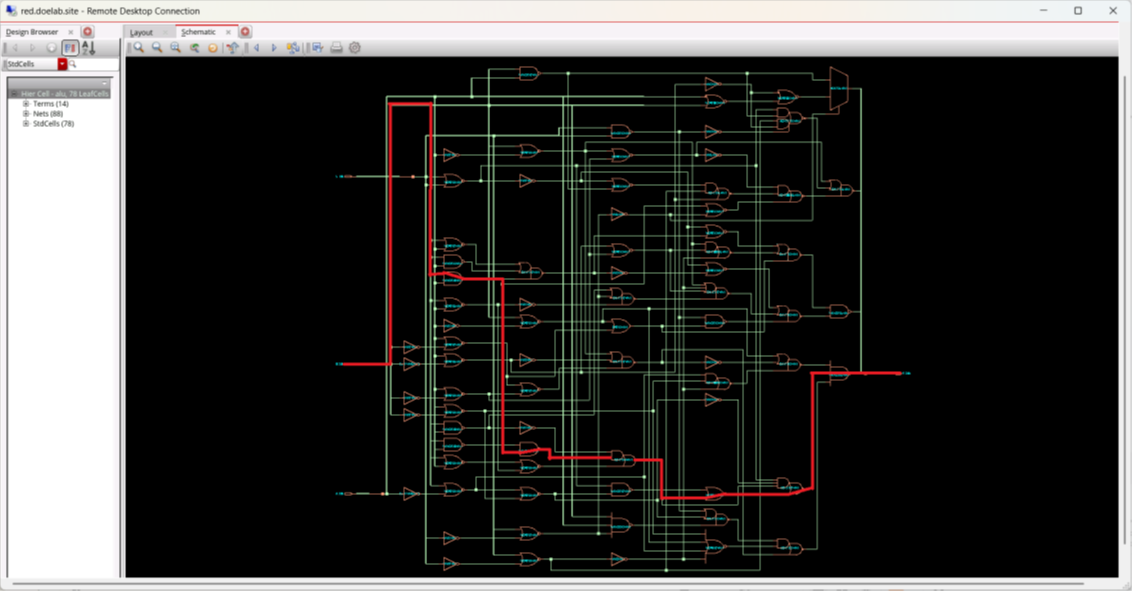
\includegraphics[width=\linewidth]{figure/exp2_0.2ns_schematic.png}
    \caption{Sơ đồ mạch hiển thị đường truyền tới hạn tại Max Delay = 0.2 ns}
    \label{fig:exp2_02ns_schematic}
\end{figure}

% ---------- Max Delay = 0.1 ns ----------
\subsubsection{Max Delay = 0.1 ns}

\begin{figure}[H]
    \centering
    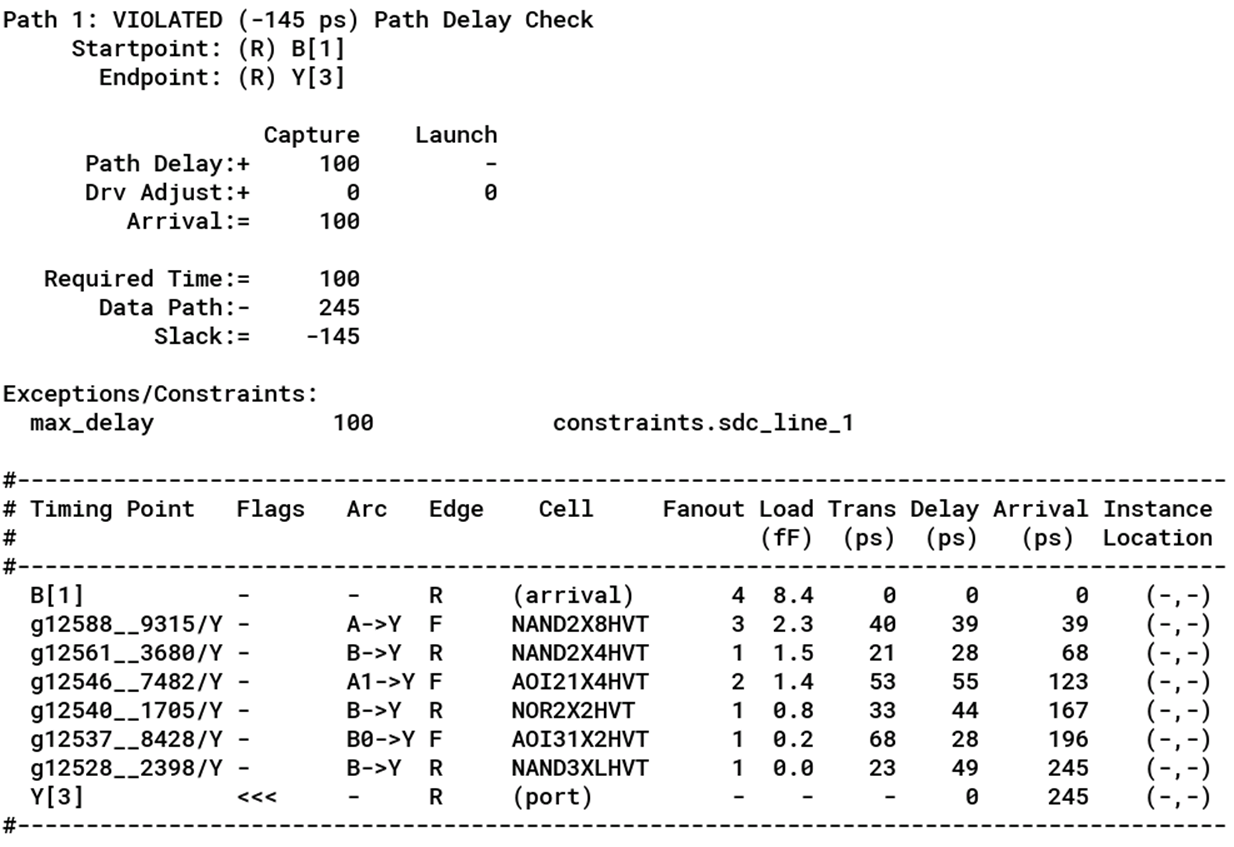
\includegraphics[width=0.8\linewidth]{figure/exp2_0.1ns_report.png}
    \caption{Chi tiết báo cáo thời gian tại mốc Max Delay = 0.1 ns}
    \label{fig:exp2_01ns_report}
\end{figure}

\begin{itemize}
    \item \textbf{Đường đi tín hiệu:} \texttt{B[1]} $\rightarrow$ NAND2X8HVT $\rightarrow$ NAND2X8HVT $\rightarrow$ AOI21X4HVT $\rightarrow$ NOR2X2HVT $\rightarrow$ AOI31X2HVT $\rightarrow$ NAND3XLHVT $\rightarrow$ \texttt{Y[3]}.
    \item \textbf{Thời gian dữ liệu truyền:} 245 ps.
    \item \textbf{Thời gian yêu cầu:} 100 ps.
    \item \textbf{Thời gian dư:} 100 ps - 245 ps = -145 ps (Vi phạm - VIOLATED).
    \item \textbf{Kết luận:} Vi phạm Timing.
\end{itemize}

\begin{figure}[H]
    \centering
    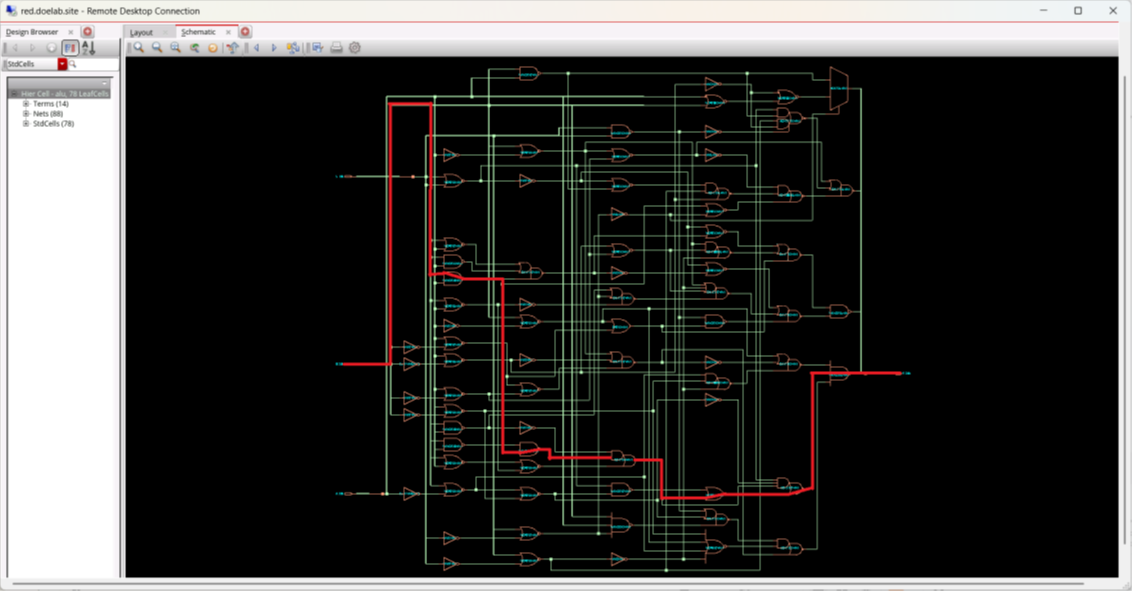
\includegraphics[width=\linewidth]{figure/exp2_0.1ns_schematic.png}
    \caption{Sơ đồ mạch hiển thị đường truyền tới hạn tại Max Delay = 0.1 ns}
    \label{fig:exp2_01ns_schematic}
\end{figure}

% ---------- Phần 2.2 ----------
\subsection{Nhận xét hành vi tối ưu hóa của công cụ Genus}

Kết quả của Experiment 2 cho thấy ràng buộc timing đóng vai trò quyết định trong quá trình tổng hợp và tối ưu mạch ALU:

\begin{itemize}
    \item Ở các mức max delay lớn (10 ns và 1 ns), mạch đáp ứng yêu cầu timing với slack dương lớn, chứng tỏ độ trễ của đường truyền xấu nhất nhỏ hơn nhiều so với giới hạn cho phép. Trong các trường hợp này, công cụ Genus không cần thực hiện tối ưu timing mạnh, do đó mạch sau synthesis có cấu trúc đơn giản và mức độ sử dụng các cell có tốc độ cao là không đáng kể.
    \item Khi ràng buộc timing được siết chặt xuống 0.5 ns, mạch vẫn đáp ứng yêu cầu timing nhưng slack giảm đáng kể, cho thấy đường truyền xấu nhất đã tiệm cận giới hạn max delay. Điều này phản ánh việc Genus đã phải thực hiện các chiến lược tối ưu timing như lựa chọn các cell có drive strength lớn hơn và sắp xếp lại cấu trúc logic nhằm giảm độ trễ đường truyền. Tuy nhiên, khả năng tối ưu vẫn còn bị giới hạn bởi đặc tính công nghệ của thư viện cell được sử dụng.
    \item Ở các mức max delay nhỏ hơn (0.2 ns và 0.1 ns), kết quả phân tích STA cho thấy mạch xuất hiện vi phạm timing với slack âm. Điều này cho thấy yêu cầu timing trong các trường hợp này vượt quá khả năng đáp ứng vật lý của mạch tổ hợp ALU khi sử dụng công nghệ 45 nm và thư viện \texttt{slow\_vdd1v2\_basicCells\_hvt.lib}. Mặc dù công cụ Genus đã sử dụng các cell có tốc độ cao hơn và gia tăng mức độ tối ưu, độ trễ tối thiểu của đường truyền logic vẫn không thể giảm xuống thấp hơn giới hạn yêu cầu.
\end{itemize}

\textbf{Tổng kết:} Từ các kết quả trên có thể kết luận rằng việc giảm max delay giúp cải thiện tốc độ mạch nhưng đồng thời làm tăng độ phức tạp của mạch và nguy cơ vi phạm timing. Do đó, trong thực tế thiết kế, ràng buộc timing cần được lựa chọn phù hợp với công nghệ chế tạo và thư viện cell nhằm đạt được sự cân bằng hợp lý giữa hiệu năng và khả năng thực hiện của mạch.

\newpage
% ================= EXPERIMENT 3 =================
\section{Experiment 3: Timing analysis for sequential circuits after synthesis}
\textit{Khảo sát mạch tuần tự sử dụng thư viện \texttt{slow\_vdd1v2\_basicCells\_hvt.lib}.}

\subsection{Code RTL của mạch tuần tự ALU}
\textit{Ghi chú: Chèn đoạn code HDL chứa block \texttt{always\_ff @ (posedge clk)} mô tả mạch ALU tuần tự vào đây.}

\subsection{Ràng buộc thời gian (SDC) cho mạch tuần tự}
Đối với mạch tuần tự ALU (hoạt động đồng bộ theo xung nhịp), file constraints được bổ sung thêm việc khởi tạo clock và thiết lập độ trễ an toàn cho ngõ vào/ngõ ra. Dưới đây là cấu hình mặc định được sử dụng:

\textbf{File constraints.sdc (Mặc định):}
\begin{verbatim}
create_clock -name clk -period 1.0 [get_ports clk]
set_input_delay 0.2 -clock [get_clocks *] [all_inputs]
set_output_delay 0.3 -clock [get_clocks *] [all_outputs]
set_max_delay 0.5 -from [all_inputs] -to [all_outputs]
set timing_report_unconstrained true
\end{verbatim}
Ý nghĩa: 
\begin{itemize}
    \item Khởi tạo xung nhịp \texttt{clk} với chu kỳ 1.0 ns.
    \item Tín hiệu ngõ vào sẽ đến chậm 0.2 ns sau sườn clock.
    \item Dữ liệu ngõ ra phải ổn định 0.3 ns trước sườn clock tiếp theo.
    \item Độ trễ lớn nhất qua các cổng logic tổ hợp bên trong mạch không vượt quá 0.5 ns.
\end{itemize}


\subsection{Phân tích Timing với ràng buộc SDC mặc định}
\textit{Sử dụng SDC mặc định: \texttt{period=1.0}, \texttt{max\_delay=0.5}, \texttt{input\_delay=0.2}, \texttt{output\_delay=0.3}}

\textbf{A. Phân tích đường truyền tới hạn} \\
Dựa trên ràng buộc timing với chu kỳ xung nhịp (clock) = 1.0 ns và trễ ngõ vào (input\_delay) = 0.2 ns, đường truyền có độ trễ lớn nhất của mạch tuần tự ALU được xác định với các thông số sau: %[cite: 3]

\begin{figure}[H]
    \centering
    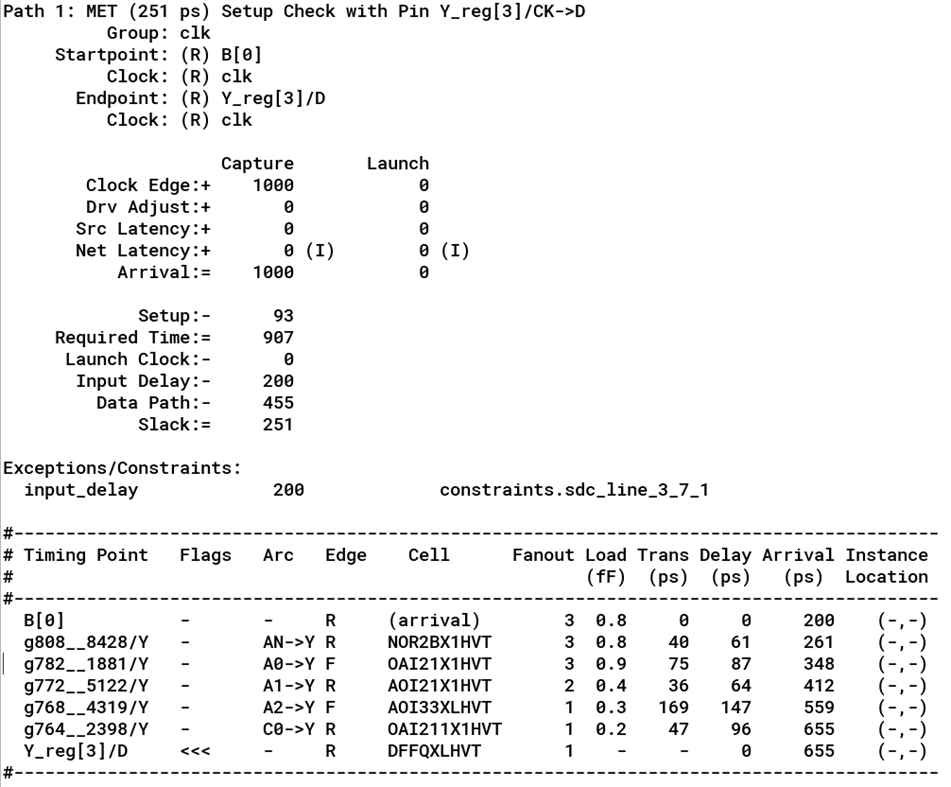
\includegraphics[width=0.8\linewidth]{figure/exp3_default_path1_report.png}
    \caption{Chi tiết báo cáo Setup Check của đường truyền tới hạn mạch tuần tự} %[cite: 3]
    \label{fig:exp3_def_report}
\end{figure}

Đường truyền bắt đầu từ ngõ vào \texttt{B[0]} và kết thúc tại chân D của flip-flop \texttt{Y\_reg[3]}. %[cite: 3]
\begin{itemize}
    \item \textbf{Đường đi tín hiệu:} B[0] $\rightarrow$ NOR2BX1HVT $\rightarrow$ OAI21X1HVT $\rightarrow$ AOI21X1HVT $\rightarrow$ AOI33XLHVT $\rightarrow$ OAI211X1HVT $\rightarrow$ Y\_reg[3]/D (DFFQXLHVT). 
    \item \textbf{Tổng thời gian tín hiệu đến đích:} 655 ps. Con số này bao gồm 200 ps độ trễ đầu vào + 455 ps độ trễ truyền qua các cổng logic. 
    \item \textbf{Thời gian yêu cầu:} 907 ps. Cần đảm bảo dữ liệu ổn định trước sườn xung nhịp, tính bằng chu kỳ clock (1000 ps) trừ đi thời gian setup của flip-flop (93 ps).
    \item \textbf{Thời gian dư:} Required Time - Arrival Time = 907 ps - 655 ps = 251 ps (Đạt - MET).
    \item \textbf{Kết luận:} Vì Slack mang giá trị dương ($>0$), đường truyền tới hạn thỏa mãn các ràng buộc timing đã đặt ra và không bị vi phạm.
\end{itemize}

\begin{figure}[H]
    \centering
    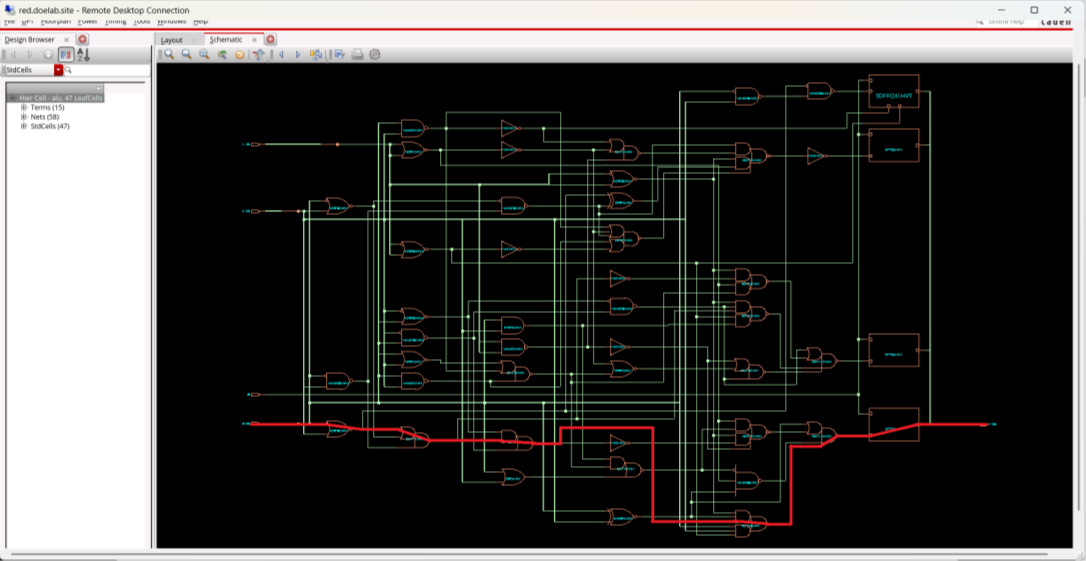
\includegraphics[width=\linewidth]{figure/exp3_default_path1_schematic.png}
    \caption{Sơ đồ mạch hiển thị đường truyền tới hạn với SDC mặc định} %[cite: 3]
    \label{fig:exp3_def_schematic}
\end{figure}

\textbf{B. Phân tích 10 đường truyền trễ nhất (10 Worst Paths Timing Analysis)}
\begin{table}[H]
    \centering
    \resizebox{\textwidth}{!}{
    \begin{tabular}{|c|l|p{9cm}|c|c|c|c|c|}
        \hline
        \textbf{STT} & \textbf{Startpoint $\rightarrow$ Endpoint} & \textbf{Đường đi tín hiệu (Traversal)} & \textbf{Data Path} & \textbf{In Delay} & \textbf{Req Time} & \textbf{Slack} & \textbf{Trạng thái} \\
        \hline
        1 & B[0] $\rightarrow$ Y\_reg[3]/D & B[0] $\rightarrow$ NOR2BX1HVT $\rightarrow$ OAI21X1HVT $\rightarrow$ AOI21X1HVT $\rightarrow$ AOI33XLHVT $\rightarrow$ OAI211X1HVT $\rightarrow$ DFFQXLHVT & 455 & 200 & 907 & 251 & MET \\ \hline %[cite: 3]
        2 & B[1] $\rightarrow$ Y\_reg[3]/D & B[1] $\rightarrow$ NOR2BX1HVT $\rightarrow$ OAI21X1HVT $\rightarrow$ AOI21X1HVT $\rightarrow$ AOI33XLHVT $\rightarrow$ OAI211X1HVT $\rightarrow$ DFFQXLHVT & 436 & 200 & 907 & 270 & MET \\ \hline %[cite: 3]
        3 & A[0] $\rightarrow$ Y\_reg[3]/D & A[0] $\rightarrow$ NOR2BX1HVT $\rightarrow$ OAI21X1HVT $\rightarrow$ AOI21X1HVT $\rightarrow$ AOI33XLHVT $\rightarrow$ OAI211X1HVT $\rightarrow$ DFFQXLHVT & 422 & 200 & 907 & 285 & MET \\ \hline %[cite: 3]
        4 & B[1] $\rightarrow$ Y\_reg[3]/D & B[1] $\rightarrow$ NAND2BX1HVT $\rightarrow$ OAI21X1HVT $\rightarrow$ AOI21X1HVT $\rightarrow$ AOI33XLHVT $\rightarrow$ OAI211X1HVT $\rightarrow$ DFFQXLHVT & 422 & 200 & 907 & 285 & MET \\ \hline %[cite: 3]
        5 & A[1] $\rightarrow$ Y\_reg[3]/D & A[1] $\rightarrow$ NOR2BX1HVT $\rightarrow$ OAI21X1HVT $\rightarrow$ AOI21X1HVT $\rightarrow$ AOI33XLHVT $\rightarrow$ OAI211X1HVT $\rightarrow$ DFFQXLHVT & 403 & 200 & 907 & 304 & MET \\ \hline %[cite: 3]
        6 & B[0] $\rightarrow$ Y\_reg[3]/D & B[0] $\rightarrow$ NOR2BX1HVT $\rightarrow$ OAI21X1HVT $\rightarrow$ AOI21X1HVT $\rightarrow$ INVXLHVT $\rightarrow$ AOI221X1HVT $\rightarrow$ OAI211X1HVT $\rightarrow$ DFFQXLHVT & 421 & 200 & 936 & 315 & MET \\ \hline %[cite: 3]
        7 & A[1] $\rightarrow$ Y\_reg[3]/D & A[1] $\rightarrow$ NAND2BX1HVT $\rightarrow$ OAI21X1HVT $\rightarrow$ AOI21X1HVT $\rightarrow$ AOI33XLHVT $\rightarrow$ OAI211X1HVT $\rightarrow$ DFFQXLHVT & 391 & 200 & 907 & 316 & MET \\ \hline %[cite: 3]
        8 & B[0] $\rightarrow$ Y\_reg[3]/D & B[0] $\rightarrow$ NAND2X1HVT $\rightarrow$ OAI21X1HVT $\rightarrow$ AOI21X1HVT $\rightarrow$ NAND3BXLHVT $\rightarrow$ OAI211X1HVT $\rightarrow$ DFFQXLHVT & 384 & 200 & 907 & 322 & MET \\ \hline %[cite: 3]
        9 & B[3] $\rightarrow$ Y\_reg[3]/D & B[3] $\rightarrow$ XNOR2X1HVT $\rightarrow$ AOI33XLHVT $\rightarrow$ OAI211X1HVT $\rightarrow$ DFFQXLHVT & 383 & 200 & 907 & 323 & MET \\ \hline %[cite: 3]
        10 & B[0] $\rightarrow$ Y\_reg[3]/D & B[0] $\rightarrow$ NAND2X1HVT $\rightarrow$ OAI21X1HVT $\rightarrow$ AOI21X1HVT $\rightarrow$ AOI221X1HVT $\rightarrow$ OAI211X1HVT $\rightarrow$ DFFQXLHVT & 408 & 200 & 936 & 328 & MET \\ \hline %[cite: 3]
    \end{tabular}
    }
    \caption{Bảng tổng hợp 10 đường truyền trễ nhất (Dữ liệu tính bằng ps)}
\end{table}

\subsection{Khảo sát Timing với các kịch bản Constraint (Scenarios)}

% ---------- Scenario 1 ----------
\subsubsection{Scenario 1: \texttt{period=1ns, max\_delay=0.2ns, input=0.2ns, output=0.3ns}}

\begin{figure}[H]
    \centering
    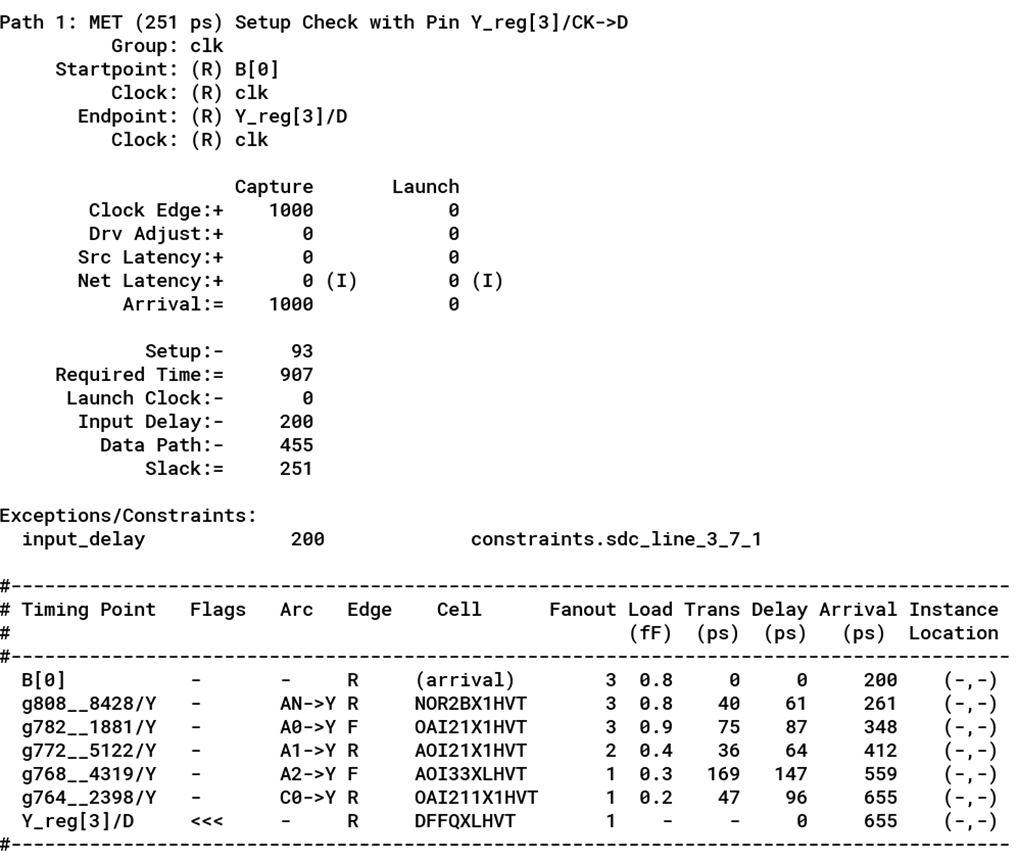
\includegraphics[width=0.8\linewidth]{figure/exp3_scen1_report.png}
    \caption{Chi tiết báo cáo thời gian tại Scenario 1}
    \label{fig:exp3_s1_report}
\end{figure}

\begin{itemize}
    \item \textbf{Đường đi tín hiệu:} B[0] $\rightarrow$ NOR2BX1HVT $\rightarrow$ OAI21X1HVT $\rightarrow$ AOI21X1HVT $\rightarrow$ AOI33XLHVT $\rightarrow$ OAI211X1HVT $\rightarrow$ Y\_reg[3]/D. 
    \item \textbf{Thời gian dư:} 251 ps (Đạt - MET). 
    \item \textbf{Kết luận:} Đường truyền này đáp ứng tốt các yêu cầu về thời gian. Đặc tả này trùng khớp với trường hợp cấu hình mặc định ở mục 3.2. 
\end{itemize}

\begin{figure}[H]
    \centering
    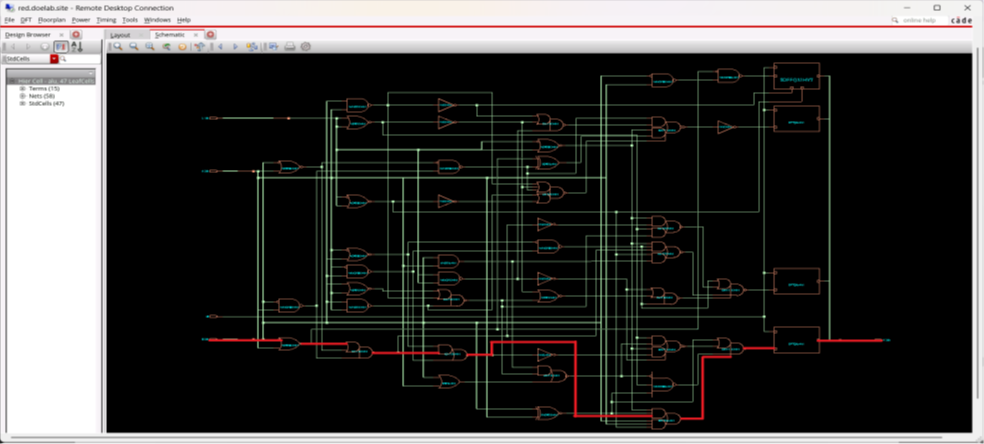
\includegraphics[width=\linewidth]{figure/exp3_scen1_schematic.png}
    \caption{Sơ đồ mạch hiển thị đường truyền tới hạn tại Scenario 1}
    \label{fig:exp3_s1_schematic}
\end{figure}

% ---------- Scenario 2 ----------
\subsubsection{Scenario 2: \texttt{period=1ns, max\_delay=0.2ns, input=0.1ns, output=0.3ns}}

\begin{figure}[H]
    \centering
    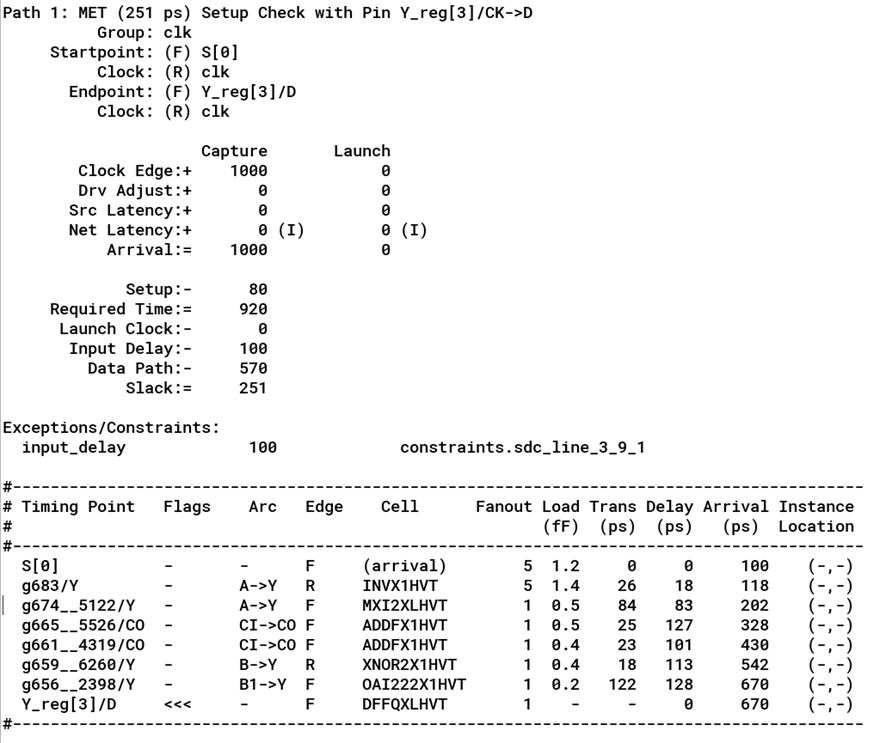
\includegraphics[width=0.8\linewidth]{figure/exp3_scen2_report.png}
    \caption{Chi tiết báo cáo thời gian tại Scenario 2}
    \label{fig:exp3_s2_report}
\end{figure}

\begin{itemize}
    \item \textbf{Đường đi tín hiệu:} S[0] $\rightarrow$ INVX1HVT $\rightarrow$ MXI2XLHVT $\rightarrow$ ADDFX1HVT $\rightarrow$ ADDFX1HVT $\rightarrow$ XNOR2X1HVT $\rightarrow$ OAI222X1HVT $\rightarrow$ Y\_reg[3]/D. 
    \item \textbf{Thông số trễ:} \texttt{Arrival Time} = 100 ps (input delay) + 570 ps (data path) = 670 ps. \texttt{Required Time} = 1000 ps - 80 ps = 920 ps.
    \item \textbf{Thời gian dư:} 920 ps - 670 ps = 251 ps (Đạt - MET).
    \item \textbf{Kết luận:} Không vi phạm timing. Cấu trúc mạch tối ưu khác đi do ràng buộc ngõ vào được thu hẹp (input\_delay giảm). 
\end{itemize}

\begin{figure}[H]
    \centering
    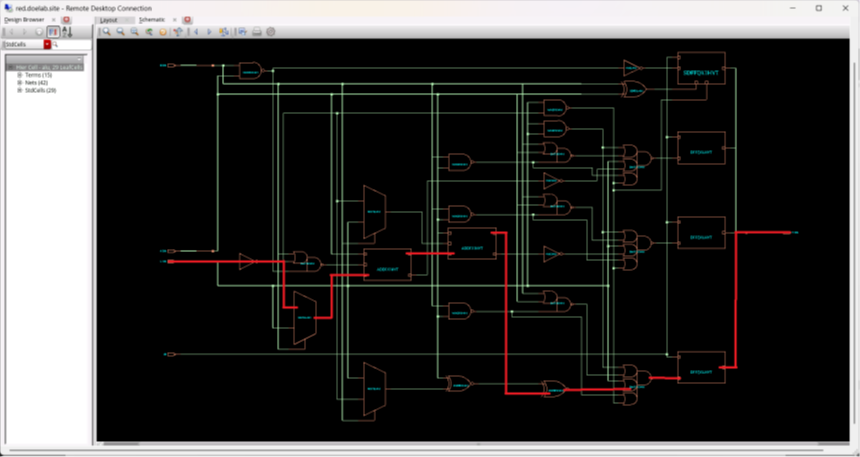
\includegraphics[width=\linewidth]{figure/exp3_scen2_schematic.png}
    \caption{Sơ đồ mạch hiển thị đường truyền tới hạn tại Scenario 2}
    \label{fig:exp3_s2_schematic}
\end{figure}

% ---------- Scenario 3 ----------
\subsubsection{Scenario 3: \texttt{period=0.8ns, max\_delay=0.2ns, input=0.3ns, output=0.3ns}}

\begin{figure}[H]
    \centering
    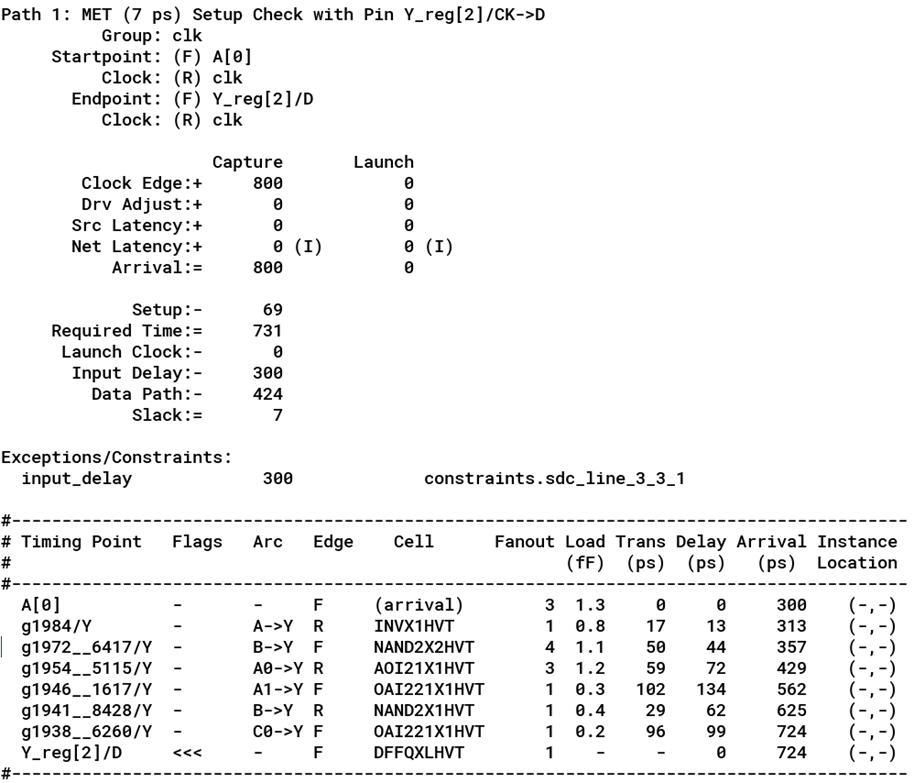
\includegraphics[width=0.8\linewidth]{figure/exp3_scen3_report.png}
    \caption{Chi tiết báo cáo thời gian tại Scenario 3}
    \label{fig:exp3_s3_report}
\end{figure}

\begin{itemize}
    \item \textbf{Đường đi tín hiệu:} A[0] $\rightarrow$ INVX1HVT $\rightarrow$ NAND2X2HVT $\rightarrow$ AOI21X1HVT $\rightarrow$ OAI221X1HVT $\rightarrow$ NAND2X1HVT $\rightarrow$ OAI221X1HVT $\rightarrow$ Y\_reg[2]/D. %[cite: 3]
    \item \textbf{Thông số trễ:} \texttt{Arrival Time} = 300 ps + 424 ps = 724 ps. \texttt{Required Time} = 800 ps - 69 ps = 731 ps. %[cite: 3]
    \item \textbf{Thời gian dư:} 731 ps - 724 ps = 7 ps (Đạt - MET). %[cite: 3]
    \item \textbf{Kết luận:} Khi rút ngắn chu kỳ clock xuống 0.8 ns và tăng input delay lên 0.3 ns, đường truyền đã tiệm cận rất sát giới hạn vi phạm (chỉ dư 7 ps). %[cite: 3]
\end{itemize}

\begin{figure}[H]
    \centering
    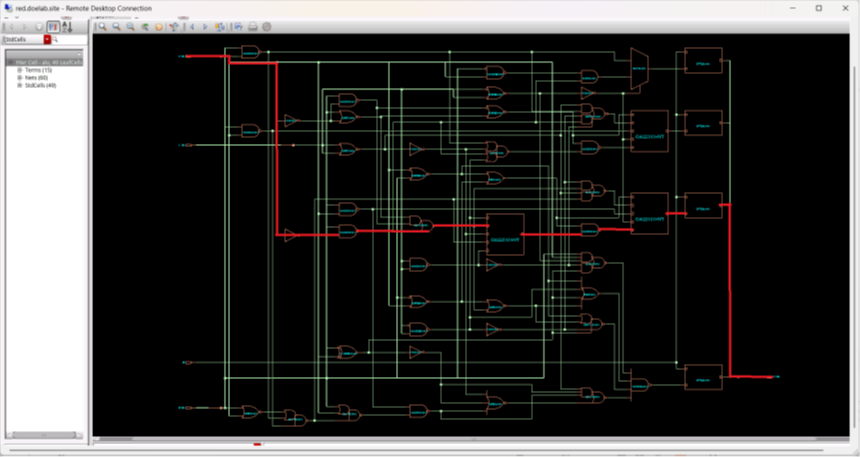
\includegraphics[width=\linewidth]{figure/exp3_scen3_schematic.png}
    \caption{Sơ đồ mạch hiển thị đường truyền tới hạn tại Scenario 3}
    \label{fig:exp3_s3_schematic}
\end{figure}

% ---------- Scenario 4 ----------
\subsubsection{Scenario 4: \texttt{period=0.6ns, max\_delay=0.2ns, input=0.2ns, output=0.2ns}}

\begin{figure}[H]
    \centering
    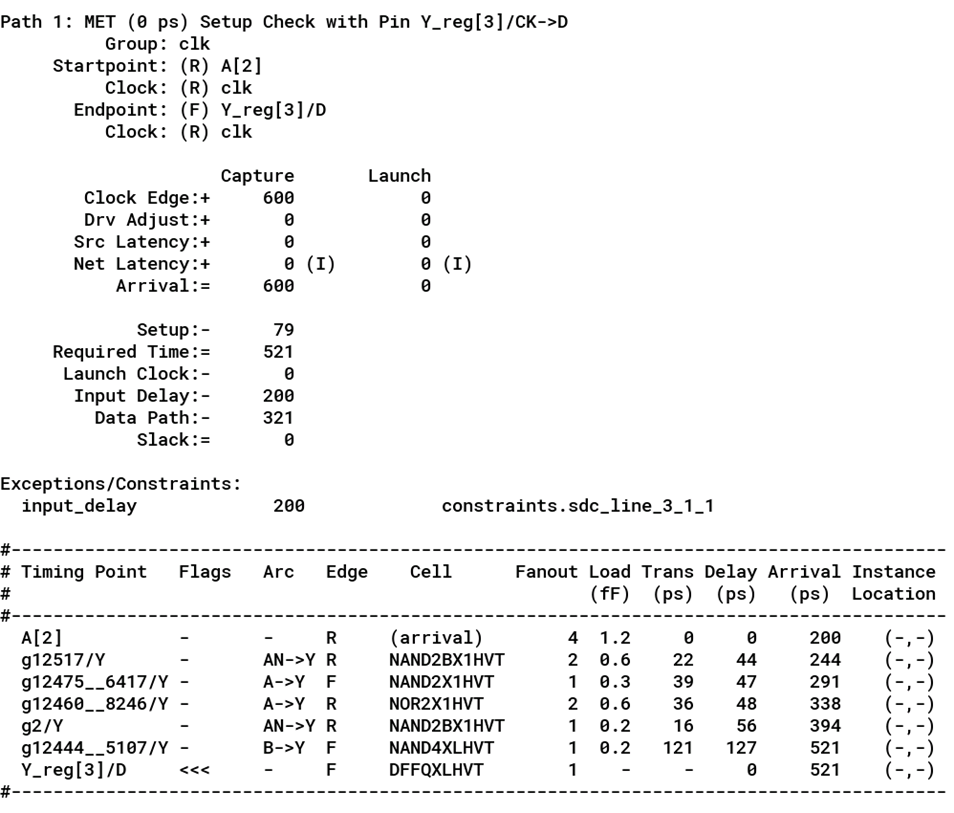
\includegraphics[width=0.8\linewidth]{figure/exp3_scen4_report.png}
    \caption{Chi tiết báo cáo thời gian tại Scenario 4}
    \label{fig:exp3_s4_report}
\end{figure}

\begin{itemize}
    \item \textbf{Đường đi tín hiệu:} A[2] $\rightarrow$ NAND2BX1HVT $\rightarrow$ NAND2X1HVT $\rightarrow$ NOR2X1HVT $\rightarrow$ NAND2BX1HVT $\rightarrow$ NAND4XLHVT $\rightarrow$ Y\_reg[3]/D.
    \item \textbf{Thông số trễ:} \texttt{Arrival Time} = 200 ps + 321 ps = 521 ps. \texttt{Required Time} = 600 ps - 79 ps = 521 ps.
    \item \textbf{Thời gian dư:} 521 ps - 521 ps = 0 ps (Đạt - MET).
    \item \textbf{Kết luận:} Mạch đạt giới hạn tối đa, Slack vừa tròn 0 ps, không vi phạm timing. %
\end{itemize}

\begin{figure}[H]
    \centering
    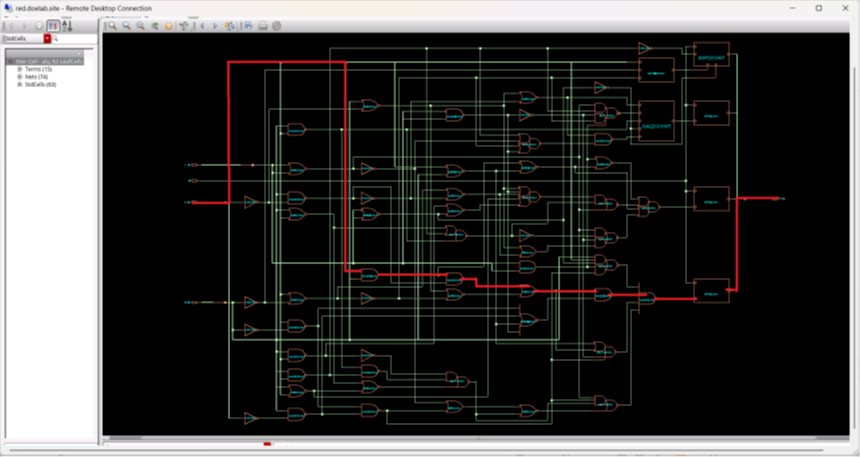
\includegraphics[width=\linewidth]{figure/exp3_scen4_schematic.png}
    \caption{Sơ đồ mạch hiển thị đường truyền tới hạn tại Scenario 4}
    \label{fig:exp3_s4_schematic}
\end{figure}

% ---------- Scenario 5 ----------
\subsubsection{Scenario 5: \texttt{period=0.5ns, max\_delay=0.2ns, input=0.1ns, output=0.2ns}}

\begin{figure}[H]
    \centering
    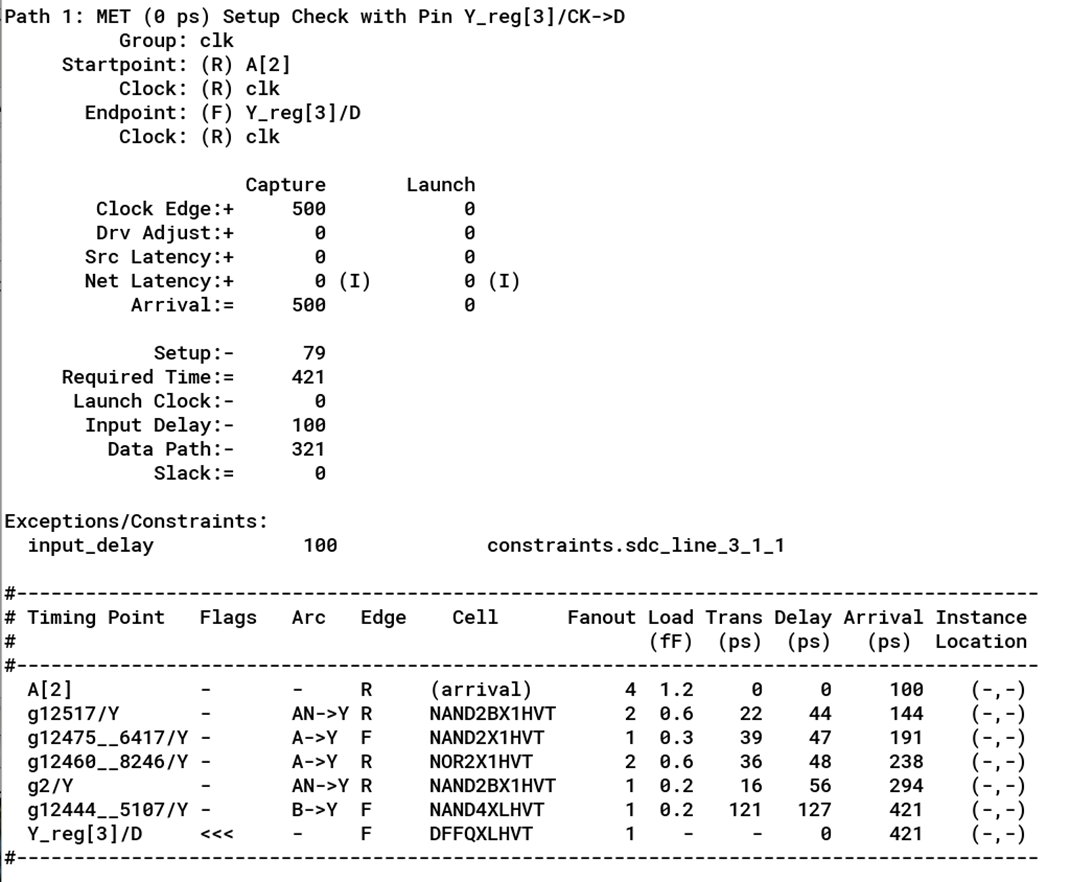
\includegraphics[width=0.8\linewidth]{figure/exp3_scen5_report.png}
    \caption{Chi tiết báo cáo thời gian tại Scenario 5}
    \label{fig:exp3_s5_report}
\end{figure}

\begin{itemize}
    \item \textbf{Đường đi tín hiệu:} A[2] $\rightarrow$ NAND2BX1HVT $\rightarrow$ NAND2X1HVT $\rightarrow$ NOR2X1HVT $\rightarrow$ NAND2BX1HVT $\rightarrow$ NAND4XLHVT $\rightarrow$ Y\_reg[3]/D. 
    \item \textbf{Thông số trễ:} \texttt{Arrival Time} = 100 ps + 321 ps = 421 ps. \texttt{Required Time} = 500 ps - 79 ps = 421 ps.
    \item \textbf{Thời gian dư (Slack):} 421 ps - 421 ps = 0 ps (Đạt - MET). %[cite: 3]
    \item \textbf{Kết luận:} Ở điều kiện khắc nghiệt nhất (chu kỳ xung nhịp ép xuống 0.5 ns), hệ thống vẫn vừa vặn đáp ứng (MET) với Slack = 0 ps. Công cụ Genus đã tối ưu logic triệt để để giảm độ trễ qua cổng xuống mức thấp nhất có thể là 321 ps. 
\end{itemize}

\begin{figure}[H]
    \centering
    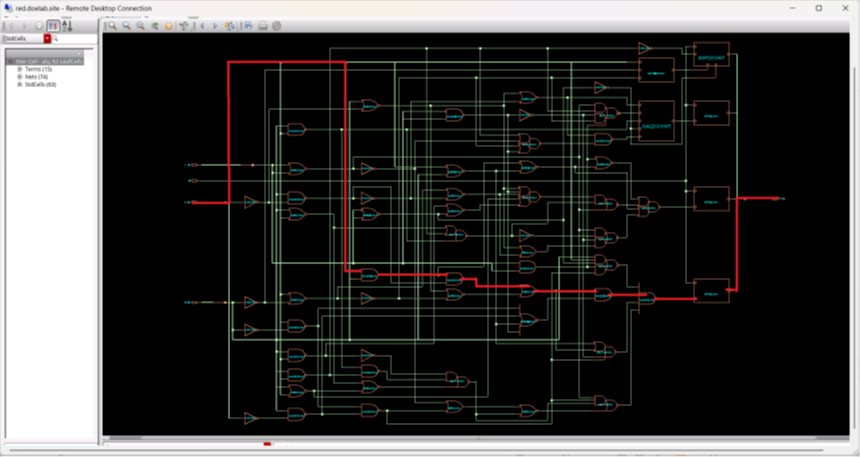
\includegraphics[width=\linewidth]{figure/exp3_scen5_schematic.png}
    \caption{Sơ đồ mạch hiển thị đường truyền tới hạn tại Scenario 5}
    \label{fig:exp3_s5_schematic}
\end{figure}

% ---------- Tổng kết ----------
\subsection{Nhận xét tổng kết Experiment 3}
Qua 5 kịch bản khảo sát thời gian trên mạch tuần tự, ta thấy rõ sự tương quan giữa các thông số SDC: \texttt{period} (chu kỳ xung nhịp), \texttt{input\_delay} (trễ ngõ vào) và khả năng đáp ứng timing của mạch:
\begin{itemize}
    \item \textbf{Chu kỳ xung nhịp:} Việc giảm \texttt{period} (từ 1.0 ns xuống 0.5 ns) là yếu tố trực tiếp nhất làm thu hẹp \texttt{Required Time}. Khi chu kỳ bị ép ngắn lại, quỹ thời gian dành cho tín hiệu lan truyền qua các cổng logic tổ hợp (giữa các flip-flop) bị giảm mạnh. Ở các Kịch bản 4 và 5, mạch bị ép tới giới hạn cực đại (Slack = 0).
    \item \textbf{Trễ ngõ vào:} Thông số này ăn trực tiếp vào quỹ thời gian tín hiệu bắt đầu (Arrival Time). Khi tăng \texttt{input\_delay}, \texttt{Arrival Time} tăng lên, khiến nguy cơ vi phạm Setup time lớn hơn.
    \item \textbf{Hành vi tối ưu của công cụ tổng hợp:} Để mạch luôn đạt trạng thái MET, khi các ràng buộc ngày càng siết chặt, công cụ Genus đã chủ động chọn lại các phần tử thư viện có drive strength mạnh hơn và tối giản hóa độ sâu của tầng logic. Bằng chứng là Data path (thời gian lan truyền thực tế qua cổng) đã được ép từ 455 ps (Kịch bản 1) xuống chỉ còn 321 ps (Kịch bản 4, 5) để vượt qua bài kiểm tra Setup Check khắt khe nhất.
\end{itemize}
\end{document}